%-----------------------------------------------------------------------
% Beginning of chapter.tex
%-----------------------------------------------------------------------
%
%  This is a sample file for use with AMS-LaTeX.  It provides an example
%  of how to set up a file for a book to be typeset with AMS-LaTeX.
%
%  This is the driver file.  Separate chapters should be included at
%  the end of this file.
%
%  ***** DO NOT USE THIS FILE AS A STARTER FOR YOUR BOOK. *****
%  Follow the guidelines in the file chapter.template.
%
%%%%%%%%%%%%%%%%%%%%%%%%%%%%%%%%%%%%%%%%%%%%%%%%%%%%%%%%%%%%%%%%%%%%%%%%

\documentclass[12pt,a4paper]{memoir}
\chapterstyle{demo}
\epigraphfontsize{\small\itshape}
\setlength\epigraphwidth{8cm}
\setlength\epigraphrule{0pt}
\epigraphfontsize{\small\itshape}

\evensidemargin=0in
\oddsidemargin=0in
\textwidth=6.3in
\topmargin=-0.33in
\headheight=0.25in
\textheight=9in

% Include macros here
%=================================================
% Packages
%=================================================

\usepackage{fixltx2e}
\usepackage[usenames,dvipsnames]{xcolor}
\usepackage{fancyhdr}
\usepackage{amsmath,amsfonts,amsbsy,amsgen,amscd,mathrsfs,amssymb}
%\usepackage{amsthm}
\usepackage{subfig}
\usepackage{url}
\usepackage{tikz}
\usepackage{enumitem}
\usepackage{listings}
\lstset{language=Matlab}

\newtheorem{theorem}{Theorem}[section]
\newtheorem{lemma}[theorem]{Lemma}
\newtheorem{corollary}[theorem]{Corollary}
\newtheorem{proposition}[theorem]{Proposition}
\newtheorem{remark}[theorem]{Remark}
\newtheorem{definition}[theorem]{Definition}
\newtheorem{example}[theorem]{Example}
%\newtheorem{remark}[theorem]{Remark}

\numberwithin{equation}{section}

\definecolor{dark-gray}{gray}{0.3}
\usepackage[colorlinks=true]{hyperref}
\hypersetup{urlcolor=Blue}
\hypersetup{citecolor=Black}
\hypersetup{linkcolor=dark-gray}

\usepackage{setspace}
\usepackage{graphicx}
\usepackage{booktabs,longtable,tabu} % Nice tables
\setlength{\tabulinesep}{1pt}
\usepackage{multirow} % More control over tables

% Fonts
%\usepackage{times}
\usepackage{fourier}
\usepackage{bm} % boldmath must be called after the package

%\usepackage{hyperref}
%\usepackage[notcite]{showkeys}
%\usepackage{bbm}  % Loads too many fonts :(
%\usepackage{euscript}
%\usepackage{latexsym}
%\usepackage{color}
%\usepackage[margin=1.25in]{geometry}
%\usepackage{thmtools}
%\usepackage{url}
%\usepackage{citesort}
%\usepackage{supertabular}
%\usepackage[font=small,margin=10pt,labelfont={bf},labelsep={space}]{caption}
%\usepackage{pstricks}

%=================================================
% Paths
%=================================================

\graphicspath{{figures/}}

%=================================================
% Formatting
%=================================================

\sloppy % Helps with margin justification

%%% Further font changes
\newcommand{\lang}{\textit}
\newcommand{\titl}{\textsl}
\newcommand{\term}{\emph}

%%% Equation numbering
\numberwithin{equation}{section} 

%%% Typesetting
\providecommand{\mathbold}[1]{\bm{#1}}  % Must be after 'fourier'
                                % package loads
%%% Annotations
\newcommand{\notate}[1]{\textcolor{red}{\textbf{[#1]}}}

%=================================================
% Theorem environment
%=================================================


%=================================================
% Symbols
%=================================================

%%% Old symbols with new names
\newcommand{\oldphi}{\phi}
\renewcommand{\phi}{\varphi}

\newcommand{\eps}{\varepsilon}
\newcommand{\e}{\varepsilon}

\newcommand{\oldmid}{\mid}
\renewcommand{\mid}{\mathrel{\mathop{:}}} 

%%% New symbols
\newcommand{\defby}{\overset{\mathrm{\scriptscriptstyle{def}}}{=}}
\newcommand{\half}{\tfrac{1}{2}}
\newcommand{\third}{\tfrac{1}{3}}

\newcommand{\sumnl}{\sum\nolimits}

\newcommand{\defeq}{\ensuremath{\mathrel{\mathop{:}}=}} % Definition-equals
\newcommand{\eqdef}{\ensuremath{=\mathrel{\mathop{:}}}} % Equals-definition

%%% Constants
\newcommand{\cnst}[1]{\mathrm{#1}} 
\newcommand{\econst}{\mathrm{e}}
\newcommand{\iunit}{\mathrm{i}}

\newcommand{\onevct}{\mathbf{e}} % All ones vector
\newcommand{\zerovct}{\vct{0}} % Zero vector

\newcommand{\Id}{\mathbf{I}}
\newcommand{\onemtx}{\bm{1}}
\newcommand{\zeromtx}{\bm{0}}

%%% Sets
\newcommand{\coll}[1]{\mathscr{#1}}
\newcommand{\sphere}[1]{\mathsf{S}^{#1}}
\newcommand{\ball}[1]{\mathsf{B}^{#1}}
\newcommand{\Grass}[2]{\mathsf{G}^{#1}_{#2}}
\providecommand{\mathbbm}{\mathbb} % In case we don't load bbm
\newcommand{\Rplus}{\mathbbm{R}_{+}}
\newcommand{\R}{\mathbbm{R}}
\newcommand{\C}{\mathbbm{C}}
\newcommand{\N}{\mathbbm{N}}

% Set operations
\newcommand{\polar}{\circ}
\newcommand{\closure}{\overline}

%%% Real and complex analysis
\newcommand{\abs}[1]{\left\vert {#1} \right\vert}
\newcommand{\abssq}[1]{{\abs{#1}}^2}

\newcommand{\sgn}[1]{\operatorname{sgn}{#1}}
\newcommand{\real}{\operatorname{Re}}
\newcommand{\imag}{\operatorname{Im}}
\newcommand{\pos}{\operatorname{Pos}}
\newcommand{\shrink}{\operatorname{Shrink}}

\newcommand{\diff}[1]{\mathrm{d}{#1}}
\newcommand{\idiff}[1]{\, \diff{#1}}


%\newcommand{\grad}{\nabla} % Conflicts w/SIAM styles?
\newcommand{\subdiff}{\partial}

\newcommand{\argmin}{\operatorname*{arg\; min}}
\newcommand{\argmax}{\operatorname*{arg\; max}}

%%% Probability & measure

\newcommand{\Prob}{\mathbbm{P}}
\newcommand{\Probe}[1]{\Prob\left({#1}\right)}
\newcommand{\Expect}{\operatorname{\mathbb{E}}}

\newcommand{\normal}{\textsc{Normal}}
\newcommand{\uniform}{\textsc{Uniform}}
\newcommand{\erf}{\operatorname{erf}}

\DeclareMathOperator{\rvol}{rvol}
\DeclareMathOperator{\Var}{Var}

%%% Vector and matrix operators
\newcommand{\vct}[1]{\mathbold{#1}}
\newcommand{\mtx}[1]{\mathbold{#1}}
\newcommand{\Eye}{\mathbf{I}}

\newcommand{\transp}{t}
\newcommand{\adj}{*}
\newcommand{\psinv}{\dagger}

\newcommand{\lspan}[1]{\operatorname{span}{#1}}

\newcommand{\range}{\operatorname{range}}
\newcommand{\colspan}{\operatorname{colspan}}

\newcommand{\rank}{\operatorname{rank}}
\newcommand{\nullity}{\operatorname{null}}

%\newcommand{\diag}{\operatorname{diag}}
\newcommand{\trace}{\operatorname{tr}}

%\newcommand{\supp}[1]{\operatorname{supp}(#1)}

\newcommand{\smax}{\sigma_{\max}}
\newcommand{\smin}{\sigma_{\min}}

\newcommand{\nnz}{\operatorname{nnz}}
\renewcommand{\vec}{\operatorname{vec}}

\newcommand{\Proj}{\ensuremath{\mtx{\Pi}}} % Projection operator

%%% Semidefinite orders
\newcommand{\psdle}{\preccurlyeq}
\newcommand{\psdge}{\succcurlyeq}

\newcommand{\psdlt}{\prec}
\newcommand{\psdgt}{\succ}

%%% Mensuration: inner products and norms

% TeX does not like either \newcommand or \renewcommand for these
% two macros.  There is probably a good reason not to use them via
% \def, but I don't know it.  
%\newcommand{\<}{\langle} 
%\newcommand{\>}{\rangle}
\newcommand{\ip}[2]{\left\langle {#1},\ {#2} \right\rangle}
\newcommand{\absip}[2]{\abs{\ip{#1}{#2}}}
\newcommand{\abssqip}[2]{\abssq{\ip{#1}{#2}}}
\newcommand{\tworealip}[2]{2 \, \real{\ip{#1}{#2}}}

\newcommand{\norm}[1]{\left\Vert {#1} \right\Vert}
\newcommand{\normsq}[1]{\norm{#1}^2}

\newcommand{\lone}[1]{\norm{#1}_{\ell_1}}
\newcommand{\smlone}[1]{\|#1\|_{\ell_1}}
\newcommand{\linf}[1]{\norm{#1}_{\ell_\infty}}
\newcommand{\sone}[1]{\norm{#1}_{S_1}}
\newcommand{\snorm}[1]{\sone{#1}}
\DeclareMathOperator{\dist}{dist}

% Fixed-size inner products and norms are useful sometimes
\newcommand{\smip}[2]{\bigl\langle {#1}, \ {#2} \bigr\rangle}
\newcommand{\smabsip}[2]{\bigl\vert \smip{#1}{#2} \bigr\vert}
\newcommand{\smnorm}[2]{{\bigl\Vert {#2} \bigr\Vert}_{#1}}

% Specific norms that are used frequently
\newcommand{\enormdangle}{{\ell_2}}
\newcommand{\enorm}[1]{\norm{#1}}
\newcommand{\enormsm}[1]{\enorm{\smash{#1}}}

\newcommand{\enormsq}[1]{\enorm{#1}^2}

\newcommand{\fnorm}[1]{\norm{#1}_{\mathrm{F}}}
\newcommand{\fnormsq}[1]{\fnorm{#1}^2}

\newcommand{\pnorm}[2]{\norm{#2}_{#1}}
%\newcommand{\snorm}[1]{\norm{#1}_*}

\newcommand{\triplenorm}[1]{\left\vert\!\left\vert\!\left\vert {#1} \right\vert\!\right\vert\!\right\vert} 

% Special cones
\newcommand{\Feas}{\mathcal{F}}
\newcommand{\Desc}{\mathcal{D}}

\newcommand{\sdim}{\delta}
\newcommand{\ddt}[1]{\dot{#1}}
\DeclareMathOperator{\Circ}{Circ}

%%% Differential geometry
\newcommand{\Cinf}{C^{\infty}}
\newcommand{\Tensf}{\mathcal{T}}
\newcommand{\Vbundle}{\mathcal{X}}
\newcommand{\Christ}[3]{\Gamma_{{#1}{#2}}^{#3}}

% Stuff to be sorted in somewhere
\DeclareMathOperator{\Lip}{Lip}


\newcommand{\IR}{\mathbbm{R}}
\newcommand{\veps}{\varepsilon}
\newcommand{\mC}{\mathcal{C}}
\newcommand{\mD}{\mathcal{D}}
\newcommand{\mN}{\mathcal{N}}
\newcommand{\mL}{\mathcal{L}}
\newcommand{\bface}{\overline{\mathcal{F}}}
\newcommand{\face}{\mathcal{F}}
\newcommand{\relint}{\operatorname{relint}}
\newcommand{\cone}{\operatorname{cone}}
\newcommand{\lin}{\operatorname{lin}}
\newcommand{\Gr}{\operatorname{Gr}}
\newcommand{\powerset}{\mathscr{P}}
\newcommand{\hd}{{\operatorname{hd}}}

\newcommand{\conv}{\operatorname{conv}}
\newcommand{\minimize}{\text{minimize}\quad}
\newcommand{\subjto}{\quad\text{subject to}\quad}
\newcommand{\find}[1]{\text{Find }{#1}\quad\longrightarrow\quad}

\newcommand{\comm}[1]{\textcolor{red}{\textbf{[#1]}}}


\usetikzlibrary{matrix,arrows,shapes}
\usetikzlibrary{shapes,arrows,positioning}
\tikzstyle myBG=[line width=3pt,opacity=1]
\newcommand{\drawBG}[2]
{
  \draw[white,myBG]  (#1) -- (#2);
  \draw[black,very thick] (#1) -- (#2);
}
\newcommand{\drawLinewithBG}[2]
{
  \draw[white,myBG]  (#1) -- (#2);
  \draw[black,very thick] (#1) -- (#2);
}
\newcommand{\drawPolarLinewithBG}[2]
{
  \draw[white,myBG]  (#1) -- (#2);
  \draw[black,very thick] (#1) -- (#2);
}
\tikzset{mynode/.style = {
    % The shape
    circle,
    % The size
    minimum size=0.5mm,
    % The color
    draw=black, fill=black}
}

%\renewcommand{\chaptername}{}
%\renewcommand{\thechapter}{}

\newcommand*{\titleGP}{\begingroup % Geometric Modeling
%\drop=0.1\textheight
\centering
\vspace*{\baselineskip}
\rule{\textwidth}{1.6pt}\vspace*{-\baselineskip}\vspace*{2pt}
\rule{\textwidth}{0.4pt}\\[\baselineskip]
{\LARGE CONVEX\\ OPTIMIZATION \\[0.3\baselineskip]}%\\[0.2\baselineskip]
\rule{\textwidth}{0.4pt}\vspace*{-\baselineskip}\vspace{3.2pt}
\rule{\textwidth}{1.6pt}%\\[\baselineskip]
%\scshape
%Selected and Expanded Papers from the Organisation Working
%Conference on \\ Enigmas \\
%Location, date from--to\par
\vspace*{2\baselineskip}
by \\[\baselineskip]
{\Large MARTIN LOTZ\par}%\\
{\itshape School of Mathematics \\ The University of Manchester\par}
\vfill
{\large MATH36061\\ Semester 1, 2016/17\\ December 2016}\par
\endgroup}

\begin{document}
\numberwithin{section}{chapter}

\frontmatter
\pagestyle{empty}
\titleGP
%\title{Reflective Portfolio}

%    Information for first author
%\author{Martin Lotz \vspace{2cm}

%New Academics Programme\\ Faculty of Engineering and Physical Science\\
%The University of Manchester\\ April 2016}

%    Address of record for the research reported here
%\address{School of Mathematics\\ The University of Manchester\\ Alan Turing Building, Oxford Road\\ Manchester M139PL}

%\email{martin.lotz@manchester.ed.uk}
%\urladdr{http://www.maths.manchester.ac.uk/\textasciitilde mlotz}

%\date{\today}

%\maketitle

\newpage 

\tableofcontents

%\include{preface}

\mainmatter

\part{Introduction}
%-----------------------------------------------------------------------
% Beginning of chap1.tex
%-----------------------------------------------------------------------
%
%  AMS-LaTeX sample file for a chapter of a monograph, to be used with
%  an AMS monograph document class.  This is a data file input by
%  chapter.tex.
%
%  Use this file as a model for a chapter; DO NOT START BY removing its
%  contents and filling in your own text.
% 
%%%%%%%%%%%%%%%%%%%%%%%%%%%%%%%%%%%%%%%%%%%%%%%%%%%%%%%%%%%%%%%%%%%%%%%%


\chapter*{Lecture 1}
\addcontentsline{toc}{chapter}{Lecture 1}
\addtocounter{chapter}{1}
%\numberwithin{section}{chapter}
\numberwithin{equation}{chapter}
\numberwithin{theorem}{chapter}

\epigraph{``[N]othing at all takes place in the universe in which some rule of maximum or minimum does not appear.''}{--- \textup{Leonhard Euler}}

Mathematical optimization, traditionally also known as mathematical programming, is the theory of optimal decision making. Optimization problems arise in a large variety of contexts, including scheduling and logistics problems, finance, optimal control, signal processing, and machine learning. The underlying mathematical problem always amounts to finding parameters that minimize\footnote{For the sake of consistency with most of the literature, throughout these notes we use the American spelling of minimizer and maximizer with ``z'' instead of ``s''.} (cost) or maximize (utility) an objective function in the presence or absence of a set of constraints. An important special case is the class of {\em convex optimization} problems. Such problems will be the main focus of this course.

\section{What is an optimization problem?}
A general mathematical optimization problem is a problem of the form
\begin{align}\label{eq:opt-form}
\begin{split}
 \minimize & f(\vct{x})\\
 \subjto & \vct{x}\in \Omega
 \end{split}
\end{align}
where $f\colon \R^n\to \R$ are real-valued \textbf{objective function} and $\Omega\subseteq \R^n$ is a set defining the \textbf{constraints}.
Among all those vectors $\vct{x}\in \Omega$ that satisfy the given inequalities, we seek one with smallest $f$-value. Typically, the constraint set $\Omega$ will consist of such $\vct{x}\in \R^n$ that satisfy certain equations and inequalities,

\begin{equation*}
f_1(\vct{x})\leq 0, \dots, f_m(\vct{x})\leq 0, g_1(\vct{x})=0, \dots, g_p(\vct{x})=0.
\end{equation*}

A vector $\vct{x}^*$ satisfying the constraints is called an {\em optimum}, a {\em solution}, or a {\em minimizer} of the problem~\eqref{eq:opt-form}, if $f(\vct{x}^*)\leq f(\vct{x})$ for all other $\vct{x}$ that satisfy the constraints. Note that replacing $f$ by $-f$, we could equivalently state the problem as a maximization problem. In this course we are mostly concerned with functions and constraint sets that are \textbf{convex}.

\begin{itemize}
\item A set $C\subseteq \R^n$ is \textbf{convex}, if for all $\vct{x},\vct{y}\in C$ and $\lambda\in [0,1]$, $\lambda \vct{x}+(1-\lambda)\vct{y}\in C$. That is, if for any two points in $C$, the line segment connecting them is also in $C$. 
\item A function $f\colon C\to \R$ is convex, if $C$ is convex and for all $\vct{x}\in C$ and $\lambda\in [0,1]$, $f(\lambda \vct{x}+(1-\lambda)\vct{y})\leq \lambda f(\vct{x})+(1-\lambda)f(\vct{y})$. 
\end{itemize}

\begin{figure}
\centering
\begin{minipage}{0.45\textwidth}
\begin{tikzpicture}[thick,rotate=15,scale=0.8]
\filldraw[color=black, fill=blue!5, very thick, rotate=15](0,0) ellipse (2 and 1.2);

\node (A1) at (-1,0)  [label=180:${\textbf{x}}$] {};
\node (A2) at (1,0)   [label=0:${\textbf{y}}$] {};
\filldraw[black] (-0.9,0) circle (2pt);
\filldraw[black] (0.9,0) circle (2pt);

\draw[color=blue,thick] (A1) -- (A2);
\end{tikzpicture}
\end{minipage}
%
\begin{minipage}{0.45\textwidth}
\includegraphics[width=1.0\textwidth]{images/convf-crop.pdf}
\end{minipage}
\caption{A convex set and a convex function}
\end{figure}

A \textbf{convex optimization} problem is one where the set of constraints $\Omega$ and the function $f$ are convex. While most general optimization problems are practically intractable, convex optimization problems can be solved efficiently, and still cover a surprisingly large range of applications!

\section{Examples of optimization problem}
Countless problems from science and engineering can be cast as optimization problems. We present a few first examples, many more will follow in the course of this lecture. The examples below come with associated Python code. At this moment it is not expected that you understand them in detail, they are merely intended to illustrate some of the problems that convex optimization deals with, and how they can be solved.

\begin{example}\label{ex:1}
Suppose we want to understand the relationship of a quantity $Y$ (for example, sales data) to a series of {\em predictors} $X_1,\dots,X_p$ (for example, advertising budget in different media). We can often assume the relationship to be {\em approximately linear},

\begin{equation}\label{eq:linreg1}
 Y = \beta_0+\beta_1 X_1 + \cdots + \beta_p X_p + \varepsilon, 
\end{equation}

where $\varepsilon$ is some error or noise term. The goal is to determine the {\em model parameters} $\beta_0,\dots,\beta_p$.
To determine these, we can collect $n\geq p$ sample realizations (from observations or experiments),

\begin{equation*}
 Y=y_i, \quad X_1=x_{i1},\dots,X_p=x_{ip}, \quad 1\leq i\leq n,
\end{equation*}

and assume that the data is related according to~\eqref{eq:linreg1}, 

\begin{equation*}
 y_i = \beta_0+\beta_1x_{i1}+\cdots +\beta_p x_{ip}+\varepsilon_i, \quad 1\leq i\leq n.
\end{equation*}

Collecting the data in matrices and vectors,

\begin{equation*}
 \vct{y} = \begin{pmatrix}
            y_1\\ \vdots \\ y_n
           \end{pmatrix},
\quad \mtx{X} = \begin{pmatrix} 
           1 & x_{11} & \cdots & x_{1p}\\
           \vdots & \vdots & \ddots & \vdots \\
           1 & x_{n1} & \cdots & x_{np}
          \end{pmatrix},
\quad \vct{\beta} = \begin{pmatrix}
                     \beta_0\\
                     \beta_1\\
                     \vdots\\
                     \beta_p
                    \end{pmatrix},
\quad \vct{\varepsilon} = \begin{pmatrix}
                  \e_1\\
                  \vdots\\
                  \e_n
                 \end{pmatrix},
\end{equation*}

we can write the relationship concisely as 

\begin{equation*}
 \vct{y} = \mtx{X}\vct{\beta}+\vct{\e}.
\end{equation*}

We would then like to find $\vct{\beta}$ in such a way that the difference $\vct{\e}=\vct{y}-\mtx{X}\vct{\beta}$ is as {\em small} as possible. One way of measuring the size of a vector $\vct{x}\in \R^n$ is the square of its $2$-norm, or Euclidean norm, 

\begin{equation*}
 \norm{\vct{x}}_2^2=\vct{x}^{\trans}\vct{x}=\sum_{i=1}^nx_i^2.
\end{equation*}

The best $\vct{\beta}$ is then the vector that solves the unconstrained optimization problem

\begin{equation*}
 \minimize \norm{\mtx{X}\vct{\beta}-\vct{y}}_2^2.
\end{equation*}

This is an example of an optimization problem, with variables $\vct{\beta}$, no constraints ({\em all} $\beta$ are valid candidates and the constraint set is $\Omega=\R^{p+1}$), and a {\em quadratic} objective function 

\begin{equation*}
f(\vct{\beta})=\norm{\mtx{X}\vct{\beta}-\vct{y}}_2^2 = (\mtx{X}\vct{\beta}-\vct{y})^{\trans}(\mtx{X}\vct{\beta}-\vct{y}) = \vct{\beta}^{\trans}\mtx{X}^{\trans}\mtx{X}\vct{\beta}-2\vct{y}^{\trans}\mtx{X}\vct{\beta}+\vct{y}^{\trans}\vct{y},
\end{equation*}

where $\mtx{X}^{\trans}$ is the matrix transpose.
As we will see later, quadratic functions are convex, so this is a convex optimization problem.
This simple optimization problem has a **unique closed form solution**,

\begin{equation}\label{eq:least1}
 \vct{\beta}^* = (\vct{X}^{\trans}\vct{X})^{-1}\vct{X}^{\trans}\vct{y}.
\end{equation}

In practice one wouldn't compute $\vct{\beta}^*$ by evaluating [1], as there are more efficient methods available (see Lecture 2). 
%Suppose we want to understand the relationship of a quantity $Y$ (for example, sales data) to a series of {\em predictors} $X_1,\dots,X_n$ (for example, advertising budget in different media). In many situations there is reason to assume that the relationship as approximately linear,
% \begin{equation}\label{eq:linreg1}
%  Y = \beta_0+\beta_1X_1+\cdots+\beta_p X_p+\e,
% \end{equation}
%where $\e$ is some random error. The goal is to determine the {\em model parameters} $\beta_0,\dots,\beta_p$.
%To determine these, we can collect $n\geq p$ sample realizations (from observations or experiments),
%\begin{equation*}
% Y=y_i, \quad X_1=x_{i1},\dots,X_p=x_{ip}, \quad 1\leq i\leq n,
%\end{equation*}
%and assume that the data is related according to~\eqref{eq:linreg1}, 
%\begin{equation*}
% y_i = \beta_0+\beta_1x_{i1}+\cdots +\beta_p x_{ip}+\e_i, \quad 1\leq i\leq n.
%\end{equation*}
%Collecting the data in matrices and vectors,
%\begin{equation*}
% \vct{y} = \begin{pmatrix}
%            y_1\\ \vdots \\ y_n
%           \end{pmatrix},
%\quad \mtx{X} = \begin{pmatrix} 
%           1 & x_{11} & \cdots & x_{1p}\\
%           \vdots & \ddots & \vdots \\
%           1 & x_{n1} & \cdots & x_{np}
%          \end{pmatrix},
%\quad \vct{\beta} = \begin{pmatrix}
%                     \beta_0\\
%                     \beta_1\\
%                     \vdots\\
%                     \beta_p
%                    \end{pmatrix},
%\quad \vct{\e} = \begin{pmatrix}
%                  \e_1\\
%                  \vdots\\
%                  \e_n
%                 \end{pmatrix},
%\end{equation*}
%we can write the relationship concisely as 
%\begin{equation*}
% \vct{y} = \mtx{X}\vct{\beta}+\vct{\e}.
%\end{equation*}
%We would then like to find $\vct{\beta}$ in such a way that the difference $\vct{\e}=\vct{y}-\mtx{X}\vct{\beta}$ is as ``small'' as possible. A standard way of measuring the size of a vector is the square of its {\em 2-norm}, or Euclidean norm, 
%\begin{equation*}
% \norm{\vct{x}}_2^2=\vct{x}^{\trans}\vct{x}=\sum_{i=1}^dx_i^2.
%\end{equation*}
%The best $\vct{\beta}$ is then the vector that solves the unconstrained optimization problem
%\begin{equation*}
% \minimize \norm{\mtx{X}\vct{\beta}-\vct{y}}_2^2.
%\end{equation*}
%This is an optimization problem of the form~\eqref{eq:opt-form}, with variables $\vct{\beta}$, $m=0$ constraints, and a {\em quadratic} objective function $f(\vct{\beta})=\norm{\mtx{X}\vct{\beta}-\vct{y}}_2^2$.
%This simple optimization problem has a {\em unique closed form solution},
%\begin{equation}\label{eq:least1}
% \vct{\beta}^* = (\vct{X}^{\trans}\vct{X})^{-1}\vct{X}^{\trans}\vct{y},
%\end{equation}
%where $\vct{X}^{\trans}$ is the matrix transpose. In practice one wouldn't compute $\vct{\beta}^*$ by evaluating ~\eqref{eq:least1}, as there are more efficient methods available (see Lecture 2).

To illustrate the least squares setting using a concrete example, assume that we have data relating the basal metabolic rate (energy expenditure per time unit) in mammals to their mass.\footnote{This example is from the episode ``Size Matters'' of the BBC series Wonders of Life.}
\begin{figure}[h!]
\centering
 \includegraphics[width=0.6\textwidth]{images/briancox.png}
\end{figure}
The model we use is $Y=\beta_0+\beta_1X$, with $Y$ the basal metabolic rate and $X$ the mass. Using data for 573 mammals from the PanTHERIA database\footnote{\url{http://esapubs.org/archive/ecol/E090/184/\#data}}, we can assemble the vector $\vct{y}$ and the matrix $\mtx{X}\in \R^{n\times (p+1)}$ in order to compute the $\vct{\beta}=(\beta_0,\beta_1)^{\trans}$. Here, $p=1$ and $n=573$.

We next illustrate how to solve this problem in Python. As usual, we first have to import some relevant libraries: \textbf{numpy} for numerical computation, \textbf{pandas} for loading and transforming datasets, \textbf{cvxpy} for convex optimization, and \textbf{matplotlib} for plotting.

\begin{ipythonnb}
\\# Import some important Python modules
import numpy £\bfseries\color{kwgreen}as£ np
import pandas £\bfseries\color{kwgreen}as£ pd
from cvxpy import *
import matplotlib.pyplot as plt
\end{ipythonnb}

We next have to load the data. The data is saved in a table with 573 rows and 2 columns, where the first column list the mass and the second the basal metabolic rate.

\begin{ipythonnb}
\\# Load data into numpy array
bmr = pd.read_csv('../../data/bmr.csv',header=None).as_matrix()
# We can find out the dimension of the data
bmr.shape
\end{ipythonnb}
\begin{ipythonnbout}[2]
(573, 2)
\end{ipythonnbout}

To see the first three and the last three rows of the dataset, we can use the "print" command.

\begin{ipythonnb}[3]
print(bmr[0:3,:])
\end{ipythonnb}

\begin{ipythonnboutno}
[[ 13.108   10.604 ]
 [  9.3918   8.2158]
 [ 10.366    9.3285]]
\end{ipythonnboutno}

To visualise the whole dataset, we can make a scatterplot by interpreting each row as a coordinate on the plane, and marking it with a dot.

\begin{ipythonnb}[4]
# Display scatterplot of data (plot all the rows as points)
% matplotlib inline
bmr£1£ = plt.plot(bmr[:,0],bmr[:,1],'o')
plt.xlabel("Mass")
plt.ylabel("Basal metabolic rate")
plt.show()
\end{ipythonnb}

\begin{figure}[h!]
\centering
\includegraphics[width=0.9\textwidth]{images/bmr1-crop.pdf}
\end{figure}

The plot above suggests that the relation of the basal metabolic rate to the mass is linear, i.e., of the form
\begin{equation*}
  Y = \beta_0+\beta_1 X,
\end{equation*}
where X is the mass and Y the BMR. We can find $\beta_0$ and $\beta_1$ by solving an optimization problem as described above. We first have to assemble the matrix $\mtx{X}$ and the vector $\vct{y}$.

\begin{ipythonnb}[5]
n = bmr.shape[0]
p = 1
X = np.concatenate((np.ones((n,1)),bmr[:,0:p]),axis=1)
y = bmr[:,-1]
\end{ipythonnb}

\begin{ipythonnb}[6]
# Create a (p+1) vector of variables
Beta = Variable(p+1)

# Create sum-of-squares objective function
objective = Minimize(sum_entries(square(X*Beta - y)))

# Create problem and solve it
prob = Problem(objective)
prob.solve()

print("status: ", prob.status)
print("optimal value: ", prob.value)
print("optimal variables: ", Beta[0].value, Beta[1].value)
\end{ipythonnb}
\begin{ipythonnboutno}
status:  optimal
optimal value:  152.736200529558
optimal variables:  1.3620698558275837 0.7016170245505547
\end{ipythonnboutno}

Now that we solved the problem and have the values $\beta_0 = 1.362$ and $\beta_1 = 0.702$, we can plot the line and see how it fits the data.

\begin{ipythonnb}[6]
plt.plot(bmr[:,0],bmr[:,1],'o')

xx = np.linspace(0,14,100)
bmr = plt.plot(xx, Beta[0].value+Beta[1].value*xx, color='red',\
 linewidth=2)
plt.show()
\end{ipythonnb}

\begin{figure}[h!]
\centering
\includegraphics[width=0.9\textwidth]{images/bmr2-crop.pdf}
\end{figure}

Even though for illustration purposes we used the CVXPY package, this particular problem can be solved directly using the least squares solver in numpy.

\begin{ipythonnb}[7]
import numpy.linalg £\bfseries\color{kwgreen}as£ la
beta = la.lstsq(X,y)
print(beta[0])
\end{ipythonnb}
\begin{ipythonnboutno}
[ 1.36206997  0.70161692]
\end{ipythonnboutno}
\end{example}

The above example is an example of a \textbf{machine learning} problem. In machine learning, one seeks to {\em learn} a function $F$ mapping some inputs $X$ to outputs $Y$, $Y=F(X)$. A few examples:
\begin{itemize}
\item $X$: economic data, $Y$: value of a stock;
\item $X$: physiological data, $Y$: medical diagnosis;
\item $X$: email, $Y$: $1$ if email is span, $0$ otherwise;
\item $X$: scanned image, $Y$: a letter represented by that image.
\end{itemize}

In {\em supervised learning} we have a set of sample input pairs, $(y_i,x_i)$, $1\leq i\leq m$, and we typically try to find a function $F$ that minimizes the \textbf{least squared error},

\begin{equation*}
  \minimize \sum_{i=1}^m (\vct{y}_i-F(\vct{x}_i))^2,
\end{equation*}

where one minimizes over all functions $F$ from some class. In the above example, we assumed our functions to be linear, in which case the can by parametrized by the coefficients $\beta_0, \dots,\beta_p$. As the course progresses, we will see examples of more sophisticated machine learning problems, often with nonlinear objective function and other {\em loss functions} instead of the least square error. 

\begin{example}\label{ex:2}(Linear programming)
 Suppose a plane has two cargo compartments with weight capacities $C_1=35$ and $C_2=40$ tonnes, and volumes (space capacities) $V_1=250$ and $V_2=400$ cubic metres. Assume we have three types of cargo to transport, specified as follows.
 
 \begin{figure}[h!]
 \begin{tabular}{r | c | c | c}
           & Volume (m$^3$ per tonne) & Weight (tonnes) & Profit (\pounds / tonne)\\
           \hline 
   Cargo 1 &  8    &  25 & \pounds 300\\
   \hline 
   Cargo 2 &  10    &  32 & \pounds 350\\
   \hline
   Cargo 3 & 7    & 28  & \pounds 270\\
   \hline
 \end{tabular}
 \end{figure}

 The problem is now to decide how much of each cargo to take on board, and how to distribute it in an optimal way among the two compartments.
 \begin{enumerate}
  \item The {\em decision variables} $x_{ij}$ specify the amount, in tonnes, of cargo $i$ to go into compartment $j$. We collect them in a vector $\vct{x}$.
  \item The {\em objective function} is the total profit, 
  \begin{equation*}
   f(\vct{x}) = 300\cdot (x_{11}+x_{12})+ 350\cdot (x_{21}+x_{22})+270\cdot (x_{31}+x_{32}).
  \end{equation*}
\item The {\em constraints} are given by the space and weight limitations of the compartments, and the amount of cargo available.
{\small
\begin{align*}
 x_{11}+x_{12} & \leq 25 \quad \text{ (total amount of cargo 1)}\\ 
 x_{21}+x_{22} & \leq 32 \quad \text{ (total amount of cargo 2)}\\ 
 x_{31}+x_{32} & \leq 28 \quad \text{ (total amount of cargo 3)}\\
 x_{11}+x_{21}+x_{31} & \leq 35 \quad \text{ (weight constraint on compartment 1)}\\
 x_{12}+x_{22}+x_{32} & \leq 40 \quad \text{ (weight constraint on compartment 2)}\\
 8x_{11}+10x_{21}+7x_{31} & \leq 250 \quad \text{ (volume constraint on compartment 1)}\\
 8x_{12}+10x_{22}+7x_{32} & \leq 400 \quad \text{ (volume constraint on compartment 2)}\\
 (x_{11}+x_{21}+x_{31})/35 - (x_{12}+x_{22}+x_{32})/40 &= 0 \quad \text{ (maintain balance of weight ratio)}\\
 x_{ij} &\geq 0 \quad \text{ (cargo can't have negative weight)}
\end{align*}}
 \end{enumerate}

 It is customary to write the objective function as a scalar product, $f(\vct{x}) = \ip{\vct{c}}{\vct{x}} := \vct{c}^{\trans}\vct{x}$, and to express the constraints as systems of linear equations and inequalities using matrix-vector products,
 \begin{align*}
  \maximize &\ip{\vct{c}}{\vct{x}} \\
  \subjto &A\vct{x}\leq \vct{b}\\
  & B\vct{x} = \vct{d}\\
          & \vct{x}\geq 0        
 \end{align*}
where the inequalities $\geq$ and $\leq$ are to be understood componentwise.
 This problem has a unique solution that can be found using CVXPY in Python,
 
\begin{ipythonnb}[8]
\\# Define all the matrices and vectors involved
c = np.array([300,300,350,350,270,270])
A = np.array([[1, 1, 0, 0, 0, 0],
              [0, 0, 1, 1, 0, 0],
              [0, 0, 0, 0, 1, 1],
              [1, 0, 1, 0, 1, 0],
              [0, 1, 0, 1, 0, 1],
              [8, 0, 10, 0, 7, 0],
              [0, 8, 0, 10, 0, 7]])
b = np.array([25,32,28,35,40,250,400]);
B = np.array([1/35, -1/40, 1/35, -1/40, 1/35, -1/40]);
d = np.zeros(1)

# Create variables, objective and constraints
x = Variable(6)
constraints = [A*x <= b, B*x == d, x >= 0]
objective = Maximize(c*x)

# Create a problem using the objective and constraints and solve it
prob = Problem(objective, constraints)
prob.solve()

print("Solution found: \n", np.round(np.abs(x.value), \
  decimals=2).transpose())
\end{ipythonnb}
\begin{ipythonnboutno}
Solution found: 
 [[  6.75   7.71   0.    32.    28.     0.  ]]
\end{ipythonnboutno}

The solution found is
 \begin{equation*}
 x_{11} = 6.7500 , x_{12} =  7.7143, x_{21} = 0, x_{22} = 32, x_{31} = 28, x_{32} = 0.
 \end{equation*}

 We made some simplifying assumptions, for example that the cargo can be split up into arbitrary fractions. Additional work is required to resolve these issues.
 Problems of this kind are known as \textbf{linear programming}, because the objective function and the constraints are given by linear functions. Such problems can be solved efficiently using the simplex algorithm or interior point methods. The highly developed theory of linear programming acts as a template for more general convex optimization that is developed in this course.
\end{example}
%
%\begin{example}(Portfolio optimization)
%Suppose we would like to invest a certain amount of money among $n$ assets (for example, stocks), with $x_i$ denoting the proportion that we put in asset $i$. The {\em return} of asset prices is the relative change in price from one period to the next,
%\begin{equation*}
% r = \frac{p_{\text{new}}-p_{\text{old}}}{p_{\text{old}}},
%\end{equation*}
%where $p_{\text{new}}$ and $p_{\text{old}}$ denote the old an new prices. If asset $i$ has return $r_i$, then the return of the whole portfolio is $r = x_1r_1+\cdots +x_nr_n$.
%As we do not know the true future returns $r_i$, we have to work with statistical estimates $\mu_i$ (for example, the sample mean of previous data). The total expected return of the portfolio is then
%\begin{equation*}
% \mu = x_1\mu_1+\cdots x_n\mu_n = \vct{\mu}^{\trans}\vct{x},
%\end{equation*}
%where $\vct{\mu}=(\mu_1,\dots,\mu_n)^{\trans}$ and $\vct{x}=(x_1,\dots,x_n)^{\trans}$.
%
%The goal is to select the proportions $\vct{x}$ in order to achieve a target expected return, while keeping the {\em risk} as small as possible. The risk can be measured in various ways, one being through a {\em correlation matrix} $\mtx{\Sigma}$ estimated from factors and past data. The risk of taking the positions $\vct{x}$ can then be modelled as the quadratic function $\vct{x}^{\trans}\mtx{\Sigma}\vct{x}$. The optimization problem we arrive at is
%\begin{align*}
% \minimize & \vct{x}^{\trans}\mtx{\Sigma}\vct{x}\\
% \subjto & \vct{\mu}^{\trans}\vct{x} = \mu\\
% & \sum_{i=1}^n x_i=1\\
% & \vct{x}\geq 0.
%\end{align*}
%Like Example~\ref{ex:1}, this problem involves minimizing a quadratic function, and like Example~\ref{ex:2}, it has linear equalities and inequalities as constraints. If we take away the inequality $\vct{x}\geq 0$ (in financial terms, this corresponds to allowing short-selling), then we can get a closed form solution using the method of Lagrange multipliers.
%\end{example}

\begin{example}(Image inpainting)
Optimization methods play an increasingly important role in image and signal processing. An image can be viewed as an $m\times n$ matrix $\mtx{U}$, with each entry $u_{ij}$ corresponding to a light intensity (for greyscale images), or a colour vector, represented by a triple of red, green and blue intensities (usually with values between $0$ and $255$ each). For simplicity the following discussion assumes a greyscale image. For compututational pursposes, the matrix of an image is often viewed as an $mn$-dimensional vector $\vct{u}$, with the columns of the matrix stacked on top of each other. 

In the {\em image inpainting} problem, one aims to {\em guess} the true value of missing or corrupted entries of an image. There are different approaches to this problem. A conceptually simple approach is to replace the image with the {\em closest} image among a set of images satisfying typical properties. But what are typical properties of a typical image? Some properties that come to mind are:

\begin{itemize}
\item Images tend to have large homogeneous areas in which the colour doesn't change much;
\item Images have approximately low rank, when interpreted as matrices.
\end{itemize}

Total variation image analysis takes advantage of the first property. The \textbf{total variation} or TV-norm is the sum of the norm of the horizontal and vertical differences,

\begin{equation*}
  \|\vct{U}\|_{\mathrm{TV}} = \sum_{i=1}^m \sum_{j=1}^n \sqrt{(u_{i+1,j}-u_{i,j})^2+(u_{i,j+1}-u_{i,j})^2},
\end{equation*}

where we set entries with out-of-bounds indices to $0$. The TV-norm naturally increases with increased variation or sharp edges in an image. Consider for example the two following matrices (imagine that they represent a $3\times 3$ pixel block taken from an image).

\begin{equation*}
\mtx{U}_1 = \begin{pmatrix}
 0 & 17 & 3 \\
 7 & 32 & 0 \\
 2 & 9 & 27
\end{pmatrix}, \quad
\mtx{U}_2\begin{pmatrix}
1 & 1 & 3\\
1 & 0 & 0\\
0 & 0 & 2
\end{pmatrix}
\end{equation*}

The left matrix has TV-norm $\|\mtx{U}_1\|_{\mathrm{TV}} = 200.637$, while the right one has TV-norm $\|\mtx{U}_2\|_{\mathrm{TV}} = 14.721$ (verify this!) Intuitively, we would expect a natural image with artifacts added to it to have a higher TV norm.

Now let $\mtx{U}$ be an image with entries $u_{ij}$, and let $\Omega\subset [m]\times [n] = \{(i,j) \mid 1\leq i\leq m, 1\leq j\leq n\}$ be the set of indices where the original image and the corrupted image coincide (all the other entries are missing). One could attempt to find the image with the {\em smallest} TV-norm that coincides with the knwon pixels $u_{ij}$ for $(i,j)\in \Omega$. This is an optimization problem of the form

\begin{equation*}
  \minimize \|\vct{X}\|_{\mathrm{TV}} \subjto x_{ij} = u_{ij} \text{ for } (i,j) \in \Omega.
\end{equation*}

The TV-norm is an example of a convex function and the constraints are linear conditions which define a convex set. This is again an example of a \textbf{convex optimization problem} and can be solved efficiently by a range of algorithms. For the time being we will not go into the algorithms but solve it using CVXPY. The example below is based on an example from the CVXPY Tutorial\footnote{\url{http://www.cvxpy.org/en/latest/tutorial/index.html}}, and it is recommended to look at this tutorial for other interesting examples! 

\textbf{Warning}: the example below uses some more advanced Python programming, it is not necessary to understand the details at this point. 

In our first piece of code below, we load the image and a version of the image with text written on it, and display the images. The \textbf{Python Image Library (PIL)} is used for this purpose.

\begin{ipythonnb}[9]
from PIL import Image

# Load the images and convert to numpy arrays for processing.
U = np.array(Image.open("../images/alanturing.png"))
Ucorr = np.array(Image.open("../images/alanturing£\color{darkred}-£corr.png"))

# Display the images
%matplotlib inline
fig, ax = plt.subplots(1, 2,figsize=(10, 5))

ax[0].imshow(U);
ax[0].set_title("Original Image")
ax[0].axis('off')

ax[1].imshow(Ucorr);
ax[1].set_title("Corrupted Image")
ax[1].axis('off');
\end{ipythonnb}

\begin{figure}[h!]
\centering
\includegraphics[width=1\textwidth]{images/alanturing1-crop.pdf}
\end{figure}

After having the images at our disposal, we determine which entries of the corrupted image are known. We store these in a {\em mask} $M$, with entries $m_{ijk}=1$ if the colour $k$ of the $(i,j)$-th pixel is known, and $0$ otherwise.

\begin{ipythonnb}[10]
# Each image is now an m x n x £\color{cogreen}3£ array, with each pixel 
# represented by three numbers between £\color{cogreen}0£ and £\color{cogreen}255£, 
# corresponding to red, green and blue
rows, cols, colours = U.shape

# Create a mask: this is a matrix with a £\color{cogreen}1£ if the corresponding 
# pixel is known, and zero else
M = np.zeros((rows, cols, colours))
for i in range(rows):
    for j in range(cols):
        for k in range(colours):
            if U[i, j, k] == Ucorr[i, j, k]:
                M[i, j, k] = 1
\end{ipythonnb}

We are now ready to solve the optimization problem using CVXPY. As the problem is rather big ($400\times 600\times 3 = 720000$ variables), it is important to choose a good solver that will solve the problem to sufficient accuracy in an acceptable amount of time. For the example at hand, we choose the SCS solver, which can be specified when calling the \textbf{solve} function.

\begin{ipythonnb}[11]
# Determine the variables and constraints
variables = []
constraints = []
for k in range(colours):
    X = Variable(rows, cols)
    # Add variables
    variables.append(X)
    # Add constraints by multiplying the relevant variable matrix 
    # elementwise with the mask
    constraints.append(mul_elemwise(M[:, :, k], X) == 
      \ (M[:, :, k], Ucorr[:, :, k]))

# Create a problem instance with
objective = Minimize(tv(variables[0],variables[1],variables[2]))

# Create a problem instance and solve it using the SCS solver
prob = Problem(objective, constraints)
prob.solve(verbose=True, solver=SCS)
\end{ipythonnb}
\begin{ipythonnbout}[11]
8263910.812250629
\end{ipythonnbout}

Now that we solved the optimization problem, we have a solution stored in 'variables'. We have to transform this back into an image and display the result.

\begin{ipythonnb}[12]
%matplotlib inline

# Load variable values into a single array.
Urec = np.zeros((rows, cols, colours), dtype=np.uint8)
for i in range(colours):
    Urec[:, :, i] = variables[i].value

fig, ax = plt.subplots(1, 2,figsize=(10, 5))

# Display the inpainted image.
ax[0].imshow(Urec);
ax[0].set_title("Inpainted Image")
ax[0].axis('off')

ax[1].imshow(np.abs(Ucorr[:,:,0:3] - Urec));
ax[1].set_title("Difference Image")
ax[1].axis('off');
\end{ipythonnb}

\begin{figure}[h!]
\centering
\includegraphics[width=1\textwidth]{images/alanturing2-crop.pdf}
\end{figure}

Another typical structure of images is that the \textbf{singular values} of the image, considered as matrix, decay quickly. The \textbf{singular value decomposition} (SVD) of a matrix $\mtx{A}\in \R^{m\times n}$ is the matrix product

\begin{equation*}
  \mtx{A} = \mtx{U}\mtx{\Sigma}\mtx{V}^{T},
\end{equation*}

where $\mtx{U}\in \R^{m\times m}$ and $\mtx{V}\in \R^{n\times n}$ are orthogonal matrices, and $\mtx{\Sigma}\in \R^{m\times n}$ is a diagonal matrix with entries $\sigma_{1},\dots,\sigma_{\mathrm{min}\{m,n\}}$ on the diagonal. Instead of minimizing the TV-norm of an image $\mtx{X}$, one may instead try to minimize the \textbf{Schatten 1-norm}, defined as the sum of the singular values, $\|\vct{U}\|_{S_1} = \sigma_1+\cdots+\sigma_{\mathrm{min}\{m,n\}}$. The problem is then

\begin{equation*}
  \minimize \|\vct{X}\|_{S_1} \subjto x_{ij} = u_{ij} \text{ for } (i,j) \in \Omega.
\end{equation*}

As we will see towards the end of the course, this is an instance of a type of convex optimization problem known as \textbf{semidefinite programming}. Luckily, CVXPY includes the Schatten 1-norm (also known as nuclear norm) as valid objective function, so we don't have to deal with the details of this problem. As the problem is computationally intensive, we just reproduce the result.

\begin{figure}[h!]
\centering
\includegraphics[width=1\textwidth]{images/nucnorm-inpaint.png}
\end{figure}

In this example, the result appears worse as in the problem involving the TV-norm. Alternatively, one may also use the $1$-norm of the image applied to a discrete cosine transfrom (DCT) or a discrete wavelet transform (DWT).

Of course, one could run the above examples for fun with different types of images in an attempt to get rid of certain parts. The image below show the result of applying the total variation inpainting procedure to set a parrot free.

\begin{figure}[h!]
\centering
\includegraphics[width=1\textwidth]{images/parrot-crop.pdf}
\end{figure}
\end{example}


%-----------------------------------------------------------------------
% End of chap1.tex
%-----------------------------------------------------------------------

\part{Unconstrained Optimization}
%-----------------------------------------------------------------------
% Beginning of chap2.tex
%-----------------------------------------------------------------------
%
%  AMS-LaTeX sample file for a chapter of a monograph, to be used with
%  an AMS monograph document class.  This is a data file input by
%  chapter.tex.
%
%  Use this file as a model for a chapter; DO NOT START BY removing its
%  contents and filling in your own text.
% 
%%%%%%%%%%%%%%%%%%%%%%%%%%%%%%%%%%%%%%%%%%%%%%%%%%%%%%%%%%%%%%%%%%%%%%%%


\chapter*{Lecture 2}
\addcontentsline{toc}{chapter}{Lecture 2}
\setcounter{chapter}{2}
\setcounter{section}{0}
\setcounter{equation}{0}
\setcounter{theorem}{0}
%\numberwithin{section}{chapter}
\numberwithin{equation}{chapter}
\numberwithin{theorem}{chapter}


In this lecture we will study the unconstrained problem
\begin{equation}\label{eq:uncont}
 \minimize f(\vct{x}),
\end{equation}
where $\vct{x}\in \R^n$. Optimality conditions aim to identify properties that potential minimizers need to satisfy in relation to $f(\vct{x})$. We will review the well known local optimality conditions for differentiable functions from calculus. We then introduce convex functions and discuss some of their properties.

\section{Unconstrained optimization}
Solutions to~\eqref{eq:uncont} come in different flavours, as in the following definition.

\begin{definition}
A point $\vct{x}^*\in \R^n$ is a
\begin{itemize}
 \item  {\em global minimizer} of~\eqref{eq:uncont} if for all $\vct{x}\in \R^n$, $f(\vct{x}^*)\leq f(\vct{x})$;
 \item a {\em local minimizer}, if there is an open neighbourhood $U$ of $\vct{x}^*$ such that $f(\vct{x}^*)\leq f(\vct{x})$ for all $\vct{x}\in U$;
 \item a {\em strict local minimizer}, if there is an open neighbourhood $U$ of $\vct{x}^*$ such that $f(\vct{x}^*)<f(\vct{x})$ for all $\vct{x}\in U$;
 \item an {\em isolated minimizer} if there is an open neighbourhood $U$ of $\vct{x}^*$ such that $\vct{x}^*$ is the only local minimizer in $U$.
 \end{itemize}
\end{definition}

Without any further assumptions on $f$, finding a minimizer is a hopeless task: we simply can't examine the function at {\em all} points in $\R^n$. 
The situation becomes more tractable if we assume some {\em smoothness} conditions. Recall that $C^k(U)$ denotes the set of functions that are $k$ times continuously differentiable on some set $U$. The following {\em first-order} necessary condition for optimality is well known. We write $\nabla f(\vct{x})$ for the gradient of $f$ at $\vct{x}$, i.e., the vector 
\begin{equation*}
 \nabla f(\vct{x}) = \left(\frac{\partial f}{\partial x_1}(\vct{x}),\dots,\frac{\partial f}{\partial x_n}(\vct{x})\right)^{\trans}
\end{equation*}


\begin{theorem}
 Let $\vct{x}^*$ be a local minimizer of $f$ and assume that $f\in C^1(U)$ for a neighbourhood of $U$ of $\vct{x}^*$. Then $\nabla f(\vct{x}^*) = \zerovct$. 
\end{theorem}

There are simple examples that show that this is not a sufficient condition: maxima and saddle points will also have a vanishing gradient. If we have access to {\em second-order information}, in form of the second derivative, or Hessian, of $f$, then we can say more. Recall that the Hessian of $f$ at $\vct{x}$, $\nabla^2f(\vct{x})$, is the $d\times d$ symmetric matrix given by the second derivatives,
\begin{equation*}
 \nabla^2f(\vct{x}) = \left(\frac{\partial^2 f}{\partial x_i \partial x_j}\right)_{1\leq i,j\leq n}.
\end{equation*}
In the one-variable case we have learned that if $x^*$ is a local minimizer of $f\in C^2([a,b])$, then $f'(x^*)=0$ {\em and} $f''(x^*)\geq 0$. Moreover, the conditions $f'(x^*)=0$ {\em and} $f''(x^*)>0$ guarantee that we have a local minimizer. These conditions generalise to higher dimension, but first we need to know what $f''(x)>0$ when we have more than one variable.

Recall also that a matrix $\mtx{A}$ is \textbf{positive semidefinite}, written $\mtx{A}\succeq \zerovct$, if for every $\vct{x}\in \R^d$, $\vct{x}^{\top}\mtx{A}\vct{x}\geq 0$, and positive definite, written $\mtx{A}\succ \zerovct$, if $\vct{x}^{\top}\mtx{A}\vct{x}>0$. The property that the Hessian matrix is positive semidefinite is a multivariate generalization of the property that the second derivative is nonnegative. The known conditions for a minimizer involving the second derivative generalize accordingly.

\begin{theorem}
 Let $f\in C^2(U)$ for some open set $U$ and $\vct{x}^*\in U$. 
 If $\vct{x}^*$ is a local minimizer, then $\nabla f(\vct{x}^*)=0$ and $\nabla^2f(\vct{x}^*)$  is positive semidefinite. Conversely, if $\nabla f(\vct{x}^*)=\zerovct$ and $\nabla^2f(\vct{x}^*)$ is positive definite, then $\vct{x}^*$ is a strict local minimizer. 
\end{theorem}

Unfortunately, the above criteria are not able to identify global minimizers, as differentiability is a local property.

\section{Convex functions} We now come to the central notion of this course.  

\begin{definition} A set $C\subseteq \R^n$ is \textbf{convex} if for all $\vct{x},\vct{y}\in C$ and $\lambda \in [0,1]$, the line $\lambda \vct{x}+(1-\lambda)\vct{y}\in C$. A \textbf{convex body} is a convex set that is closed and bounded.
\end{definition}

\begin{definition}
Let $S\subseteq \R^n$. 
A function $f\colon S\to \R$ is called {\em convex} if $S$ is convex and for all $\vct{x},\vct{y}\in S$ and $\lambda\in [0,1]$,
\begin{equation*}
 f(\lambda \vct{x}+(1-\lambda)\vct{y})\leq \lambda f(\vct{x})+(1-\lambda)f(\vct{y}).
\end{equation*}
The function $f$ is called {\em strictly convex} if
\begin{equation*}
 f(\lambda \vct{x}+(1-\lambda)\vct{y})< \lambda f(\vct{x})+(1-\lambda)f(\vct{y}).
\end{equation*}
A function $f$ is called {\em concave}, if $-f$ is convex. 
\end{definition}

Figure~\ref{fig:convfun} illustrates how a convex function of one variable looks like. The graph of the function lies below any line connecting two points on it.

\begin{figure}[h!]
\centering
 \includegraphics[width=0.8\textwidth]{images/convset.png}
 \caption{A convex set and a convex function}\label{fig:convfun}
\end{figure}

Convex function have pleasant properties, while at the same time covering many of the functions that arise in applications. Perhaps the most important property is that local minima are global minima.

\begin{theorem}
 Let $f\colon \R^n\to \R$ be a convex function. Then any local minimizer of $f$ is a global minimizer.
\end{theorem}

\begin{proof}
 Let $\vct{x}^*$ be a local minimizer and assume that it is not a global minimizer. Then there exists a vector $\vct{y}\in \R^d$ such that $f(\vct{y})<f(\vct{x}^*)$. Since $f$ is convex, for any $\lambda\in [0,1]$ and $\vct{x}=\lambda \vct{y}+(1-\lambda)\vct{x}^*$ we have
 \begin{equation*}
  f(\vct{x}) \leq \lambda f(\vct{y})+(1-\lambda) f(\vct{x}^*) < \lambda f(\vct{x}^*)+(1-\lambda)f(\vct{x}^*) = f(\vct{x}^*).
 \end{equation*}
This holds for all $\vct{x}$ on the line segment connecting $\vct{y}$ and $\vct{x}^*$. Since every open neighbourhood $U$ of $\vct{x}^*$ contains a bit of this line segment, this means that every open neighbourhood $U$ of $\vct{x}^*$ contains an $\vct{x}\neq \vct{x}^*$ such that $f(\vct{x})\leq f(\vct{x}^*)$, in contradiction to the assumption that $\vct{x}^*$ is a local minimizer. It follows that $\vct{x}^*$ has to be a global minimizer.
\end{proof}

\begin{remark} Note that in the above theorem we made no assumptions about the differentiability of the function $f$! In fact, while a convex function is always {\em continuous}, it need not be differentiable. The function $f(x) = |x|$ is a typical example: it is convex, but not differentiable at $x=0$.
\end{remark}

\begin{example}
 Affine functions $f(\vct{x})=\ip{\vct{x}}{\vct{a}}+b$ and the exponential function $e^x$ are examples of convex functions. 
\end{example}

\begin{example}
 In optimization we will often work with functions of matrices, where an $m\times n$ matrix is considered as a vector in $\R^{m\times n}\cong \R^{mn}$. If the matrix is symmetric, that is, if $\mtx{A}^{\trans}=\mtx{A}$, then we only care about the upper diagonal entries, and we consider the space $\mathcal{S}^n$ of symmetric matrices as a vector space of dimension $n(n+1)/2$ (the number of entries on and above the main diagonal). Important functions on symmetric matrices that are convex are the operator norm $\norm{\mtx{A}}_2$, defined as
 \begin{equation*}
  \norm{\mtx{A}}_2 := \max_{\vct{x}\colon \norm{\vct{x}}\leq 1} \frac{\norm{\mtx{A}\vct{x}}_2}{\norm{\vct{x}}_2},
 \end{equation*}
or the function $\log \det(\mtx{X})$, defined on the set of {\em positive semidefinite} symmetric matrices $\mathcal{S}_+^n$.
\end{example}

There are useful ways of characterising convexity using differentiability.
\begin{theorem}
\begin{enumerate}
 \item Let $f\in C^1(\R^n)$. Then $f$ is convex if and only if for all $\vct{x}, \vct{y}\in \R^n$,
 \begin{equation*}
  f(\vct{y})\geq f(\vct{x})+\nabla f(\vct{x})^{\trans} (\vct{y}-\vct{x}).
 \end{equation*}
 \item Let $f\in C^2(\R^n)$. Then $f$ is convex if and only if $\nabla^2 f(\vct{x})$ is positive semidefinite. If $\nabla^2f(\vct{x})$ is positive definite, then $f$ is strictly convex.
 \end{enumerate}
\end{theorem}

\begin{example}\label{ex:quad}
 Consider a quadratic function of the form
 
 \begin{equation*}
f(\vct{x}) = \frac{1}{2}\vct{x}^{\trans}\mtx{A}\vct{x}+\vct{b}^{\trans}\vct{x}+c, 
 \end{equation*}
 
 where $\mtx{A}\in \R^{n\times n}$ is symmetric. Writing out the product, we get
 
 \begin{align*}
   \mtx{x}^{T}\mtx{A}\vct{x} &= \begin{pmatrix} x_1 & \cdots & x_n
   \end{pmatrix}
   \begin{pmatrix}
   a_{11} & \cdots & a_{1n}\\
   \vdots & \ddots & \vdots\\
   a_{n1} & \cdots & a_{nn}
   \end{pmatrix}
   \begin{pmatrix}
   x_1\\ \vdots \\ x_n
   \end{pmatrix} \\
   &= \begin{pmatrix}
   x_1 & \cdots & x_n
   \end{pmatrix}
   \begin{pmatrix}
   a_{11}x_1+\cdots+a_{1n}x_n\\
   \vdots \\
   a_{n1}x_1+\cdots+a_{nn}x_n
   \end{pmatrix} = \sum_{i=1}^n \sum_{j=1}^n a_{ij} x_i x_j.
 \end{align*} 
 
 Because $\mtx{A}$ is symmetric, we have $a_{ij}=a_{ji}$, and the above product simplifies to
 
 \begin{equation*}
 \vct{x}^{T}\mtx{A}\vct{x} = \sum_{i=1}^n a_{ii} x_i^2 + 2\sum_{1\leq i<j\leq n} a_{ij}x_i x_j.
 \end{equation*}
 
 This is a quadratic function, because it involves products of the $x_i$. The gradient and the Hessian of $f(\vct{x})$ are found by computing the partial derivatives of $f$:
 
 \begin{equation*}
 \frac{\partial f}{\partial x_i} = \sum_{j=1}^n a_{ij} x_j + b_i, \quad \frac{\partial^2 f}{\partial x_i \partial x_j} = a_{ij}.
 \end{equation*}
 
 In summary, we have
 \begin{equation*}
   \nabla f(\vct{x}) = \mtx{A}\vct{x} + \vct{b}, \quad \nabla^2f(\vct{x}) = \mtx{A}.
 \end{equation*}
 
 Using the previous theorem, we see that $f$ is convex \textbf{if and only if} $\mtx{A}$ is positive semidefinite. A typical example for such a function is
 
 \begin{equation*}
   f(\vct{x}) = \|\mtx{A}\vct{x}-\vct{b}\|^2 = (\mtx{A}\vct{x}-\vct{b})^{T}(\mtx{A}\vct{x}-\vct{b}) = \vct{x}^{T}\mtx{A}^{T}\mtx{A}\vct{x} -2\vct{b}^{T}\mtx{A}\vct{x}+\vct{b}^T\vct{b}.
 \end{equation*}
 
 The matrix $\mtx{A}^T\mtx{A}$ is always symmetric and positive semidefinite (why?) so that the function $f$ is convex.
\end{example}

A convenient way to visualise a function $f\colon \R^2\to \R$ is through \textbf{contour plots}. A \textbf{level set} of the function $f$ is a set of the form
\begin{equation*}
  \{\vct{x}\mid f(\vct{x}) = c\},
\end{equation*}

where $c$ is the \textbf{level}. Each such level set is a curve in $\R^2$, and a contour plot is a plot of a collection of such curves for various $c$. If one colours the areas between adjacent curves, one gets a plot as in the following figure. A {\em convex function} is has the property that there is only one {\em sink} in the contour plot.

\begin{ipythonnb}
\\# import numpy as np
import numpy.linalg as la
import matplotlib.pyplot as plt
% matplotlib inline

# Create random data: we use the randn function
X = np.random.randn(3,2)
y = np.random.randn(3)

# Solve least squares problem minimize \|X\beta-y\|^2
# the index 0 says that we get the first component of the solution
# (the function lstsq give more output than just the beta vector)
beta = la.lstsq(X,y)[0]

# Create function and plot the contours
def f(a,b):
    return sum((a*X[:,0]+b*X[:,1]-y)**2)

# Find the "right" boundaries around the minimum
xx = np.linspace(beta[0]-8,beta[0]+8,100)
yy = np.linspace(beta[1]-8,beta[1]+8,100)
XX, YY = np.meshgrid(xx,yy)

Z = np.zeros(XX.shape)
for i in range(Z.shape[0]):
    for j in range(Z.shape[1]):
        Z[i,j] = f(XX[i,j],YY[i,j])

cmap = plt.cm.get_cmap("coolwarm")
plt.contourf(XX,YY,Z, cmap = cmap)
plt.show()
\end{ipythonnb}

\begin{figure}[h!]
\centering
\includegraphics[width=0.6\textwidth]{images/contourplot.png}
\end{figure}


%-----------------------------------------------------------------------
% End of chap1.tex
%-----------------------------------------------------------------------

%-----------------------------------------------------------------------
% Beginning of chap2.tex
%-----------------------------------------------------------------------
%
%  AMS-LaTeX sample file for a chapter of a monograph, to be used with
%  an AMS monograph document class.  This is a data file input by
%  chapter.tex.
%
%  Use this file as a model for a chapter; DO NOT START BY removing its
%  contents and filling in your own text.
% 
%%%%%%%%%%%%%%%%%%%%%%%%%%%%%%%%%%%%%%%%%%%%%%%%%%%%%%%%%%%%%%%%%%%%%%%%


\chapter*{Lecture 3}
\addcontentsline{toc}{chapter}{Lecture 3}
\addtocounter{chapter}{3}
%\addtocounter{section}{-2}
%\numberwithin{section}{chapter}
\numberwithin{equation}{chapter}
\numberwithin{theorem}{chapter}
% \epigraph{}{--- \textup{}}

Most modern optimization methods are iterative: they generate a sequence of points $\vct{x}_0,\vct{x}_1,\dots$ in $\R^n$
in the hope that this sequences will converge to a local or global minimizer $\vct{x}^*$ of a function $f(\vct{x})$. A typical rule for generating such a sequence would be to start with a vector $\vct{x}_0$, chosen by an educated guess, and then for $k\geq 0$, move from step $k$ to $k+1$ by
\begin{equation*}
 \vct{x}_{k+1} = \vct{x}_k+\alpha_k\vct{p}_k,
\end{equation*}
in a way that ensures that $f(\vct{x}_{k+1})\leq f(\vct{x}_k)$.
The parameter $\alpha_k$ is called the \textbf{step length}, while $\vct{p}_k$ is the \textbf{search direction}. In this lecture we discuss one such method, the method of gradient descent, or steepest descent, and discuss how to select the right step length.

\section{Gradient descent} 
In the method of gradient descent, the search direction is chosen as
\begin{equation}\label{eq:gradient}
 \vct{p}_k = -\nabla f(\vct{x}_k).
\end{equation}
To see why this makes sense, let $\vct{p}$ be a direction and consider the Taylor expansion
\begin{equation*}
 f(\vct{x}_k+\alpha \vct{p}) = f(\vct{x}_k)+\alpha \ip{\vct{p}}{\nabla f(\vct{x}_k)}+O(\alpha^2).
\end{equation*}
Considering this as a function of $\alpha$, the rate of change in direction $\vct{p}$ at $\vct{x}_k$ is the derivative of this function at $\alpha=0$,
\begin{equation*}
 \frac{\diff{f}(\vct{x}_k+\alpha \vct{p})}{\diff{\alpha}}|_{\alpha=0} = \ip{\vct{p}}{\nabla f(\vct{x}_k)},
\end{equation*}
also known as the \textbf{directional derivative} of $f$ at $\vct{x}_k$ in the direction $\vct{p}$.
This formula indicates that the rate of change is {\em negative}, and we have a \textbf{descent direction}, if $\ip{\vct{p}}{\nabla f(\vct{x}_k)}<0$. 

The Cauchy-Schwarz inequality (see Preliminaries, Page 9) gives the bounds
\begin{equation*}
 -\norm{\vct{p}}_2 \norm{\nabla f(\vct{x}_k)}_2 \leq \ip{\vct{p}}{\nabla f(\vct{x}_k)} \leq \norm{\vct{p}}_2 \norm{\nabla f(\vct{x}_k)}_2.
\end{equation*}
We see that the rate of change is the smallest when the first inequality is an equality, which happens if 
\begin{equation*}
 \vct{p} = -\alpha \nabla f(\vct{x}_k)
\end{equation*}
for some $\alpha>0$. 

For a visual interpretation of what it means to be a descent direction, note that the \textbf{angle} $\theta$ between a vector $\vct{p}$ and the gradient $\nabla f(\vct{x})$ at a point $\vct{x}$ is given by (see Preliminaries, Page 9)
\begin{equation*}
  \ip{\vct{x}}{\nabla f(\vct{x})} = \norm{\vct{p}}_2\norm{\nabla f(\vct{x})}_2 \cos(\theta).
\end{equation*}
This is negative if the vector $\vct{p}$ forms and angle greater than $\pi/2$ with the gradient. Recall that the gradient points in the direction of steepest ascent, and is orthogonal to the {\em level sets}. If you are standing on the slope of a mountain, walking along the level set lines will not change your elevation, the gradient points to the steepest upward direction, and the negative gradient to the steepest descent.

\begin{figure}[h!]
\centering
\includegraphics[width=0.6\textwidth]{images/descent.png}
\caption{A descent direction}
\end{figure}

Any multiple $\alpha \nabla f(\vct{x}_k)$ points in the direction of steepest descent, but we have to choose a sensible parameter $\alpha$ to ensure that we make sufficient progress, but at the same time don't overshoot. Ideally, we would choose the value $\alpha_k$ that minimizes $f(\vct{x}_k-\alpha_k \nabla f(\vct{x}_k))$. While finding such a minimizer is in general not easy (see Section~\ref{sec:steplength} for alternatives), for quadratic functions in can be given in closed form.

\subsection{Linear least squares} Consider a function of the form
\begin{equation*}
 f(\vct{x}) = \frac{1}{2}\norm{\mtx{A}\vct{x}-\vct{b}}_2^2.
\end{equation*}
In Problem Sheet 1 you will show that that the Hessian is symmetric and positive semidefinite, with the gradient given by
\begin{equation*}
 \nabla f(\vct{x}) = \mtx{A}^{\trans}(\mtx{A}\vct{x}-\vct{b}).
\end{equation*}
The method of gradient descent proceeds as
\begin{equation*}
 \vct{x}_{k+1} = \vct{x}_k-\alpha_k \mtx{A}^{\top}(\mtx{A}\vct{x}_k-\vct{b}).
\end{equation*}
To find the best $\alpha_k$, we compute the minimum of the function
\begin{equation}\label{eq:minalpha}
 \alpha \mapsto f(\vct{x}_k-\alpha \mtx{A}^{\trans}(\mtx{A}\vct{x}_k-\vct{b})).
\end{equation}
If we set $\vct{r}_k:=\mtx{A}^{\trans}(\vct{b}-\mtx{A}\vct{x}_k) = -\nabla f(\vct{x}_k)$ and compute the minimum of~\eqref{eq:minalpha} by differentiating, we get the step length
\begin{equation*}
 \alpha_k = \frac{\vct{r}_k^{\trans}\vct{r}_k}{\vct{r}_k^{\trans}\mtx{A}^\trans\mtx{A}\vct{r}_k} = \frac{\norm{\vct{r}_k}_2^2}{\norm{\mtx{A}\vct{r}_k}_2^2}.
\end{equation*}
(Verify this!) Note also that when we have $\vct{r}_k$ and $\alpha_k$, we can compute the next $\vct{r}_k$ as
\begin{align*}
 r_{k+1} &= \mtx{A}^{\trans}(\vct{b}-\mtx{A}\vct{x}_{k+1})\\
         &= \mtx{A}^{\trans}(\vct{b}-\mtx{A}(\vct{x}_{k}+\alpha_k \vct{r}_k))\\
         &= \mtx{A}^{\trans}(\vct{b}-\mtx{A}\vct{x}_k - \alpha_k \mtx{A}^{\trans}\mtx{A}\vct{r}_k) = \vct{r}_k - \alpha_k \mtx{A}^{\trans}\mtx{A}\vct{r}_k.
\end{align*}
The gradient descent algorithm for the linear least squares problem proceeds by first computing $\vct{r}_0=\mtx{A}^{\trans}(\vct{b}-\mtx{A}\vct{x}_0)$, and then at each step
\begin{align*}
 \alpha_k &= \frac{\vct{r}_k^{\trans}\vct{r}_k}{\vct{r}_k^{\trans}\mtx{A}^\trans\mtx{A}\vct{r}_k}\\
 \vct{x}_{k+1} &= \vct{x}_k+\alpha_k \vct{r}_k\\
 \vct{r}_{k+1} &= \vct{r}_k - \alpha_{k}\mtx{A}^{\trans}\mtx{A}\vct{r}_k.
\end{align*}
Does this work? How do we know when to stop? It is worth noting that the residual satisfies $\vct{r}=0$ if and only if $\vct{x}$ is a stationary point, in our case, a minimizer. One criteria for stopping could then be to check whether $\norm{\vct{r}_k}_2\leq \e$ for some given tolerance $\e>0$. One potential problem with this criterion is that the function can become {\em flat} long before reaching a minimum, so an alternative stopping method would be to stop when the difference between two successive points, $\norm{\vct{x}_{k+1}-\vct{x}_k}_2$, becomes smaller than some $\e>0$.

\begin{example}
We plot the trajectory of gradient descent with the data
\begin{equation*}
\mtx{A} = \begin{pmatrix}
2 & 0\\
1 & 3\\
0 & 1
\end{pmatrix}, \quad
\vct{b} = \begin{pmatrix}
1\\ -1\\ 0
\end{pmatrix}.
\end{equation*}

\begin{figure}[h!]
\centering
\includegraphics[width=0.6\textwidth]{images/graddescent.png}
\caption{Trajectory of gradient descent}
\end{figure}
As can be seen from the plot, we always move in the direction orthogonal to a level set, and stop at a point where we are tangent to a level set.
\end{example}

\section{Step length selection}\label{sec:steplength}
When moving in a descent direction $\vct{p}_k$ (not necessarily the steepest descent direction), 
\begin{equation*}
  \vct{x}_{k+1} = \vct{x}_k+\alpha_k \vct{p}_k
\end{equation*}
we can only guarantee that the function value will decrease if the step length $\alpha_k$ is small enough. If we move too far in a descent direction, we might even land at a point where $f$ is larger than where we started! It is therefore important to choose a step length that 
\begin{itemize}
\item is not too small (so that the algorithm does not take too long);
\item is not too large (so that we don't end up at a point with larger function value);
\item is easy to compute.
\end{itemize} 

An optimal step $\alpha$ for a descent method would be the minimizer of the function
\begin{equation*}
 \alpha \mapsto \oldphi(\alpha) := f(\vct{x}_k+\alpha \vct{p}_k).
\end{equation*}
In practice, minimizing this function is not always the most efficient thing to do (or even possible). One would rather choose a step length that satisfies some criteria that ensure that the sequence $\vct{x}_k$ converges to a minimizer $\vct{x}^*$ under suitable conditions on a function $f$. One such condition is a \textbf{sufficient decrease condition},
\begin{equation*}
 f(\vct{x}_k+\alpha \vct{p}_k) \leq f(\vct{x}_k) + c \alpha\ip{\nabla f(\vct{x}_k)}{\vct{p}_k} =: \ell(\alpha),
\end{equation*}
with $c\in (0,1)$. Note that $\oldphi'(0) = \ip{\nabla f(\vct{x}_k)}{\vct{p}_k} <0$, because $\vct{p}_k$ is a descent direction. The function $\ell(\alpha)$ is therefore a line through $f(\vct{x}_k)$ with a slope $c \ip{\nabla f(\vct{x}_k)}{\vct{p}_k} = c\oldphi'(0)>\oldphi'(0)$. To see why this condition is necessary, consider the function $f(x)=x^2-1$ and the sequence $x_k = \sqrt{1+1/k}$ for $k\geq 1$. Clearly, the sequence $f(\vct{x}_k)=1/k$ decreases, but fails to converge to the minimizer $f(0)=-1$.

\begin{figure}[h!]
\centering
\includegraphics[width=0.6\textwidth]{images/armillo.png}
\caption{The sufficient decrease condition}
\end{figure}

The sufficient decrease condition (also called Armijo condition) can always be satisfied if $\alpha$ is chosen small enough, but the algorithm may become very slow. It is therefore common to supplement the sufficient descent condition with other criteria that guarantee that sufficient progress is made. Two of the commonly used criteria are:

\begin{itemize}
\item the Wolfe conditions, which add a {\em curvature condition}
\begin{equation*}
\oldphi'(\alpha)\geq \tilde{c} \oldphi'(0)
\end{equation*}
for some $\tilde{c}\in (c,1)$, which gives a lower bound on the slope of the new point;
\item the Armijo-Goldstein conditions, which state that a step length $\alpha_k$ should additionally satisfy bound 
\begin{equation}\label{eq:armgold}
  f(\vct{x}_k)+(1-c)\alpha_k \ip{\nabla f(\vct{x}_k)}{\vct{p}_k} \leq f(\vct{x}_k+\alpha_k \vct{p}_k),
\end{equation}
which gives a lower bound on the step size.
\end{itemize}

Another common approach is \textbf{backtracking}: in this method one uses a high initial value of $\alpha$ (for example, $\alpha=1$), and then decreases it until the sufficient descent condition is satisfied. 

\begin{example}
 Consider the function $f\colon \R^2\to \R$ defined by $f(\vct{x}) = x_1^2+x_2^2$. The gradient is $\nabla f(\vct{x}) = 2\vct{x}$, and the $\phi$ function at $\vct{x}_k=(1,1)^{\trans}$
 \begin{equation*}
  \phi(\alpha) = f(\vct{x}_k-\alpha \nabla f(\vct{x}_k)) = 2(1-2\alpha)^2, \quad \phi'(\alpha) = -8(1-2\alpha).
 \end{equation*}
The Armijo-Goldstein conditions~\eqref{eq:armgold} then state that we can choose $\alpha$ such that
\begin{equation*}
 2(1-4(1-c)\alpha) \leq 2(1-2\alpha)^2 \leq 2(1-4c\alpha).
\end{equation*}
The optimal step length in this case would be $\alpha=0.5$.
\end{example}


%-----------------------------------------------------------------------
% End of chap1.tex
%-----------------------------------------------------------------------

%-----------------------------------------------------------------------
% Beginning of chap2.tex
%-----------------------------------------------------------------------
%
%  AMS-LaTeX sample file for a chapter of a monograph, to be used with
%  an AMS monograph document class.  This is a data file input by
%  chapter.tex.
%
%  Use this file as a model for a chapter; DO NOT START BY removing its
%  contents and filling in your own text.
% 
%%%%%%%%%%%%%%%%%%%%%%%%%%%%%%%%%%%%%%%%%%%%%%%%%%%%%%%%%%%%%%%%%%%%%%%%


\chapter*{Lecture 4}
\addcontentsline{toc}{chapter}{Lecture 4}
\addtocounter{chapter}{1}
\addtocounter{section}{-1}
\numberwithin{theorem}{chapter}
\numberwithin{theorem}{chapter}
%\numberwithin{section}{chapter}
\numberwithin{equation}{chapter}

% \epigraph{}{--- \textup{}}

Iterative algorithms for solving a problem of the form
\begin{equation}\label{eq:min}
 \minimize f(\vct{x})
\end{equation}
on $\R^d$ generate a sequence of vectors $\vct{x}_0,\vct{x}_1,\dots$ in the hope that this sequence converges to a (local or global) minimizer $\vct{x}^*$ of~\eqref{eq:min}. In this lecture we study what it means for a sequence to converge, and how to quantify the speed of convergence. The concepts are applied to gradient descent.

\section{Convergence of iterative methods}
A sequence of vectors $\{\vct{x}_k\}$ in $\R^d$, $k\geq 0$, {\em converges} to a vector $\vct{x}^*$ with respect to a norm $\norm{\cdot}$ as $k\to \infty$, written $\vct{x}_k\to \vct{x}$, if the sequence of numbers $\norm{\vct{x}_k-\vct{x}^*}$ converges to zero. More formally, if for every $\e>0$ there exists an index $N$ such that for all $n\geq N$,
\begin{equation*}
 \norm{\vct{x}_n-\vct{x}^*}< \e.
\end{equation*}
Iterative algorithms will rarely find the exact solution to a problem like~\eqref{eq:min}, so we will usually be happy to find a solution that differs from the true one by at most some specified accuracy.

\begin{definition}
 A sequence of vectors $\{\vct{x}_k\}$, $k\geq 0$, is said to converge to $\vct{x}^*$ 
 \begin{itemize}
 \item[(a)] linearly (or Q-linear, Q for quotient), if there exist an $r\in (0,1)$ such that for sufficiently large $k$,
 \begin{equation*}
  \norm{\vct{x}_{k+1}-\vct{x}^*}\leq r\norm{\vct{x}_k-\vct{x}^*}.
 \end{equation*}
 \item[(b)] superlinearly, if 
 \begin{equation*}
 \lim_{k\to \infty} \frac{\norm{\vct{x}_{k+1}-\vct{x}^*}}{\norm{\vct{x}_k-\vct{x}^*}} = 0,
 \end{equation*}
 \item[(c)] with order $p$, if there exists a constant $M>0$, such that for sufficiently large $k$,
 \begin{equation*}
  \norm{\vct{x}_{k+1}-\vct{x}^*}\leq M\norm{\vct{x}_k-\vct{x}^*}^p.
 \end{equation*}
The case $p=2$ is called {\em quadratic convergence}.
 \end{itemize}
\end{definition}

Of course, as mentioned earlier, these definitions depend on the choice of a norm. It can be shown that quadratic convergence implies superlinear convergence, and superlinear convergence implies linear convergence.

\begin{example}
 Consider the sequence of numbers $x_k = 1/2^{r^k}$ for some $r>1$. Clearly, $x_k\to x^*=0$ as $k\to \infty$. Moreover,
 \begin{equation*}
  x_{k+1}=\frac{1}{2^{r^{k+1}}}=\frac{1}{2^{r^{k}r}}=\left(\frac{1}{2^{r^{k}}}\right)^r=x_k^r,
 \end{equation*}
which shows that the sequence has rate of convergence $r$.
\end{example}

\section{Convergence of gradient descent}
In this section, a norm $\norm{\cdot}$ will refere to the $2$-norm, unless otherwise stated.
We now study the convergence of gradient descent for the least squares problem
\begin{equation}\label{eq:ffromgraddesc}
 \minimize f(\vct{x}) = \frac{1}{2}\norm{\mtx{A}\vct{x}-\vct{b}}^2,
\end{equation}
where $\mtx{A}\in \R^{m\times n}$ with $m\geq n$ of full rank.
As we have seen in Lecture 3, the gradient descent method is the procedure
\begin{equation*}
 \vct{x}_{k+1}=\vct{x}_{k} + \alpha_k\vct{r}_k,
\end{equation*}
where the step length and the {\em residual} are given by
\begin{equation*}
 \alpha_k = \frac{\norm{\vct{r}_k}^2}{\norm{\mtx{A}\vct{r}_k}^2}, \quad \vct{r}_k = \mtx{A}^{\trans}(\vct{b}-\mtx{A}\vct{x}_k)=-\nabla f(\vct{x}_k).
\end{equation*}
At the minimizer, the residual is 
\begin{equation}\label{eq:reszero}
 \vct{r} = -\nabla f(\vct{x}^*)=\mtx{A}^{\trans}(\vct{b}-\mtx{A}\vct{x}^*) = 0,
\end{equation}
and 
as the sequence $\vct{x}_k$ converges to $\vct{x}^*$, the norms of the residuals converge to $0$. Conversely, the residual is related to the difference $\vct{x}_k-\vct{x}$ by
\begin{equation}\label{eq:resdif}
 \vct{r}_k = \mtx{A}^{\trans}(\vct{b}-\mtx{A}\vct{x}_k) = \mtx{A}^{\trans}(\vct{b}-\mtx{A}\vct{x}_k-(\vct{b}-\mtx{A}\vct{x}^*)) = \mtx{A}^{\trans}\mtx{A}(\vct{x_k}-\vct{x}^*),
\end{equation}
where we used the ``intelligent zero'' ~\eqref{eq:reszero}. Therefore
\begin{equation*}
 \norm{\vct{x}_k-\vct{x}^*} = \norm{(\mtx{A}^{\trans}\mtx{A})^{-1}\vct{r}}\leq \norm{(\mtx{A}^{\trans}\mtx{A})^{-1}}\norm{\vct{r}_k},
\end{equation*}
where $\norm{\mtx{B}} = \max_{\vct{x}\neq \zerovct}\norm{\mtx{B}\vct{x}}/\norm{\vct{x}}$ is the operator norm of a matrix $\mtx{B}$ with respect to the $2$-norm. Consequently, if the sequence $\norm{\vct{r}_k}$ converges to zero, so does the sequence $\norm{\vct{x}_k-\vct{x}^*}$. A reasonable criterium is to stop the algorithm is therefore when the residual norm $\norm{\vct{r}_k}$ is below a predefined tolerance $\e$. 

For the following, we use the norm
\begin{equation*}
 \norm{\vct{x}}_{\mtx{A}}^2 := \ip{\mtx{A}\vct{x}}{\mtx{A}\vct{x}} = \norm{\mtx{A}\vct{x}}^2.
\end{equation*}
We have the bounds
\begin{equation*}
 \norm{\mtx{A}^{\dagger}}^{-1} \norm{\vct{x}} \leq \norm{\vct{x}}_{\mtx{A}} \leq \norm{\mtx{A}} \norm{\vct{x}},
\end{equation*}
where $\mtx{A}^{\dagger}=(\mtx{A}^{\trans}\mtx{A})^{-1}\mtx{A}^{\trans}$ is the {\em Moore-Penrose pseudoinverse} of $\mtx{A}$. The important consequence of these inequalities is that convergence with respect to the $\norm{\cdot}_{\mtx{A}}$ norm is equivalent to convergence with respect to the $2$-norm.

A simple but nevertheless very useful observation is the following.
\begin{lemma}\label{le:anorm}
 The difference between the function value at some $\vct{x}\in \R^d$ and the optimal value is
 \begin{equation*}
  f(\vct{x})-f(\vct{x}^*) = \frac{1}{2}\norm{\vct{x}-\vct{x}^*}_{\mtx{A}}^2.
 \end{equation*}
\end{lemma}

\begin{proof}
 This proceeds by straight-forward calculation:
 \begin{align*}
  f(\vct{x}^*)-f(\vct{x})+\frac{1}{2}\norm{\vct{x}-\vct{x}^*}_{\mtx{A}}^2 &= \frac{1}{2}\norm{\mtx{A}\vct{x}^*-b}^2-\frac{1}{2}\norm{\mtx{A}\vct{x}-\vct{b}}^2+\frac{1}{2}\norm{\mtx{A}(\vct{x}-\vct{x}^*)}^2\\
  &= \frac{1}{2}\norm{\mtx{A}\vct{x}^*-\vct{b}}^2-\frac{1}{2}\norm{\mtx{A}\vct{x}-\vct{b}}^2+\frac{1}{2}\norm{\mtx{A}\vct{x}-\vct{b}-(\mtx{A}\vct{x}^*-\vct{b})}^2\\
  &= \norm{\mtx{A}\vct{x}^*-\vct{b}}^2 - \ip{\mtx{A}\vct{x}^*-\vct{b}}{(\mtx{A}\vct{x}-\vct{b})}\\
  &= \ip{\mtx{A}\vct{x}^*-\vct{b}}{\mtx{A}\vct{x}^*-\vct{b}-(\mtx{A}\vct{x}-\vct{b})}\\
  &= \ip{\mtx{A}\vct{x}^*-\vct{b}}{\mtx{A}(\vct{x}^*-\vct{x})}\\
  &= \ip{\mtx{A}^{\trans}(\mtx{A}\vct{x}^*-\vct{b})}{\vct{x}^*-\vct{x}} = \ip{\nabla f(\vct{x}^*)}{\vct{x}^*-\vct{x}} = 0,
 \end{align*}
 where the last equality follows from~\eqref{eq:reszero}.
\end{proof}


We next give a bound on the number of iterations that are guaranteed to bring the residual below a certain value. We then state (without proof) a more precise convergence bound in terms of the condition number, that shows that gradient descent for linear least squares has linear convergence.

\begin{theorem}\label{thm:mainlect4}
Let $\e>0$ be given and assume
\begin{equation*}
 N> \frac{2\norm{\mtx{A}}^2}{\e^2}\norm{\vct{x}_0-\vct{x}^*}_{\mtx{A}}^2
\end{equation*}
for a starting point $\vct{x}_0$, where $\vct{x}^*$ is the minimizer of $f(\vct{x})=\norm{\mtx{A}\vct{x}-\vct{b}}^2$. If $\{\vct{x}_k\}_{k\geq 0}$ is the sequence of vectors generated by gradient descent for this function, then
\begin{equation*}
 \min_{0\leq k\leq N} \norm{\vct{r}_k}<\e.
\end{equation*}
\end{theorem}

We first derive a bound on the decrease of the function value at each step.

\begin{lemma}\label{le:41}
 For the function $f$ as in~\eqref{eq:ffromgraddesc},
 \begin{equation*}
  f(\vct{x}_k)-f(\vct{x}_{k+1}) =  \frac{1}{2}\frac{\norm{\vct{r}_k}^4}{\norm{\mtx{A}\vct{r}_k}^2}\geq \frac{1}{2}\frac{\norm{\vct{r}_k}^2}{\norm{\mtx{A}}^2},
 \end{equation*}
where $\norm{\mtx{A}} := \max_{\vct{x}\neq \zerovct} \norm{\mtx{A}\vct{x}}/\norm{\vct{x}}$ is the {\em operator norm} of $\mtx{A}$ with respect to the $2$-norm.
\end{lemma}

\begin{proof} Using the identity $\norm{\vct{x}}^2=\ip{\vct{x}}{\vct{x}}$ and the bilinearity
 \begin{equation*}
  \norm{\vct{x}+\vct{y}}^2=\ip{\vct{x}+\vct{y}}{\vct{x}+\vct{y}}=\ip{\vct{x}}{\vct{x}}+2\ip{\vct{x}}{\vct{y}}+\ip{\vct{y}}{\vct{y}} = \norm{\vct{x}}^2+2\ip{\vct{x}}{\vct{y}}+\norm{\vct{y}}^2,
 \end{equation*}
we compute
 \begin{align}\label{eq:derivation}
 \begin{split}
  f(\vct{x}_{k+1})=f(\vct{x}_k+\alpha_k\vct{r}_k) &= \frac{1}{2}\norm{\mtx{A}\vct{x}_k+\alpha_k\mtx{A}\vct{r}_k-\vct{b}}^2\\
 &= \frac{1}{2}\norm{\mtx{A}\vct{x}_k-\vct{b}}^2+\ip{\mtx{A}\vct{x}_k-\vct{b}}{\alpha_k \mtx{A}\vct{r}_k}+\frac{1}{2}\alpha_k^2\norm{\mtx{A}\vct{r}_k}^2\\
 &=\frac{1}{2}\norm{\mtx{A}\vct{x}_k-\vct{b}}^2+\alpha_k\ip{\mtx{A}^{\trans}(\mtx{A}\vct{x}_k-\vct{b})}{\vct{r}_k}+\frac{1}{2}\alpha_k^2\norm{\mtx{A}\vct{r}_k}^2\\
&= f(\vct{x}_k)-\alpha_k \ip{\vct{r}_k}{\vct{r}_k}+\frac{1}{2}\alpha_k^2\norm{\mtx{A}\vct{r}_k}^2.
  \end{split}
  \end{align}
Substituting $\alpha_k=\norm{\vct{r}_k}^2/\norm{\mtx{A}\vct{r}_k}^2$, we get
\begin{equation*}
 f(\vct{x}_{k+1}) = f(\vct{x}_k) -\frac{\norm{\vct{r}_k}^4}{\norm{\mtx{A}\vct{r}_k}^2}+\frac{1}{2}\frac{\norm{\vct{r}_k}^4}{\norm{\mtx{A}\vct{r}_k}^2} = f(\vct{x}_k)-\frac{1}{2}\frac{\norm{\vct{r}_k}^4}{\norm{\mtx{A}\vct{r}_k}^2}.
\end{equation*}
Since 
\begin{equation*}
 \frac{\norm{\mtx{A}\vct{r}_k}}{\norm{\vct{r}_k}} \leq \max_{\vct{x}\neq \zerovct} \frac{\norm{\mtx{A}\vct{x}}}{\norm{\vct{x}}} = \norm{\mtx{A}},
\end{equation*}
we get $\norm{\mtx{A}\vct{r}_k}\leq \norm{\mtx{A}}\norm{\vct{r}_k}$, and applying this to~\eqref{eq:derivation}, the inequality
\begin{equation*}
 f(\vct{x}_{k+1}) \leq f(\vct{x}_k) - \frac{1}{2}\frac{\norm{\vct{r}_k}^2}{\norm{\mtx{A}}^2}.
\end{equation*}
Rearranging the gives the claim.
\end{proof}

% \begin{proof}[Proof of Theorem~\ref{thm:mainlect4}]
% For a fixed $N$ we sum up the terms from the right-hand side of the bound in Lemma~\ref{le:41},
%  \begin{equation}\label{eq:tec1}
%   \frac{1}{2\norm{\mtx{A}}^2} \sum_{k=0}^N \norm{\vct{r}_k}^2 \leq \sum_{k=0}^{N} (f(\vct{x}_{k+1})-f(\vct{x}_k)) = f(\vct{x}_{N+1})-f(\vct{x}_0) \leq f(\vct{x}_0)-f(\vct{x}^*).
%  \end{equation}
% As the right-hand side is a constant, as $N\to \infty$ the infinite sum on the left is bounded, and therefore the individual summands have to converge to zero,
% \begin{equation*}
%  \lim_{k\to \infty} \norm{\vct{r}_k}^2=0.
% \end{equation*}
% As the residuals converge to zero, the errors $\norm{\vct{x}_k-\vct{x}^*}$ also converge to zero. For the bound, we 
% combine Lemma~\ref{le:41} and Lemma~\ref{le:anorm},
% \begin{align*}
%  \norm{\vct{x}_{k+1}-\vct{x}^*}_A^2-\norm{\vct{x}_{k}-\vct{x}^*}_A^2 &= 2(f(\vct{x}_{k+1})-f(\vct{x}^*)-(f(\vct{x}_k)-f(\vct{x}^*)))\\
%  &= 2(f(\vct{x}_{k+1})-f(\vct{x}_k)) = \frac{\norm{\vct{r}_k}^4}{\norm{\mtx{A}\vct{r}_k}^2}.
% \end{align*}
% Using the relationship~\eqref{eq:resdif}, we get
% \begin{equation*}
%  \norm{\mtx{A}^{\dagger}\vct{r}_k}^2 = \norm{\mtx{A}(\vct{x}_k-\vct{x}_0)}^2 = \norm{(\vct{x}_k-\vct{x}_0)}_{\mtx{A}}^2,
% \end{equation*}
% so that we can write 
% \begin{equation*}
%  \frac{\norm{\vct{r}_k}^4}{\norm{\mtx{A}\vct{r}_k}^2} = \frac{\norm{\vct{r}_k}^4}{\norm{\mtx{A}\vct{r}_k}^2} \frac{\norm{\vct{x}_k-\vct{x}^*}_{\mtx{A}}^2}{\norm{\mtx{A}^{\dagger}\vct{r}_k}^2}. 
% \end{equation*}
% Using this this with the previous equality,
% \begin{equation*}
%  \norm{\vct{x}_{k+1}-\vct{x}^*}_A^2 = \norm{\vct{x}_{k}-\vct{x}^*}_A^2 +\norm{\vct{x}_{k}-\vct{x}^*}_A^2\left( \frac{\norm{\vct{r}_k}^4}{\norm{\mtx{A}\vct{r}_k}^2 \norm{\mtx{A}^{\dagger}\vct{r}_k}^2}. \right).
% \end{equation*}
% This was to be shown.
% \end{proof}

\begin{proof}[Proof of Theorem~\ref{thm:mainlect4}]
Let
 \begin{equation*}
 g_N := \min_{0\leq k\leq N} \norm{\vct{r}_k}.
\end{equation*}
Then since $(N+1)g_N^2\leq \sum_{k=0}^N \norm{\vct{r}_k}^2$, and using Lemma~\ref{le:41},
\begin{equation*}
 g_N \leq \sqrt{\frac{1}{N+1}\sum_{k=0}^N \norm{\vct{r}_k}^2} \leq \frac{\sqrt{2}\norm{\mtx{A}}}{\sqrt{N+1}}\sqrt{f(\vct{x}_0)-f(\vct{x}^*)}=\frac{\sqrt{2}\norm{\mtx{A}}}{\sqrt{N+1}}\norm{\vct{x}_0-\vct{x}^*}_{\mtx{A}}.
\end{equation*}
We know that $g_N< \e$ if $\sqrt{2\norm{\mtx{A}}^2}\norm{\vct{x}_0-\vct{x}^*}_{\mtx{A}}/\sqrt{N+1}<\e$. Solving the latter for $N$, we get that
\begin{equation*}
 N> \frac{2\norm{\mtx{A}}^2}{\e^2}\norm{\vct{x}_0-\vct{x}^*}_{\mtx{A}}^2-1.
\end{equation*}
will guarantee a residual smaller than $\e$.
\end{proof}

The following theorem (whose proof we omit) shows that the gradient descent method for linear least squares converges linearly with respect to the $\mtx{A}$ norm. The statement involves the {\em condition number} of $\mtx{A}$\footnote{The concept of condition number, introduced by Alan Turing while in Manchester, is one of the most important ideas in numerical analysis, as it is indispensable in studying the performance of numerical algorithms.}. This quantity is defined as
\begin{equation*}
 \kappa(\mtx{A}) = \norm{\mtx{A}}\cdot \norm{\mtx{A}^{\dagger}}.
\end{equation*}

\begin{theorem}
 The error in the $k+1$-th iterate is bounded by
 \begin{equation*}
  \norm{\vct{x}_{k+1}-\vct{x}^*} \leq \left(\frac{\kappa^2(\mtx{A})-1}{\kappa^2(\mtx{A})+1}\right)\norm{\vct{x}_{k}-\vct{x}^*}.
 \end{equation*}
\end{theorem}

In particular, the gradient descent algorithm converges linearly. This Theorem follows from Theorem~\ref{thm:mainlect4} using an inequality known as Kantorivich's inequality.

%-----------------------------------------------------------------------
% End of chap1.tex
%-----------------------------------------------------------------------

%-----------------------------------------------------------------------
% Beginning of chap2.tex
%-----------------------------------------------------------------------
%
%  AMS-LaTeX sample file for a chapter of a monograph, to be used with
%  an AMS monograph document class.  This is a data file input by
%  chapter.tex.
%
%  Use this file as a model for a chapter; DO NOT START BY removing its
%  contents and filling in your own text.
% 
%%%%%%%%%%%%%%%%%%%%%%%%%%%%%%%%%%%%%%%%%%%%%%%%%%%%%%%%%%%%%%%%%%%%%%%%


\chapter*{Lecture 5}
\addcontentsline{toc}{chapter}{Lecture 5}
\setcounter{chapter}{5}
\setcounter{section}{0}
\setcounter{equation}{0}
\setcounter{theorem}{0}
%\numberwithin{section}{chapter}
\numberwithin{equation}{chapter}
\numberwithin{theorem}{chapter}

% \epigraph{}{--- \textup{}}

In Lecture 4 we found out that gradient descent works, and has linear convergence. In this lecture we introduce Newton's method, an algorithm that takes advantage of the second derivative and has quadratic convergence under certain circumstances. Throughout this lecture, $\norm{\cdot}$ will refer to the $2$-norm $\norm{\cdot}_2$.

\section{Newton's Method}
Let $f\in C^2(\R^n)$ and let's look again at the unconstrained problem
\begin{equation*}
 \minimize f(\vct{x}).
\end{equation*}
Newton's method starts with a guess $\vct{x}_0$ and then proceeds to compute a sequence of points $\{\vct{x}_k\}_{k\geq 0}$ in $\R^n$ by the rule
\begin{equation}\label{eq:newton}
 \vct{x}_{k+1} = \vct{x}_k - \nabla^2 f(\vct{x}_k)^{-1}\nabla f(\vct{x}_k), \quad k\geq 0.
\end{equation}
The algorithm stops when $\norm{\vct{x}_{k+1}-\vct{x}_k}<\e$ for some predefined tolerance $\e>0$.
In the context of the general scheme $\vct{x}_{k+1}=\vct{x}_k+\alpha_k\vct{p}_k$, the step length is $\alpha_k=1$, and the search direction is the inverse of the Hessian multiplied with the negative gradient. 

Recall that the inner product $\ip{\vct{p}}{\nabla f(\vct{x})}$ is the directional
derivative of $f$,
and that a {\em descent direction} is a direction in which the rate of change (slope) is negative. The following gives a criterion for the search direction in Newton's method to be a descent direction.

\begin{lemma}
Let $\mtx{B}\in \R^{n\times n}$ be a positive definite symmetric matrix and $f\in C^1(\mtx{R}^n)$.
Then $\vct{p}=-\mtx{B}^{-1}\nabla f(\vct{x})$ is a descent direction of $f$ at $\vct{x}$.
\end{lemma}

\begin{proof}
 If $\mtx{B}\in \R^{n\times n}$ is symmetric and positive definite, then $\mtx{B}^{-1}$ is also positive definite, since for all $\vct{v}\in \R^n$, 
 \begin{equation*}
  \vct{v}^{\trans}\vct{B}^{-1}\vct{v}= (\mtx{B}\vct{B}^{-1}\vct{v})^{\trans}\vct{B}^{-1}\vct{v}
  = 
  (\mtx{B}^{-1}\vct{v})^{\trans}\mtx{B}^{\trans} (\mtx{B}^{-1}\vct{v}) = (\mtx{B}^{-1}\vct{v})^{\trans}\mtx{B} (\mtx{B}^{-1}\vct{v})>0.
 \end{equation*}
(This can also be seen by noting that the eigenvalues of $\mtx{B}^{-1}$ are the inverses of the eigenvalues of $\mtx{B}$.)
 For $\vct{p}=-\mtx{B}^{-1}\nabla f(\vct{x})$ we then get
 \begin{equation*}
  \ip{\vct{p}}{\nabla f(\vct{x})} = -\ip{\vct{B}^{-1}\nabla f(\vct{x})}{\nabla f(\vct{x})} =-\nabla f(\vct{x})^{\trans}\mtx{B}^{-1}\nabla f(\vct{x})<0,
 \end{equation*}
which shows that $\vct{p}$ is a descent direction. 
\end{proof}

To better understand Newton's method, we first look at the one dimensional case. 

\begin{example}
 Let $f\in C^2(\R)$. In this case Newton's method is described as
 \begin{equation}\label{eq:newton1d}
  x_{k+1} = x_k-\frac{f'(x_k)}{f''(x_k)}, \quad k\geq 0.
 \end{equation}
Newton's method looks for a local minimizer in the form of a point $x^*$ such that $f'(x^*)=0$ and $f''(x^*)>0$. Setting $g(x):=f'(x)$, we are looking for a {\em root} $x^*$,
\begin{equation*}
 g(x^*)=0.
\end{equation*}
One approach to find such a root is to approximate the function $g(x)$ at a point $x_k$ by its tangent line,
\begin{equation*}
 g(x) \approx g(x_k)+g'(x_k)(x-x_k),
\end{equation*}
and then identify the next iterate $x_{k+1}$ as the root of this linear approximation:
\begin{equation*}
 g(x_k)+g'(x_k)(x_{k+1}-x_k)=0 \Longleftrightarrow x_{k+1} = x_k-\frac{g(x_k)}{g'(x_k)} 
\end{equation*}

\begin{figure}[h!]
\centering
 \includegraphics[width=0.6\textwidth]{images/newton-crop.pdf}
\caption{Newton's method}\label{fig:newton}
\end{figure}

Geometrically this corresponds to taking the tangent to $g$ at $x_k$ and setting $x_{k+1}$ to be the intersection of this tangent line with the $x$-axis, as shown in Figure~\ref{fig:newton}.
Replacing $g(x)=f'(x)$ gives precisely Newton's method~\eqref{eq:newton1d}.
\end{example}

Another way to understand Newton's method is to view it in contrast with gradient descent. While gradient descent corresponds to working with a {\em linear approximation}
\begin{equation*}
 f(\vct{x}_{k+1}) \approx f(\vct{x}_k)+\ip{\nabla f(\vct{x}_k)}{\vct{x}_{k+1}-\vct{x}_k},
\end{equation*}
Newton's method is based on the {\em quadratic approximation},
\begin{equation*}
 f(\vct{x}_{k+1}) \approx f(\vct{x}_k)+\ip{\nabla f(\vct{x}_k)}{\vct{x}_{k+1}-\vct{x}_k}+\frac{1}{2}\ip{\nabla^2 f(\vct{x}_k)(\vct{x}_{k+1}-\vct{x}_k)}{\vct{x}_{k+1}-\vct{x}_k}.
\end{equation*}

\begin{example}
 Consider the function $f$ on $\R^2$, 
 \begin{equation*}
  f(\vct{x}) = \frac{1}{2}(x_1^2+10x_2^2).
 \end{equation*}
Starting with $\vct{x}_0=(10,1)^{\trans}$, gradient descent takes $84$ iterations to reach accuracy $10^{-6}$, while Newton's method, unsurpringly, takes only one. 
\begin{figure}[h!]
 \centering
 \includegraphics[width=0.7\textwidth]{images/quadnewton_cropped.pdf}
 \caption{Gradient descent vs. Newton's method on a quadratic function.}
\end{figure}
\end{example}


In practice, when implementing Newton's method one does not explicitly compute the inverse of the Hessian. The reason is that one does not need the inverse itself, but only the product $\nabla^2f(\vct{x}_k)^{-1}\nabla f(\vct{x}_k)$, which is the solution of a system of equations $\nabla^2 f(\vct{x}_k)\vct{y} = \nabla f(\vct{x}_k)$ that can be solved much more efficiently. One therefore replaces the update step~\eqref{eq:newton} with the following two steps:
\begin{align*}
 \text{ Find } \vct{y} \text{ such that   }\quad  &\nabla^2f(\vct{x}_k)\vct{y}=-\nabla f(\vct{x}_k),\\
                &\vct{x}_{k+1} = \vct{x}_k+\vct{y}.
\end{align*}

There is a lot that can go wrong with Newton's method. In particular, the matrix $\nabla^2f(\vct{x})$ has to be non-singular, or invertible, at every step. If, however, we start at a point $\vct{x}_0$ that is not too far from a local minimizer $\vct{x}^*$ with $\nabla f(\vct{x}^*)=\zerovct$ and $\nabla^2f(\vct{x}^*)$ positive definite, then we are on the safe side.

\begin{lemma}\label{le:continuity}
 Let $\vct{x}^*\in \R^n$ be such that $\nabla^2f(\vct{x}^*)$ is positive definite. Then there exists an open neighbourhood $U$ of $\vct{x}^*$ such that for all $\vct{x}\in U$, $\nabla^2 f(\vct{x})$ is positive definite.
\end{lemma}

For the main result of this lecture, namely the quadratic convergence of Newton's method, we make the additional assumption that the Hessian $\nabla^2f(\vct{x})$ is Lipschitz continuous as a function of $\vct{x}$.

\begin{definition}
 A function $f\colon \R^n\to \R^m$ is Lipschitz continuous on a domain $\Omega\subseteq \R^n$ with respect to a pair of norms on $\R^n$ and $\R^m$ if there is a constant $L>0$ such that for all $\vct{x},\vct{y}\in \Omega$,
 \begin{equation*}
  \norm{f(\vct{x})-f(\vct{y})}\leq L\norm{\vct{x}-\vct{y}}.
 \end{equation*}
 The constant $L$ is called the {\em Lipschitz constant} of the map.
\end{definition}

In particular, the Hessian of a function $f\in C^2(\R^n)$, considered as a map from $\R^n$ to $\R^{n\times n}$, is Lipschitz continuous with respect to a norm on $\R^n$ and the corresponding operator norm on $\R^{n\times n}$, 
if for any $\vct{x},\vct{y}$ we have
\begin{equation*}
 \norm{\nabla^2f(\vct{x})-\nabla^2f(\vct{y})}\leq L \norm{\vct{x}-\vct{y}}.
\end{equation*}

\begin{theorem}
 Let $f\in C^2(\R^n)$ and $\vct{x}^*\in \R^n$ a local minimizer with $\nabla f(\vct{x}^*)=\zerovct$ and $\nabla^2f(\vct{x}^*)>0$. Then for $\vct{x}_0$ sufficiently close to $\vct{x}^*$, Newton's method has quadratic convergence.
\end{theorem}

\begin{proof}(Optional)
Assume that $\nabla^2f(\vct{x}_k)$ is positive definite.
 Consider the difference
 \begin{align}\label{eq:deriv1}
 \begin{split}
  \norm{\vct{x}_{k+1}-\vct{x}^*} & = \norm{\vct{x}_{k}-\vct{x}^*-\nabla^2f(\vct{x}_k)^{-1}\nabla f(\vct{x}_k)}\\
  &\stackrel{(1)}{=} \norm{\vct{x}_{k}-\vct{x}^*-\nabla^2f(\vct{x}_k)^{-1}(\nabla f(\vct{x}_k)-\nabla f(\vct{x}^*))}\\
  &=  \norm{\nabla^2f(\vct{x}_k)^{-1}(\nabla^2f(\vct{x}_k)(\vct{x}_{k}-\vct{x}^*)-(\nabla f(\vct{x}_k)-\nabla f(\vct{x}^*))}
  \end{split}
  \end{align}
where (1) follows from $\nabla f(\vct{x}^*)=\zerovct$.
The Fundamental Theorem of Calculus tells us
\begin{align*}
 \nabla f(\vct{x}^*)-\nabla f(\vct{x}_k) &= \int_{0}^1 \frac{\diff{}}{\diff{t}} \nabla f(\vct{x}_k+t(\vct{x}^*-\vct{x}_k)) \ \diff{t}\\
 &= \int_{0}^1 \nabla^2 f(\vct{x}_k+t(\vct{x}^*-\vct{x}_k))(\vct{x}^*-\vct{x}_k) \ \diff{t}.
\end{align*}
Continuing from~\eqref{eq:deriv1}, by inserting this identity,
\begin{align*}
 \norm{\vct{x}_{k+1}-\vct{x}^*} &= \left\|\nabla^2f(\vct{x}_k)^{-1}\int_{0}^1\left[\nabla^2f(\vct{x}_k)- \nabla^2 f(\vct{x}_k+t(\vct{x}^*-\vct{x}_k))\right](\vct{x}_k-\vct{x}^*) \ \diff{t}\right\|\\
 &\leq \norm{\nabla^2f(\vct{x}_k)^{-1}}\cdot \\
 & \quad \int_{0}^1\norm{\nabla^2f(\vct{x}_k)- \nabla^2 f(\vct{x}_k+t(\vct{x}^*-\vct{x}_k))}\ \diff{t} \cdot \norm{(\vct{x}_k-\vct{x}^*)}.
\end{align*}
Applying the Lipschitz bound to the term inside the integral gives
\begin{equation*}
 \norm{\nabla^2f(\vct{x}_k)- \nabla^2 f(\vct{x}_k+t(\vct{x}^*-\vct{x}_k))} \leq L t\norm{\vct{x}_k-\vct{x}^*}.
\end{equation*}
Integrating this out, we end up with the bound
\begin{equation*}
 \norm{\vct{x}_{k+1}-\vct{x}^*} \leq \frac{L}{2}\norm{\nabla^2f(\vct{x}_k)^{-1}}\cdot \norm{\vct{x}_k-\vct{x}^*}^2.
\end{equation*}
The only remaining issue is that the ``constant'' on the right-hand side is not a constant. However, the Lipschitz continuity implies that $\nabla^2f(\vct{x}_k)$ converges to $\nabla^2f(\vct{x}^*)$ if $\vct{x}_k$ converges to $\vct{x}^*$. Since the inversion of a matrix is a continuous operation, also $\nabla^2f(\vct{x}_k)^{-1}$ converges to $\nabla^2 f(\vct{x}^*)^{-1}$. In particular, if $\vct{x}_k$ is sufficiently close to $\vct{x}^*$, we have $\norm{\nabla^2f(\vct{x}_k)^{-1}}\leq 2\norm{\nabla^2f(\vct{x}^*)}$. Setting $M:=L\norm{\nabla^2f(\vct{x}^*)^{-1}}/2$, we end up with the bound
\begin{equation*}
 \norm{\vct{x}_{k+1}-\vct{x}^*} \leq M\cdot \norm{\vct{x}_k-\vct{x}^*}^2.
\end{equation*}
By Lemma~\ref{le:continuity} there exists an open neighbourhood around $\vct{x}^*$ in which $\nabla^2f(\vct{x})$ is positive definite, and within this neighbourhood there is an $\vct{x}_0$ such that $\norm{\vct{x}_0-\vct{x}^*}^2<1/M$, which ensures that all following iterates remain in $U$. This shows quadratic convergence. 
\end{proof}

Note that the conditions for quadratic convergence in an open neighbourhood $U$ of $\vct{x}^*$ are precisely that $f$ is convex on $U$.

\section{Quasinewton methods}
One drawback of Newton's method is that it requires the computation of the Hessian matrix, which can be expensive.
Quasinewton methods use an approximation of the Hessian, $\mtx{B}_k\approx \nabla f(\vct{x}_k)$, at each step of the algorithm. These are construction in a way that $\mtx{B}_{k+1}$ can easily be computed from $\mtx{B}_k$. A popular method, that is used often in practical applications because of its efficiency, is the \textbf{Broyden-Fletcher-Shanno-Goldfarb} (\textbf{BFGS}) method. The BFGS method may be described as follows.

\begin{itemize}
\item Start with $\vct{x}_0$, $\mtx{B}_0$.
\item For $k\geq 0$, compute
\begin{align*}
  \vct{p}_k &= \mtx{B}^{-1}_k \nabla f(\vct{x}_k)\\
  \vct{x}_{k+1} &= \vct{x}_k + \alpha_k \vct{p}_k \text{ for a suitable step length } \alpha_k\\
  \vct{s}_k &= \alpha_k \vct{p}_k\\
  \vct{y}_k &= \nabla f(\vct{x}_{k+1})-\nabla f(\vct{x}_k)\\
  \mtx{B}_{k+1} &= \mtx{B}_k+\frac{\vct{y}_k\vct{y}_k^{\trans}}{\vct{y}_k^{\trans}\vct{s}_k}-\frac{\mtx{B}_k\vct{s}_k\vct{s}_k^{\trans}\mtx{B}_k}{\vct{s}_k^{\trans}\mtx{B}_k\vct{s}_k}. 
\end{align*}
\item Stop if $\norm{\nabla f(\vct{x}_k)}<\e$ for some tolerance $\e$, or if $\norm{\vct{x}_{k+1}-\vct{x}_k}<\e$. 
\end{itemize}


%\begin{example}
%In this example we compare the behaviour of gradient descent, Newton's method, and the BFGS method for minimizing the Rosenbrock function
%\begin{equation*}
%  f(x_1,x_2) = 
%\end{equation*}
% 
%\end{example}

% \hrulefill
% 
% \section*{Appendix}
% 
% We give a complete proof of Lemma~\ref{le:continuity}, the reason being that this is a nontrivial fact that is used a lot, but for which it is not easy to find a self-contained proof in the literature. We begin with an elementary observation, whose proof is an exercise (what can go wrong if the number of functions in the Lemma is not finite?)
% 
% \begin{lemma}
%  If $f_1,\dots,f_m$ are continuous functions on $\R^d$, then
% \begin{equation*}
%  g(\vct{x}) = \min_{1\leq i\leq m} f_i(\vct{x})
% \end{equation*}
% is also continuous. 
% \end{lemma}
% 
% % \begin{proof}
% %  Fix $\vct{x}$. If there exists an index $i$ such that $f_i(\vct{x})<f_j(\vct{x})$ for $j\neq i$, then $g=f_i$ in a neighbourhood of $\vct{x}$ and is therefore continuous at $\vct{x}$. If there are $k$ indices such that $f_{i_1}(\vct{x})=\cdots =f_{i_k}(\vct{x})<f_j(\vct{x})$, $j\not\in \{i_1,\dots,i_k\}$, then there is a neighbourhood $U$ of $\vct{x}$ in which $f_{i}(\vct{y})<f_j(\vct{y})$ for $i\in \{i_1,\dots,i_k\}$ and $j\not\in \{i_1,\dots,i_k\}$. 
% %  For all $\delta>0$ there exist $\e_1,\dots,\e_k>0$ such that $\norm{\vct{x}-\vct{y}}<\e_i$ implies $|f_i(\vct{x})-f(\vct{y})|<\delta$. 
% %  Let $\e<\min_i \e_i$ be such that the $\e$-ball around $\vct{x}$ is contained in $U$,
% %  and let $\vct{y}$ be such that $\norm{\vct{x}-\vct{y}}<\e$.
% %  Then there exists an index $i\in \{i_1,\dots,i_k\}$ such that $g(\vct{y}) = f_i(\vct{y})$, and
% %  \begin{equation*}
% %   |g(\vct{x})-g(\vct{y})| = |f_i(\vct{x})-f_i(\vct{y})|<\delta.
% %  \end{equation*}
% % This was to be shown.
% % \end{proof}
% 
% 
% \begin{proof}[Proof of Lemma~\ref{le:continuity}]
% For $\vct{v}\in S^{d-1}$ define the function $\sigma_{\vct{v}}(\vct{x}) = \ip{\vct{v}}{\nabla^2 f(\vct{x})\vct{v}}$ and set $\sigma(\vct{x}):=\min_{\vct{v}\in S^{d-1}}\sigma_{\vct{v}}(\vct{x})$.
% By assumption, $\sigma_{\vct{v}}(\vct{x}^*)>0$. Also by assumption, the second derivatives of $f$ are continuous functions, and as the composition of continuous functions is continuous, so is $\sigma_{\vct{v}}(\vct{x})$ at $\vct{x}^*$. 
% 
% Set $\delta = \sigma_{\vct{v}}(\vct{x}^*)/2$. By the definition of continuity, there exists an $\e(\vct{v})>0$ such that for all $\vct{x}$ with $\norm{\vct{x}-\vct{x}^*}_2<\e(\vct{v})$, $|f(\vct{x})-f(\vct{x}^*)|<\delta$ holds, which in turn implies $f(\vct{x})>0$ if $\norm{\vct{x}-\vct{x}^*}_2<\e(\vct{v})$. 
% \end{proof}
% %-----------------------------------------------------------------------
% % End of chap1.tex
% %-----------------------------------------------------------------------

%-----------------------------------------------------------------------
% Beginning of chap2.tex
%-----------------------------------------------------------------------
%
%  AMS-LaTeX sample file for a chapter of a monograph, to be used with
%  an AMS monograph document class.  This is a data file input by
%  chapter.tex.
%
%  Use this file as a model for a chapter; DO NOT START BY removing its
%  contents and filling in your own text.
% 
%%%%%%%%%%%%%%%%%%%%%%%%%%%%%%%%%%%%%%%%%%%%%%%%%%%%%%%%%%%%%%%%%%%%%%%%


\chapter*{Lecture 6}
\addcontentsline{toc}{chapter}{Lecture 6}
\setcounter{chapter}{6}
\setcounter{section}{0}
\setcounter{equation}{0}
\setcounter{theorem}{0}
%\numberwithin{section}{chapter}
\numberwithin{equation}{chapter}
\numberwithin{theorem}{chapter}

In this lecture we will embark on one of the most important modern applications of convex optimization: \textbf{machine learning}. The goal of machine learning is to develop methods to automatically {\em learn} a function
\begin{equation*}
 h\colon \mathcal{X}\to \mathcal{Y},
\end{equation*}
where $\mathcal{X}$ is a space of {\em inputs} or {\em features}, and $\mathcal{Y}$ consists of {\em outputs} or {\em responses}. The input space $\mathcal{X}$ is usually an $\R^n$, though the inputs could represent anything such as images, texts, emails, genome sequences, or networks, financial time series, or demographic data. The output could be either \textbf{quantitative} values, such as a temperature or the amount of some substance in the body, or \textbf{qualitative} or \textbf{categorical}, such as {YES, NO} or $\{0,1,2,3,4,5,6,7,8,9\}$ (for recognising spam or handwritten digits, respectively). The first type of problem is usually called \textbf{regression}, while the latter is called \textbf{classification}. Machine learning techniques underlie much of modern technology, from car electronics to online product recommendation systems and search engines.

\section{Supervised Learning}
In supervised learning, we have at our disposal a collection of input-output pairs
\begin{equation*}
  (\vct{x}_i, y_i) \in \mathcal{X}\times \mathcal{Y}, \ 1\leq i\leq m,
\end{equation*}
and the goal is to {\em learn} a function $h\colon \mathcal{X}\to \mathcal{Y}$ from this data. 
The given pairs $\{(\vct{x}_i,y_i)\}_{1\leq i\leq m}$ are called the \textbf{training set}.

\begin{example}(Handwriting recognition)
Given a dataset of pixel matrices, each representing a grey-scale image, with associated \textbf{labels} telling us for each image the number it represents, the task is to use this to train a computer program to recognise new numbers. Such classification tasks are often carried out using \textbf{deep neural networks}. 

\begin{figure}[h!]
\centering
\includegraphics[width=0.8\textwidth]{images/letters.jpg}
\end{figure}

\end{example}

\begin{example}(Linear regression)
Recall from Lecture 1 the problem of finding a function of the form
\begin{equation*}
  Y = \beta_0+\beta_1X_1+\cdots +\beta_pX_p.
\end{equation*}
Given a set of input-output pairs $(\vct{x}_i,y_i)$, arranged in a matrix $\mtx{X}$ and a vector $\vct{y}$, we saw that we could {\em guess} the correct $\vct{\beta} = (\beta_0,\beta_1,\dots, \beta_p)^{\trans}$ by solving the {\em least-squares} optimization problem
\begin{equation*}
  \mathop{\minimize}_{\vct{\beta}} \norm{\mtx{X}\vct{\beta}-\vct{y}}_2^2.
\end{equation*}
By now, we know how to solve this problem using gradient descent.
\end{example}

\begin{example}
In text classification, the task is to decide to which of a given set of categories a given text belongs. The training data consists of a {\em bag of words}: this is a large sparse matrix, whose
columns represent words and the rows represent articles, with the $(i,j)$-th entry containing the number of times word $j$ is contained in text $i$. 

\begin{center}
\begin{tabular}{|r|c|c|}
 & Rooney & Boris \\
\hline 
 Article 1 & 5 & 0 \\
 Article 2 & 1 & 7 \\
\end{tabular}
\end{center}

For example, in the above set we would classify the first article as "Sports" and the second one as "Politics". One such training dataset is the
Reuters Corpus Volume I (RCV1), an archive of over 800,000 categorised newswire stories.

A typical binary classifier for such a problem would be a \textbf{linear classifier} of the form
\begin{equation*}
  h(\vct{x}) = \vct{w}^{\trans}\vct{x}-\tau,
\end{equation*} 
with $\vct{w}\in \R^n$ and $\tau\in \R$. Given a text, represented as a row of the dataset $\vct{x}$, it is classified into one of two classes $\{+1,-1\}$, depending on whether $h(\vct{x})>0$ or $h(\vct{x})<0$. 
\end{example}

Suppose we have the training data $\{\vct{x}_i,y_i\}_{1\leq i\leq m}$ and we found a candidate function $h\colon \mathcal{X}\to \mathcal{Y}$. How do we assess if this is a good fit? One usually assigns to the problem a \textbf{loss function} $\ell\colon \mathcal{Y}\times \mathcal{Y}\to \R_+$ that measures the mismatch of a prediction. One would then aim to find a function $h$ among a set of candidates that minimizes the loss when applying the function to the training data:

\begin{equation*}
  \mathop{\minimize}_{h} \ \frac{1}{m} \sum_{i=1}^m \ell(h(\vct{x}_i,y_i).
\end{equation*}

The form of the loss function depends on the problem at hand, but two typical candidates are the \textbf{square error} for regression problems,
\begin{equation*}
  \ell(h(\vct{x}),y) = (h(\vct{x})-y)^2,
\end{equation*}
and the indicator loss function
\begin{equation*}
  \mathbf{1}\{h(\vct{x})\neq y\},
\end{equation*}
where $\mathbf{1}\{A\}$ is the indication function, which takes the value $1$ if $A$ is true, and $0$ else. As this function is not continuous, in practice one often encounters the {\em log loss} function,
\begin{equation*}
  \ell(h(\vct{x}),y) = \log\left(1+e^{-h(\vct{x})y} \right).
\end{equation*}
Note that if $h(\vct{x})$ and $\vct{y}$ have the same sign (corresponding to a match), then the value of this function will be close to zero. 

Suppose we have a binary classification task at hand, with $\mathcal{Y}=\{-1,1\}$. We could {\em learn} the following function from our data:
\begin{equation*}
  h(\vct{x}) = \begin{cases}
    y_i & \text{ if } \vct{x}=\vct{x}_i,\\
    1 & \text{ otherwise.}
  \end{cases}
\end{equation*}
The \textbf{empirical misclassification risk} in for this problem is then $0$,
\begin{equation*}
  R(h) = \frac{1}{m} \sum_{i=1}^m \mathbf{1}\{h(\vct{x}_i\neq y_i\} = 0.
\end{equation*}
Nevertheless, this is not a good classifier: it will not perform very well outside of the training set. This is an example of \textbf{overfitting}: when the function is adapted too closely to the seen data. To remedy this, one often (randomly) splits the available data into a \textbf{training set} and a \textbf{test set}. The training set is used to find the function $h$, while the test set is for testing how good it is (in practise, one often adds a validation set, used to tune some parameters of the problem).

\begin{example}
In the linear regression problem with the quadratic loss function, we end up with the minimization problem
\begin{equation*}
  \mathop{\minimize}_{\vct{\beta}} \frac{1}{n} \sum_{i=1}^n (\vct{x}_i^{\trans}\vct{\beta}-y_i)^2 =\frac{1}{n}\norm{\mtx{X}\vct{\beta}-\vct{y}}_2^2.
\end{equation*}
This is precisely the problem encountered in Lecture 1.
\end{example}

\begin{example}
In the example of classifying a text into two classes using a linear classifier, we can look at the problem
\begin{equation*}
 \mathop{\minimize}_{\vct{w}, \tau} \frac{1}{n}\sum_{i=1}^m \mathbf{1}\{\vct{w}^{\trans}\vct{x}_i-\tau \neq y_i\}.
\end{equation*}
Since this function is not smooth or even continuous, we can work with the log-loss function described above,
\begin{equation*}
\mathop{\minimize}_{\vct{w}, \tau} \frac{1}{n} \sum_{i=1}^m \ell(\vct{w}^{\trans}\vct{x}_i-\tau, y_i).
\end{equation*}
This function can, in principle, be minimized using gradient descent or Newton's method. 

In the following example, we use this classifier to separate an artificial data set of 20 points. 10 points are generated as normal (Gaussian) distributed vectors in $\R^2$, with mean $(2,2)^{\trans}$ and variance $0.25$, while the other 10 points are generated with mean $(0,0)^{\trans}$ and the same variance.

\begin{ipythonnb}
X = np.zeros((2,20))
for i in range(10):
    X[:,i] = np.array([2,2]) + 0.5*rnd.randn(2)
for i in range(10):
    X[:,10+i] = np.array([0,0]) + 0.5*rnd.randn(2)
    
% matplotlib inline
plt.plot(X[0,0:10], X[1,0:10], 'o')
plt.plot(X[0,10:], X[1,10:], 'o', color='red')
plt.show()
\end{ipythonnb}

\begin{figure}[h!]
\centering
\includegraphics[width=0.8\textwidth]{images/pointcloud.png}
\end{figure}

We next minimize the {\em log-loss function},
\begin{equation*}
  F(\vct{w}) = \sum_{i=1}^{20} \log(1+e^{-y_i (\vct{w}^{\trans}\vct{x}_i-\tau)}),
\end{equation*}
where the $\vct{x}_i\in \R^2$ are the points, and the $y_i\in \{-1,1\}$ classify these as either red or blue. As minimization algorithm we choose gradient descent with backtracking, though any other reasonable algorithm would do.

\begin{ipythonnb}
def graddesc_bt(f, df, x0, tol, maxiter=100, rho=0.5, c=0.1):
    """
    Gradient descent with backtracking
    """
    x = np.vstack((x0+2*tol*np.ones(x0.shape),x0)).transpose()
    i = 1
    while ( la.norm(x[:,i]-x[:,i-1]) > tol ) and ( i < maxiter ):
        p = -df(x[:,i])
        # Start backtracking
        alpha = 1
        xnew = x[:,i] + alpha*p
        while (f(xnew) >= f(x[:,i]) + alpha*c*np.dot(p, df(x[:,i]))):
            alpha = alpha*rho
            xnew = x[:,i] + alpha*p
        x = np.concatenate((x,xnew.reshape((len(x0),1))), axis=1)
        i += 1
    return x[:,1:]
\end{ipythonnb}

\begin{ipythonnb}
y = np.concatenate((-np.ones(10),np.ones(10)))
X = np.concatenate((X, np.ones((1,20))), axis=0)

def f(w):
    return np.sum(np.log(1+np.exp(-y*(np.dot(w,X)))))

def df(w):
    return np.array([-np.sum(y*X[0,:]*np.exp(-y*np.dot(w,X))/
     				 (1+np.exp(-y*np.dot(w,X)))), 
                     -np.sum(y*X[1,:]*np.exp(-y*np.dot(w,X))/
                     (1+np.exp(-y*np.dot(w,X)))),
                     -np.sum(y*X[2,:]*np.exp(-y*np.dot(w,X))/
                     (1+np.exp(-y*np.dot(w,X))))])

W = graddesc_bt(f, df, np.array([1.,1.,1.]), 1.e-8)                     
\end{ipythonnb}

The algorithm gives as output a vector $\vct{w}=(w_1,w_2,w_3)\in \R^3$, so that the line separating the two sets of points is given by
\begin{equation*}
 w_1 x_1 + w_2 x_2 + w_3 = 0.
\end{equation*}
Rearranging this as a function $\ell(x_1) = x_2 = -(w_1x_1+w_3)/w_2$ and plotting the line into the pointcloud, we get the following graph.

\begin{ipythonnb}
def l(x):
    return (-W[0,-1]*x-W[2,-1])/W[1,-1]
    
xx = np.linspace(-0.5,3,100)
yy = l(xx)
plt.plot(X[0,0:10], X[1,0:10], 'o')
plt.plot(X[0,10:], X[1,10:], 'o', color='red')
plt.plot(xx,yy,linewidth=3)
plt.show()
\end{ipythonnb}

\begin{figure}[h!]
\centering
\includegraphics[width=0.8\textwidth]{images/logloss.png}
\end{figure}

Of course, we would like to know how our classifier does with a {\em test set} generated according to the same distribution. The result is seen the following plot.

\begin{figure}[h!]
\centering
\includegraphics[width=0.8\textwidth]{images/testcloud.png}
\end{figure}

The given example is unproblematic, since the two sets of points are generated in a way that makes it unlikely that they can't be separated using a linear classifier. With real data, the situation may not be as favourable.

It is also interesting to see how fast the objective function (the {\em empirical risk}) approaches the minimum. While the value of the objective function decreases very quickly at the beginning, the decrease slows down dramatically and the algorithm does not reach the desired accuracy within the limit we set for the number of iterations. Now, however, that for the classification task we are interested, we don't need the best possible precision! In fact, the noise in the data makes too much precision meaningless, and we can safely use the result obtained after 100 iterations. Other algorithms and approaches may perform better for this problem.

\begin{ipythonnb}
risk = np.zeros(W.shape[1])
for i in range(W.shape[1]):
    risk[i] = f(W[:,i])
    
plt.plot(range(W.shape[1]), risk, linewidth=3)
plt.xlabel('Number of iterations')
plt.ylabel('Empirical risk')
plt.show()
\end{ipythonnb}

\begin{figure}[h!]
\centering
\includegraphics[width=0.8\textwidth]{images/iterrisk.png}
\end{figure}
\end{example}

We have seen how a machine learning problem can be turned into an optimization problem. Unfortunately, when the amount of data is large, computing gradients and Hessians of the resulting functions can be very expensive. Suppose the function $h$ depends on parameters $\vct{w}$ which we want to optimize over, $h=h(\vct{x}; \vct{w})$, and denote the composition of the loss function $\ell$ with $h$ on the data $\vct{x}_i$ by
\begin{equation*}
  f_i(\vct{w}) := \ell(h(\vct{x}_i; \vct{w}),y_i).
\end{equation*}
We can then write our optimization problem as
\begin{equation*}
  \mathop{\minimize}_{\vct{w}} F(\vct{w}), \quad F(\vct{w}) = \frac{1}{m} \sum_{i=1}^m f_i(\vct{w}).
\end{equation*}
The gradient is then
\begin{equation*}
  \nabla F(\vct{w}) = \frac{1}{m} \sum_{i=1}^n \nabla f_i(\vct{w}).
\end{equation*}
For large datasets (for example, $m>10^6$ is not uncommon), computing all the gradients in each step is highly ineffective.

An old algorithm that has recently been revived in light of big data is \textbf{stochastic gradient descent}. The idea is to compute, at each step, only the gradient of {\em one} (or sometimes a few) of the summands of the loss function:

\begin{equation*}
  \vct{w}_{k+1} = \vct{w}_k-\alpha_k \nabla f_{i_k}(\vct{w}_k),
\end{equation*}
where the index $i_k$ is {\em chosen at random} from $\{1,\dots,m\}$ at each step. 

Each step of this algorithm is clearly faster than gradient descent, but does it even work? It turns out that this algorithm converges quickly and that it is surprisingly effective on large datasets.


% %-----------------------------------------------------------------------
% % End of chap1.tex
% %-----------------------------------------------------------------------

\part{Linear Programming}
%-----------------------------------------------------------------------
% Beginning of chap2.tex
%-----------------------------------------------------------------------
%
%  AMS-LaTeX sample file for a chapter of a monograph, to be used with
%  an AMS monograph document class.  This is a data file input by
%  chapter.tex.
%
%  Use this file as a model for a chapter; DO NOT START BY removing its
%  contents and filling in your own text.
% 
%%%%%%%%%%%%%%%%%%%%%%%%%%%%%%%%%%%%%%%%%%%%%%%%%%%%%%%%%%%%%%%%%%%%%%%%


\chapter*{Lecture 7}
\addcontentsline{toc}{chapter}{Lecture 6}
\addtocounter{chapter}{7}
\addtocounter{section}{0}
%\numberwithin{section}{chapter}
\numberwithin{equation}{chapter}
\numberwithin{theorem}{chapter}

% \epigraph{}{--- \textup{}}
\epigraph{``[A]lmost every ``convex'' idea can be explained by a two-dimensional picture.''}{--- \textup{Alexander Barvinok}}

In this lecture we begin our study of the theory underlying constrained convex optimization. One way to define a {\em convex optimization problem} is
\begin{align*}
\begin{split}
 \minimize & f(\vct{x})\\
 \subjto & f_1(\vct{x})\leq 0\\
 & \cdots \\
 & f_m(\vct{x})\leq 0\\
 & \vct{x}\in \Omega
 \end{split}
\end{align*}
where $f,f_1,\dots,f_m\colon \R^n\to \R$ are {\em convex} functions and $\Omega\subseteq \R^n$ is a {\em convex} set. The special case where the $f$ and the $f_i$ are linear functions and $\Omega=\R^n$ is known as linear programming, and is studied first. Before embarking on the study of models and algorithms for convex optimization, we need to study convex sets in more depth.

\section{Convex sets}
We recall the definition of a convex set.
\begin{definition}
 A set $C\subseteq \R^n$ is a {\em convex set}, if for all $\vct{x},\vct{y}\in C$ and $\lambda\in [0,1]$, $\lambda\vct{x}+(1-\lambda)\vct{y}\in C$. In words, for every two points in $C$, the line joining them is also in $C$. A compact (closed and bounded) convex set is called a {\em convex body}.
\end{definition}

\begin{figure}[h!]
\centering
\begin{tikzpicture}[thick,rotate=15,scale=0.8]
\filldraw[color=black, fill=blue!5, very thick, rotate=15](0,0) ellipse (2 and 1.2);

\node (A1) at (-1,0)  [label=180:$\vct{x}$] {};
\node (A2) at (1,0)   [label=0:$\vct{y}$] {};
\filldraw[black] (-0.9,0) circle (2pt);
\filldraw[black] (0.9,0) circle (2pt);

\draw[color=blue,thick] (A1) -- (A2);
\end{tikzpicture}
\end{figure}

We will denote by $\mathcal{C}(\R^n)$ the collection of convex sets and by $\mathcal{K}(\R^n)$ the collection of convex bodies. The following Lemma is left as an exercise.

\begin{lemma}
 Let $C,D\in \mathcal{C}(\R^n)$ be convex sets. Then the following are also convex.
 \begin{itemize}
  \item $\displaystyle C\cap D$;
  \item $\displaystyle C+D=\{\vct{x}+\vct{y} \mid \vct{x}\in C, \vct{y}\in D\}$;
  \item $\displaystyle \mtx{A}C=\{\mtx{A}\vct{x} \mid \vct{x}\in C\}$, where $\mtx{A}\in \R^{m\times n}$.
 \end{itemize}
\end{lemma}

The {\em convex hull} $\conv{S}$ of a set $S$ is the intersection of all convex sets containing $S$. Clearly, if $S$ is convex, then $S=\conv{S}$.

\begin{example}
 Let $S=\{(1,1)^{\trans},(1,-1)^{\trans},(-1,1)^{\trans},(-1,-1)^{\trans},(0,0)^{\trans}\}$. The convex hull of this set is the square.
 \begin{figure}[h!]
\centering
\begin{tikzpicture}[thick,scale=1]
\node (A1) at (-1.1,-1.1)  [label=195:{(-1,-1)}] {};
\node (A2) at (1.1,1.1)   [label=45:{(1,1)}] {};
\node (A3) at (-1,1)  [label=135:{(-1,1)}] {};
\node (A4) at (1,-1)   [label=-45:{(1,-1)}] {};
\node (A5) at (0,0)   [label=90:{(0,0)}] {};
\draw[color=black!15, fill=blue!5, thick, rounded corners=2pt, dashed] (A1) rectangle (A2);
\filldraw[black] (1,1) circle (2pt);
\filldraw[black] (1,-1) circle (2pt);
\filldraw[black] (-1,1) circle (2pt);
\filldraw[black] (-1,-1) circle (2pt);
\filldraw[black] (0,0) circle (2pt);
\end{tikzpicture}
\caption{A convex hull of five points.}
\end{figure}
\end{example}

A {\em convex combination} of points $\vct{x}_1,\dots,\vct{x}_k$ is a linear combination
\begin{equation*}
 \sum_{i=1}^k \lambda_i \vct{x}_i
\end{equation*}
such that $\lambda_i\geq 0$ and $\sum_{i=1}^k \lambda_i = 1$. It can be shown inductively that convex sets are closed under convex combinations: any convex combination of points in $C\in \mathcal{C}(\R^n)$ is still in $C$. In fact, the set of all convex combinations of points in a set $S$ is the convex hull of $S$.

\begin{lemma}
 Let $S$ be a set. Then 
 \begin{equation*}
  \conv{S} = \{\vct{x}\in \R^n \mid \vct{x}=\sum_{i=1}^k \lambda_i \vct{x}_k, \ \vct{x}_i\in S, \ \sum_{i=1}^k \lambda_i = 1, \ \lambda_i\geq 0\}.
 \end{equation*}
\end{lemma}

\begin{example}
A hyperplane, defined as the solution set of one linear equation,
\begin{equation*}
 H = \{\vct{x} \mid \ip{\vct{a}}{\vct{x}} = b\},
\end{equation*}
is a convex set.
Define the halfspaces $H_+$ and $H_-$ as the two sides that $H$ divides $\R^n$ into:
\begin{equation*}
 H_- = \{\vct{x}\mid \ip{\vct{a}}{\vct{x}}\leq b\}, \quad H_+ = \{\vct{x}\mid \ip{\vct{a}}{\vct{x}}\geq b\}
\end{equation*}
These are also convex sets. 
\begin{figure}[h!]
\centering
\begin{tikzpicture}[thick,rotate=-45]
\coordinate (A1) at (-1.1,0);
\coordinate (A2) at (1.1,0);
\coordinate (A3) at (0,-1.2);
\coordinate (A4) at (0,1);
\coordinate (A5) at (1.1,-1);

\draw[color=black!0, fill=blue!5, thick, dashed] (A1) rectangle (A5);
\draw[color=black, thick] (A1) -- (A2);
\draw[color=black, thick,->] (A3) -- (A4);
\filldraw[black] (A3) circle (2pt);

\node (A) at (0.2,1) [label=90:$\vct{a}$] {};
\node (H) at (1,0) [label=0:{$\ip{\vct{a}}{\vct{x}}=b$}] {};
\node (Hm) at (-1.2,-0.5) [label=270:{$\ip{\vct{a}}{\vct{x}}\leq b$}] {};
\end{tikzpicture}
\caption{Hyperplane and halfspace}
\end{figure}
\end{example}

\begin{example}
 Euclidean balls and ellipsoids are common examples of convex sets. Let $\mtx{P}$ be a positive semidefinite symmetric matrix. Then an ellipsoid with center $\vct{x}_0$ is a set of the form
 \begin{equation*}
  \mathcal{E} = \{\vct{x} \mid \ip{\vct{x}-\vct{x}_0}{\mtx{P}^{-1}(\vct{x}-\vct{x}_0)}\leq 1\}.
 \end{equation*}
A Euclidean unit ball is the special case $\mtx{P}=\mtx{I}$.
\begin{figure}[h!]
\centering
\begin{tikzpicture}[thick,rotate=15,scale=0.8]
\filldraw[color=black, fill=blue!5, very thick, rotate=15](0,0) ellipse (2 and 1.2);

\node (A1) at (0,0)  [label=45:{$\vct{x}_0$}] {};
\filldraw[black] (0,0) circle (2pt);
\end{tikzpicture}
\caption{An ellipse}
\end{figure}
\end{example}

\begin{example}
 A {\em convex cone} is a set $C$ such that for all $\vct{x},\vct{y}$ and $\lambda\geq 0, \mu\geq 0$,
 $\lambda \vct{x}+\mu \vct{y}\in C$. It is easily verified that such a set is convex. Three important cones are the following:
 \begin{enumerate}
  \item The non-negative orthant $\R^n_{+}=\{\vct{x}\in \R^n \mid x_i\geq 0, 1\leq i\leq n\}$,
  \item The second order (ice cream) cone (or Lorentz cone)
  \begin{equation*}
   C_{\alpha} = \{\vct{x} \mid \sum_{i=1}^{n-1}x_i^2\leq x_n^2\},
  \end{equation*}
  \item The cone $\mathcal{S}_{+}^n$ of positive semidefinite symmetric matrices.
 \end{enumerate}
\begin{figure}[h!]
\centering
 \includegraphics[width=0.6\textwidth]{images/cones.png}
 \caption{The orthant and the second order cone}
\end{figure}

\end{example}


Possibly the most important result in convex geometry is the {\em hyperplane separation theorem}.  We first need the following.

\begin{lemma}\label{le:obtuse}
 Let $C$ be a non-empty convex set and $\vct{x}\not\in C$. Then there exists a point $\vct{y}\in C$ that minimizes the distance $\norm{\vct{x}-\vct{y}}$. Moreover, for all $\vct{z}\in C$ we have
 \begin{equation*}
  \ip{\vct{z}-\vct{y}}{\vct{x}-\vct{y}}\leq 0.
 \end{equation*}
In words, the vectors $\vct{z}-\vct{y}$ and $\vct{x}-\vct{y}$ form an obtuse angle.
\end{lemma}

\begin{figure}[h!]
\centering
\begin{tikzpicture}[thick,rotate=30,scale=0.8]
\filldraw[color=black, fill=blue!5, very thick](0,0) ellipse (2 and 1.2);
\node (A1) at (0,-3)  [label=0:{$\vct{x}$}] {};
\node (A2) at (0,-1.2)  [label=90:{$\vct{y}$}] {};
%\node (A3) at (0,-2.5)  [label=180:{$\vct{a}$}] {};
\node (A4) at (-1,0)  [label=180:{$\vct{z}$}] {};
\filldraw[black] (0,-3) circle (2pt);
\filldraw[black] (0,-1.2) circle (2pt);
\filldraw[black] (-1,0) circle (2pt);
\draw[color=black, thick, <-] (0,-2.9) -- (0,-1.2);
\draw[color=black, thick, <-] (-0.9,-0.1) -- (0,-1.2);
\end{tikzpicture}
\caption{Internal and external directions} \label{fig:neg}
\end{figure}

\begin{proof}
 Since $C\neq \emptyset$, there exists $r>0$ such that the ball $B(\vct{x},r):=\{\vct{y}\in \R^n \mid \norm{\vct{y}-\vct{x}}\leq \e\}$ intersected with $C$ is not empty. Since $K:=C\cap B(\vct{x},r)$ is compact (closed and bounded) and the function $\norm{\vct{y}-\vct{x}}$ is continuous on $K$, it has a minimizer $\vct{y}\in K$. For the second claim, note that since $C$ is convex, for every $\lambda\in [0,1]$,
 \begin{equation*}
  \vct{w} = \lambda \vct{z}+(1-\lambda)\vct{y} \in C.
 \end{equation*}
For the distance between $\vct{z}$ and $\vct{x}$ we then get
\begin{align*}
 \norm{\vct{w}-\vct{x}}^2  &= \norm{\lambda\vct{z}+(1-\lambda) \vct{y}-\vct{x}}^2 = \norm{\lambda (\vct{z}-\vct{y})-(\vct{x}-\vct{y})}^2\\
 &= \lambda^2\norm{\vct{z}-\vct{y}}^2-2\lambda \ip{\vct{z}-\vct{y}}{\vct{x}-\vct{y}}+\norm{\vct{x}-\vct{y}}^2.
\end{align*}
We now prove the claim by contradition. Assume $\ip{\vct{z}-\vct{y}}{\vct{x}-\vct{y}}>0$. Then we can choose $\lambda$ such that
\begin{equation*}
 0< \lambda < \min\left\{ \frac{2\ip{\vct{x}-\vct{y}}{\vct{z}-\vct{y}}}{\norm{\vct{z}-\vct{y}}^2} , 1\right\}.
\end{equation*}
With such a $\lambda$ we get
\begin{equation*}
 \norm{\vct{w}-\vct{x}}^2 = \lambda^2\norm{\vct{z}-\vct{y}}^2-2\lambda \ip{\vct{z}-\vct{y}}{\vct{x}-\vct{y}}+\norm{\vct{x}-\vct{y}}^2 < \norm{\vct{x}-\vct{y}}^2.
\end{equation*}
This inequality, however, contradicts the assumption that $\vct{y}$ is a closest point, so that
$\ip{\vct{z}-\vct{y}}{\vct{x}-\vct{y}}\leq 0$ has to hold.
\end{proof}

In what follows write $\inter S$ for the {\em interior} of a set $S$.

\begin{theorem}
 Let $C$ be a closed convex set and $\vct{x}\not\in C$. Then there exists a hyperplane $H$ such that $C\subset \inter H_-$ and $\vct{x}\in \inter H_+$. 
\end{theorem}

\begin{figure}[h!]
\centering
\begin{tikzpicture}[thick,rotate=30,scale=0.8]
\filldraw[color=black, fill=blue!5, very thick](0,0) ellipse (2 and 1.2);

\node (A1) at (0,-2)  [label=0:{$\vct{x}$}] {};
\filldraw[black] (0,-2) circle (2pt);
\draw[color=black, thick] (-3,-1.5) -- (3,-1.5);
\end{tikzpicture}
\caption{A separating hyperplane}
\end{figure}

\begin{proof}
 Let $\vct{y}\in C$ be a nearest point to $\vct{x}$ in $C$, i.e., a point such that for all other $\vct{z}\in C$, $\norm{\vct{x}-\vct{y}}\leq \norm{\vct{x}-\vct{z}}$. Define
 \begin{equation*}
  \vct{a}= \vct{x}-\vct{y}, \quad b = (\norm{\vct{x}}^2-\norm{\vct{y}}^2)/2.
 \end{equation*}
We aim to show that $\ip{\vct{a}}{\vct{x}} = b$ defines a separating hyperplane. 

For this we have to show that
\begin{enumerate}
 \item $\ip{\vct{a}}{\vct{x}}>b$;
 \item For all $\vct{z}\in C$, $\ip{\vct{a}}{\vct{z}}<b$.
\end{enumerate}
For (1), note that 
\begin{equation*}
 \ip{\vct{a}}{\vct{x}} = \ip{\vct{x}-\vct{y}}{\vct{x}}>\ip{\vct{x}-\vct{y}}{\vct{x}}-\frac{1}{2}\norm{\vct{x}-\vct{y}}^2 = \frac{1}{2}(\norm{\vct{x}}^2-\norm{\vct{y}}^2) = b.
\end{equation*}
To prove (2), assume on the contrary that there exists a $\vct{z}\in C$ such that $\ip{\vct{a}}{\vct{z}}\geq b$. We know that the point $\vct{y}\in C$ satisfies the inequality (2), since
\begin{equation*}
 \ip{\vct{a}}{\vct{y}} < \ip{\vct{a}}{\vct{y}}+\frac{1}{2}\norm{\vct{a}}^2 = \ip{\vct{a}}{\vct{y}}+\frac{1}{2}\norm{\vct{x}-\vct{y}}^2 = b.
\end{equation*}
Therefore, 
\begin{equation*}
 \ip{\vct{a}}{\vct{z}-\vct{y}} = \ip{\vct{a}}{\vct{z}}-\ip{\vct{a}}{\vct{y}} > b-b = 0,
\end{equation*}
but this contradicts Lemma~\ref{le:obtuse}. We therefore conclude $\ip{\vct{a}}{\vct{z}}<b$. The separating hyperplane $H$ is thus defined by the equation $\ip{\vct{a}}{\vct{x}}=b$. 
\end{proof}

% %-----------------------------------------------------------------------
% % End of chap1.tex
% %-----------------------------------------------------------------------

%-----------------------------------------------------------------------
% Beginning of chap2.tex
%-----------------------------------------------------------------------
%
%  AMS-LaTeX sample file for a chapter of a monograph, to be used with
%  an AMS monograph document class.  This is a data file input by
%  chapter.tex.
%
%  Use this file as a model for a chapter; DO NOT START BY removing its
%  contents and filling in your own text.
% 
%%%%%%%%%%%%%%%%%%%%%%%%%%%%%%%%%%%%%%%%%%%%%%%%%%%%%%%%%%%%%%%%%%%%%%%%


\chapter*{Lecture 8}
\addcontentsline{toc}{chapter}{Lecture 8}
\addtocounter{chapter}{8}
\addtocounter{section}{0}
%\numberwithin{section}{chapter}
\numberwithin{equation}{chapter}
\numberwithin{theorem}{chapter}

% \epigraph{}{--- \textup{}}

Linear programming is about problems of the form
\begin{align*}
 \maximize & \ip{\vct{c}}{\vct{x}}\\
 \subjto & \mtx{A}\vct{x}\leq \vct{b},
\end{align*}
where $\mtx{A}\in \R^{m\times n}$, $\vct{x}\in \R^n$, $\vct{c}\in \R^n$, and $\vct{b}\in \R^m$, and the inequality sign means inequality in each row. The {\em feasible set} is the set of all possible candidates, 
\begin{equation*}
 \mathcal{F} = \{\vct{x}\in \R^n \mid \mtx{A}\vct{x}\leq \vct{b}\}.
\end{equation*}
This set can be empty (example: $x\leq 1, \ -x\leq -2$), unbounded (example: $x\leq 1$) or bounded (example: $x\leq 1$, $-x\leq 0$). In any case, it is a convex set. To understand linear programming it is of paramount importance to understand the geometry of the feasible sets of linear programming, also called {\em polyhedra}.

\section{Linear Programming Duality: a first glance}
Suppose we are faced with a linear programming problem and would like to know if the feasible set $\mathcal{F}$ is empty or not, i.e., if $\mtx{A}\vct{x}\leq \vct{b}$ has a solution. If it is not empty, we can certify that by producing a vector from $\mathcal{F}$. To verify that the feasible set is empty is more tricky: we are asked to show that {\em no} vector lives in $\mathcal{F}$. What we can try to do, however, is to show that the assumption of a solution to $\mtx{A}\vct{x}\leq \vct{b}$ would lead to a contradiction.
Denote by $\vct{a}_i^{\trans}$ the rows of $\mtx{A}$. Assuming $\vct{x}\in \mathcal{F}$, then given a vector $\zerovct\neq \vct{\lambda}=(\lambda_1,\dots,\lambda_m)^{\trans}$ with $\lambda_i\geq 0$, the linear combination satisfies
\begin{equation}\label{eq:lincomb}
 \sum_{i=1}^m\lambda_i \vct{a}_i^{\trans}\vct{x} \leq \sum_{i=1}^m \lambda_i b_i = \ip{\vct{\lambda}}{\vct{b}}.
\end{equation}
If we can find parameters $\vct{\lambda}$ such that the left-hand side of~\eqref{eq:lincomb} is identically $0$ and the right-hand side is strictly negative, then we have found a contradition and can conclude that no $\vct{x}$ satisfies $\mtx{A}\vct{x}\leq \vct{b}$. A condition that ensures this is
\begin{equation}\label{eq:dual}
 \sum_{i=1}^m \lambda_i\vct{a}_i = \zerovct, \quad \ip{\vct{\lambda}}{\vct{b}} < 0.
\end{equation}
In matrix form,
\begin{equation*}
 \exists \vct{\lambda}\geq \zerovct, \ \mtx{A}^{\trans}\vct{\lambda}=\zerovct, \ \ip{\vct{\lambda}}{\vct{b}}<0.
\end{equation*}
This condition will still be satisfied if we normalise the vector $\vct{\lambda}$ such that $\sum_{i=1}^m\lambda_i=1$, so the statement says that $\zerovct$ is a convex combination of the vectors defining the equations.

\begin{example}Consider the system
\begin{align}\label{eq:ex1}
\begin{split}
 x_1+x_2 &\leq 2\\
 -x_1 &\leq -1\\
 -x_2 &\leq -1.5.
 \end{split}
\end{align}
The transpose matrix $\mtx{A}^{\trans}$ and the vector $\vct{b}$ are
\begin{equation*}
 \mtx{A}^{\trans} = \begin{pmatrix}
                     1 & -1 & 0 \\
                     1 & 0 & -1 
                    \end{pmatrix}, \quad
 \vct{b} = \begin{pmatrix}
            2 \\ -1 \\ -1.5.
           \end{pmatrix}
\end{equation*}
Drawing the columns of $\mtx{A}^{\trans}$ we get
\begin{figure}[h!]
\centering
\begin{tikzpicture}[thick,scale=1.5]
\draw[color=black!15, fill=blue!5, thick, rounded corners=2pt, dashed] (-1,0)--(0,-1)--(1,1)--(-1,0);
\node (A1) at (1,1)  [label=45:{$\vct{a}_1$}] {};
\node (A2) at (-1,0)  [label=180:{$\vct{a}_2$}] {};
\node (A3) at (0,-1)  [label=270:{$\vct{a}_3$}] {};
\draw[color=black,->] (0,0)--(1,1);
\draw[color=black,->] (0,0)--(0,-1);
\draw[color=black,->] (0,0)--(-1,0);

\end{tikzpicture}
\end{figure}
We can get the origin as a convex combination of the vectors $\vct{a}_i$ (drawing a rope around them encloses the origin), and such a combination is given by $\vct{\lambda}=(1/3,1/3,1/3)$. Taking the scalar product with the vector $\vct{b}$ we get
\begin{equation*}
 \ip{\vct{\lambda}}{\vct{b}} = \frac{1}{3}(2-1-1.5) = -\frac{1}{6}<0.
\end{equation*}
This shows that the system~\eqref{eq:ex1} does not have a solution (a fact that in this simple example can also be seen by drawing a picture).
\end{example}

It turns out that Condition~\eqref{eq:dual} is not only sufficient but also necessary, and the separating hyperplane theorem is an essential part of this. We first make a detour in order to better understand the feasible sets, the polyhedra.

\section{Polyhedra}

\begin{definition}
 A polyhedron (plural: polyhedra) is a set defined as the solution of linear equalities and inequalities,
 \begin{equation}\label{eq:polyhedron}
  P = \{\vct{x}\in \R^n \mid \mtx{A}\vct{x}\leq \vct{b}\},
 \end{equation}
where $\mtx{A}\in \R^{m\times n}$, $\vct{b}\in \R^m$. 
\end{definition}

More classically, we can write out the equations.
\begin{align}\label{eq:eq}
\begin{split}
 a_{11}x_1+\cdots +a_{1n}x_d &\leq b_1,\\
 \cdots& \\
 a_{m1}x_1+\cdots +a_{mn}x_d & \leq b_m.
 \end{split}
\end{align}

We now introduce some useful terminology and concepts associated to polyhedra, and illustrate them with a few examples.
A supporting hyperplane $H$ of a polyhedron $P$ is a hyperplane such that $P\subseteq H_-$, where $H_-$ is a halfspace associated to $H$. If $H$ is a supporting hyperplane, then a set of the form $F=H\cap P$ is called a {\em face} of $P$. In particular, the polyhedron $P$ is a face.
Each of the inequalities $\ip{\vct{a}_i}{\vct{x}}\leq b_i$ in~\eqref{eq:polyhedron} defines a supporting hyperplane, and therefore a face. The {\em dimension} of a face $F$,
$\dim F$, is the smallest dimension of an affine space containing $F$. Faces of dimension $\dim F=\dim P-1$ are called {\em facets}, faces of dimension $0$ are vertices, and of dimension $1$ edges. A vertex can equivalently be characterised as a point $\vct{x}\in P$ that can not be written as a convex combination of two other points in $P$.

\begin{example}
 Polyhedra in one dimension are the sets $[a,b]$, $[a,\infty)$, $(-\infty,b]$, $\R$ or $\emptyset$, where $a\leq b$. Each of them is clearly convex.
\end{example}

\begin{example}\label{ex:trian}
 The set
 \begin{equation*}
  P=\{\vct{x}\in \R^2 \mid x_1+x_2\leq 1, \ x_1\geq 0, \ x_2\geq 0\}.
 \end{equation*}
is the polyhedron shown in Figure~\ref{fig:triangle}. We can write the defining inequalities in standard form $\mtx{A}\vct{x}\leq \vct{b}$ by setting 
\begin{equation*}
 \mtx{A} = \begin{pmatrix}
            1 & 1\\
            -1 & 0\\
            0 & -1
           \end{pmatrix}, \quad
 \vct{b} = \begin{pmatrix}
            1 \\ 0 \\ 0
           \end{pmatrix}.
\end{equation*}
\begin{figure}[h!]
\centering
\begin{tikzpicture}[thick,scale=1.5]
\node (A1) at (1,1)  [label=45:{$\vct{a}_1$}] {};
\node (A2) at (-1,0)  [label=180:{$\vct{a}_2$}] {};
\node (A3) at (0,-1)  [label=270:{$\vct{a}_3$}] {};
\draw[fill=blue!5] (-0,0)--(0,1)--(1,0)--(0,0);
\draw[dashed,color=black!30,->] (0,0)--(1,1);
\draw[dashed,color=black!30,->] (0,0)--(0,-1);
\draw[dashed,color=black!30,->] (0,0)--(-1,0);
\end{tikzpicture}
\caption{A two-dimensional polyhedron and defining equations.}\label{fig:triangle}
\end{figure}
This polyhedron has one face of dimension $2$ (itself), three facets of dimension $1$ (the sides, corresponding to the three equations), and three vertices of dimension $0$ (the corners, corresponding any two of the defining equations).
\end{example}

\begin{example}\label{ex:durer}
 The polyhedron in Albrecht D\"urer's famous ``Melencolia I'', aka the ``truncated triangular trapezohedron'', can be described using eight inequalities, see Figure~\ref{fig:melen}.
 
 \begin{figure}[h!]
 \centering
 \begin{minipage}{0.5\textwidth}
 \centering
  \includegraphics[width=0.8\textwidth]{images/melancolia.jpg}
 \end{minipage}%
 \begin{minipage}{0.45\textwidth}
\begin{align*}
    0.7071x_1   -0.4082x_2 +  0.3773x_3 & \leq 1\\
   -0.7071x_1 +   0.4082x_2  -0.3773x_3 & \leq 1\\
    0.7071x_1 +   0.4082x_2  -0.3773x_3 & \leq 1\\
   -0.7071x_1   -0.4082x_2 +  0.3773x_3 & \leq 1\\
                  0.8165x_2 +  0.3773x_3 & \leq 1\\
                 -0.8165x_2  -0.3773x_3 & \leq 1\\
                               0.6313x_3 & \leq 1\\
                              -0.6313x_3 & \leq 1
\end{align*}
\end{minipage}
\caption{D\"urer's Melencolia and equations defining the polyhedron}\label{fig:melen}
\end{figure}
% can be described by the equations $\mtx{A}\vct{x}\leq \vct{b}$, where
% \begin{equation*}
% \mtx{A} = \begin{pmatrix}
%   0.7071 &   -0.4082 &   0.3773\\
%    -0.7071 &   0.4082 &  -0.3773\\
%     0.7071 &   0.4082 &  -0.3773\\
%    -0.7071 &  -0.4082 &   0.3773\\
%          0 &   0.8165 &   0.3773\\
%          0 &  -0.8165 &  -0.3773\\
%          0 &        0 &   0.6313\\
%          0 &        0 &  -0.6313
%          \end{pmatrix}, \quad
%          \vct{b}=\begin{pmatrix}
%                   1\\1\\1\\1\\1\\1\\1\\1
%                  \end{pmatrix}.
% \end{equation*}
\end{example}

We now move to a different characterization of bounded polyhedra. The main result of this lecture is that bounded polytopes can be described completely from knowing their vertices. A polyhedron $P$ is called bounded, if there exists a ball $B(\zerovct,r)$ with $r>0$ such that $P\subset B(\zerovct,r)$. For example, halfspaces are not bounded, but the polytope from Examples~\ref{ex:trian} and~\ref{ex:durer} are.

We first observe the nontrivial fact that a polyhedron has only fin

\begin{definition}
 A {\em polytope} is the convex hull of finitely many points,
 \begin{equation*}
  P = \conv(\{x_1,\dots,x_k\}) = \{\sum_{i=1}^k \lambda_i\vct{x}_i, \ \lambda_i\geq 0, \sum_i \lambda_i=1\}.
 \end{equation*}
\end{definition}

\begin{theorem}\label{thm:main1}
 A bounded polyhedron $P$ is the convex hull of its vertices.
\end{theorem}

\begin{example}
The triangle in Example~\ref{ex:trian} is the convex hull of the points $(0,0)^{\trans}$, $(0,1)^{\trans}$, and $(1,0)^{\trans}$.
\end{example}

\begin{example}
 The D\"urer polytope is the convex hull of the following 12 vertices:
 \begin{align*}
  \vct{v}_1 &= \begin{pmatrix} -1.4142\\   -0.8165\\   -0.8835 \end{pmatrix},
   \vct{v}_2 = \begin{pmatrix}-1.4142\\    0.8165\\    0.8835 \end{pmatrix}, 
   \vct{v}_3 = \begin{pmatrix}-0.8536\\   -0.4928\\   -1.5840 \end{pmatrix}, 
   \vct{v}_4 = \begin{pmatrix}-0.8536\\    0.4928\\    1.5840 \end{pmatrix}, \\
   \vct{v}_5 &= \begin{pmatrix}-0.0000\\   -1.6330\\    0.8835 \end{pmatrix}, 
   \vct{v}_6 = \begin{pmatrix} 0.0000\\   -0.9856\\    1.5840 \end{pmatrix}, 
   \vct{v}_7 = \begin{pmatrix}-0.0000\\    0.9856\\   -1.5840 \end{pmatrix}, 
   \vct{v}_8 = \begin{pmatrix} 0.0000\\    1.6330\\   -0.8835 \end{pmatrix}, \\ 
   \vct{v}_9 &= \begin{pmatrix}0.8536\\   -0.4928\\   -1.5840 \end{pmatrix}, 
   \vct{v}_{10} = \begin{pmatrix} 0.8536\\    0.4928\\    1.5840 \end{pmatrix}, 
   \vct{v}_{11} = \begin{pmatrix} 1.4142\\   -0.8165\\   -0.8835 \end{pmatrix}, 
   \vct{v}_{12} = \begin{pmatrix} 1.4142\\    0.8165\\    0.8835 \end{pmatrix}. 
 \end{align*}

\end{example}

The converse of Theorem~\ref{thm:main1} is also true.

\begin{theorem}
 A polytope is a bounded polyhedron.
\end{theorem}

The equivalence between polytopes and bounded polyhedra gives a first glimpse into linear programming duality theory, a topic of central importance in both modeling and algorithm design.



% %-----------------------------------------------------------------------
% % End of chap1.tex
% %-----------------------------------------------------------------------

%-----------------------------------------------------------------------
% Beginning of chap2.tex
%-----------------------------------------------------------------------
%
%  AMS-LaTeX sample file for a chapter of a monograph, to be used with
%  an AMS monograph document class.  This is a data file input by
%  chapter.tex.
%
%  Use this file as a model for a chapter; DO NOT START BY removing its
%  contents and filling in your own text.
% 
%%%%%%%%%%%%%%%%%%%%%%%%%%%%%%%%%%%%%%%%%%%%%%%%%%%%%%%%%%%%%%%%%%%%%%%%


\chapter*{Lecture 9}
\addcontentsline{toc}{chapter}{Lecture 9}
\addtocounter{chapter}{9}
\addtocounter{section}{0}
%\numberwithin{section}{chapter}
\numberwithin{equation}{chapter}
\numberwithin{theorem}{chapter}

%\epigraph{}{--- \textup{}}

Linear programming duality associates to a linear programming problem a \textbf{dual problem}, with the property that the optimal values of the original and of the dual problem coincide. Duality is an important tool in applications and in the design of algorithms. Linear programming duality rests upon an important family of results in convex geometry, known collectively as Farkas' Lemma.

\section{Farkas' Lemma}

Recall the definition of a convex cone. This is a set $C$ such that for all $\vct{x},\vct{y}\in C$ and $\lambda_1,\lambda_2\geq 0$ we have $\lambda_1\vct{x}+\lambda_2\vct{y}\in C$. 

\begin{lemma}(Hyperplane separation for cones)\label{le:hypcone}
 Let $C\neq \R^n$ be a closed convex cone and $\vct{z}\not\in C$. Then there exists a linear hyperplane such that $C\subseteq H_-$ and $\vct{z}\in \inter H_+$.
\end{lemma}

\begin{figure}[h!]
\centering
\begin{tikzpicture}[scale=1]
\node (A1) at (2,1)  [label=0:{$\vct{z}$}] {};
\node (A2) at (2,2)  [label=0:{$H$}] {};
\node (A1) at (0,1)  [label=90:{$C$}] {};
\draw[color=black!0, fill=blue!5] (0,0)--(1,2)--(-1,2)--(0,0);
\draw[color=black,thick] (0,0)--(1,2);
\draw[color=black,thick] (0,0)--(-1,2);
\draw[color=black,very thick] (-0.5,-0.5)--(2,2);
\filldraw[black] (2,1) circle (2pt);
\end{tikzpicture}
\caption{Separating hyperplane for a cone} \label{fig:sepcone}
\end{figure}

\begin{proof}
 From Lecture 7 we know that there exists an affine hyperplane $H^{a}$ separating $C$ and $\vct{z}$. Let this affine hyperplane be given by 
 $\ip{\vct{a}}{\vct{x}}=b$.
 We would like to show that $H=\{\vct{x}\mid \ip{\vct{a}}{\vct{x}}=0\}$ is a linear hyperplane separating $C$ and $\vct{z}$.
 From $\ip{\vct{a}}{\vct{z}}>b$ we clearly get $\ip{\vct{a}}{\vct{z}}>0$. Also, $\vct{0}\in H_-$, since $\ip{\vct{a}}{\vct{0}}=0$. Assume now that there exists a point $\vct{x}\in C$ such that $\ip{\vct{a}}{\vct{x}}=c>0$. Since $C$ is a cone, for all $\lambda>0$ we have that $\lambda\vct{x}\in C$. Choosing $\lambda$ so that $\lambda>b/c$ we get 
 \begin{equation*}
  \ip{\vct{a}}{\lambda\vct{x}}=\lambda c>b,
 \end{equation*}
in contradiction to $C\subset H^{a}_-$. This shows that $H$ is a linear separating hyperplane.
\end{proof}


\begin{theorem}(Farkas' Lemma)\label{thm:farkas}
Given a matrix $\mtx{A}\in \R^{m\times n}$ and $\vct{b}\in \R^m$, there
 exists a vector $\vct{x}$ such that
 \begin{equation*}
  \mtx{A}\vct{x}=\vct{b}, \quad \vct{x}\geq 0
 \end{equation*}
if and only if there is not $\vct{y}\in \R^m$ such that
\begin{equation*}
 \mtx{A}^{\trans}\vct{y}\geq \zerovct, \quad \ip{\vct{y}}{\vct{b}}<0. 
\end{equation*}
\end{theorem}

\begin{proof}
Assume $\mtx{A}\vct{x}=\vct{b}$ has a solution $\vct{x}\geq 0$. Then for any $\vct{y}\neq \zerovct$ such that $\mtx{A}^{\trans}\vct{y}\geq \zerovct$,
\begin{equation*}
 0\leq \ip{\mtx{A}^{\trans}\vct{y}}{\vct{x}}=\ip{\vct{y}}{\mtx{A}\vct{x}}=\ip{\vct{y}}{\vct{b}},
\end{equation*}
which shows that $\mtx{A}^{\trans}\vct{y}\geq \zerovct$ and $\ip{\vct{y}}{\vct{b}}<0$ are not simultaneously possible. 

 Assume now that $\mtx{A}\vct{x}=\vct{b}$ has no solution that satisfies $\vct{x}\geq 0$. Let $\vct{a}_1,\dots,\vct{a}_n$ be the columns of $\mtx{A}$. The set of $\mtx{A}\vct{x}$ for $\vct{x}\geq \zerovct$ is the set
 of all nonnegative linear combinations
 \begin{equation*}
  C=\{\vct{z}\in \R^m \mid \vct{z} = x_1\vct{a}_1+\cdots +x_n\vct{a}_n, \ x_i\geq 0\},
 \end{equation*}
and this set is a convex cone. The assumption that there is no nonnegative $\vct{x}$ such that $\mtx{A}\vct{x}=\vct{b}$ means that $\vct{b}\not\in C$. By Lemma~\ref{le:hypcone}, there exists a linear hyperplane $H=\{\vct{x} \mid \ip{\vct{y}}{\vct{x}}=0\}$ such that $C\in H_-$ and $\vct{b}\in \inter H_+$. Formulated differently, there exists a $\vct{y}\in \R^m$ such that
\begin{equation*}
 \forall \vct{z}\in C\colon \ip{\vct{z}}{\vct{y}}\geq 0, \quad \ip{\vct{b}}{\vct{y}}<0.
\end{equation*}
Since every $\vct{z}\in C$ has the form $\vct{z}=\sum_{i=1}^n x_i \vct{a}_i$ with $x_i\geq 0$, the relation
\begin{equation*}
 \ip{\vct{z}}{\vct{y}} = \sum_{i=1}^n x_i\ip{\vct{a}_i}{\vct{y}}\geq 0
\end{equation*}
for all $\vct{x}\geq 0$ is equivalent to the condition that $\ip{\vct{a}_i}{\vct{y}}\geq 0$ for $1\leq i\leq n$, which again is equivalent to $\mtx{A}^{\trans}\vct{y}\geq \zerovct$. This concludes the proof.
\end{proof}

The following consequence is perhaps a more familiar form of Farkas' Lemma.

\begin{corollary}
 Given a matrix $\mtx{A}\in \R^{m\times n}$ and $\vct{b}\in \R^m$, there exists a vector $\vct{x}\neq \zerovct$ such that 
 \begin{equation*}
  \mtx{A}\vct{x}\leq \vct{b}
 \end{equation*}
if and only there is no $\vct{y}$ such that
\begin{equation*}
 \vct{y}\geq \zerovct, \quad \vct{A}^{\trans}\mtx{y}=\zerovct, \quad \ip{\vct{y}}{\vct{b}}<0.
\end{equation*}

\end{corollary}

\begin{proof}
 Consider the matrix
 \begin{equation*}
 \mtx{A}' := 
  \begin{pmatrix}
   \mtx{A} & -\mtx{A} & \mtx{I}
  \end{pmatrix},
 \end{equation*}
 where $\mtx{I}$ is the $m\times m$ identity matrix. A nonnegative solution of $\mtx{A}'\vct{x}'=\vct{b}$ has the form $\vct{x}'=(\vct{x}_1,\vct{x}_2,\vct{x}_3)^{\trans}$, and implies $\mtx{A}(\vct{x}_1-\vct{x}_2)+\vct{x}_3 = \vct{b}$. Therefore, such a solution $\vct{x}'$ exists if and only if the system
 \begin{equation*}
  \mtx{A}\vct{x}\leq \vct{b}
 \end{equation*}
has a solution. Applying Theorem~\ref{thm:farkas}, the complementary condition is 
\begin{equation*}
 \mtx{A}'^{\trans}\vct{y}\geq \zerovct, \quad \ip{\vct{b}}{\vct{y}}<0,
\end{equation*}
which in terms of $\mtx{A}$ translates to 
\begin{equation*}
 \mtx{A}^{\trans}\vct{y}=\zerovct, \quad \vct{y}\geq 0, \quad \ip{\vct{b}}{\vct{y}}<0.
\end{equation*}
This concludes the proof.
\end{proof}

One more important corollary will be given without proof.

\begin{corollary}\label{cor:farkas3}
 Let $\mtx{A}\in \R^{m\times n}$ and $\vct{b}\in \R^m$. Then for $\delta>0$ and every vector  $\vct{x}\in \R^n$ with $\mtx{A}\vct{x}\leq \vct{b}$, $\ip{\vct{c}}{\vct{x}}\leq \delta$ holds if and only if there exists $\vct{y}\in \R^m$ such that
 \begin{equation*}
  \vct{y}\geq \zerovct, \quad \mtx{A}^{\trans}\vct{y}=\vct{c}, \quad \ip{\vct{y}}{\vct{b}}\leq \delta.
 \end{equation*}

\end{corollary}


\section{Linear programming duality}
After studying the feasible sets of linear programming, the polyhedra, we now return to linear programming itself, in the form
\begin{equation}\label{eq:linprog}
 \maximize \ip{\vct{c}}{\vct{x}} \ \subjto \mtx{A}\vct{x}\leq \vct{b}.
\end{equation}
Geometrically this amounts to moving the hyperplane orthogonal to $\vct{c}$ to the highest level along $\vct{c}$, under the condition that it still intersects $P=\{\vct{x}\mid \mtx{A}\vct{x}\leq \vct{b}\}$. 
\begin{figure}[h!]
\centering
\begin{tikzpicture}[scale=1]
\draw[color=black, fill=blue!5, thick] (0,0)--(1,0)--(2,1)--(0,2)--(-1,1)--(0,0);
\draw[color=black!50,dashed] (-0.5,-0.5)--(-2.5,2.5);
\draw[color=black,very thick,->] (-0.5,-0.5)--(-1,0.25);
\draw[color=blue,dashed] (-3,0)--(1.5,3);
\filldraw[red] (0,2) circle (2pt);
\node (A1) at (-0.75,0.25)  [label=225:{$\vct{c}$}] {};
\node (A2) at (1,1)  [label=180:{$P$}] {};
\node (A3) at (0,2)  [label=90:{$\vct{x}^*$}] {};
\end{tikzpicture}
\caption{Geometry of linear programming} \label{fig:geomlinprog}
\end{figure}

The famous duality theorem for linear programming states that if the maximum of~\eqref{eq:linprog} exists, then it coincides with the solution of a {\em dual} linear programming problem.

\begin{theorem}\label{thm:duality}
Let $\mtx{A}\in \R^{m\times n}$, $\vct{b}\in \R^m$ and $\vct{c}\in \R^n$. Then
the optimal value of
\begin{equation}\label{eq:primal}\tag{P}
 \maximize \ip{\vct{c}}{\vct{x}} \ \subjto \mtx{A}\vct{x}\leq \vct{b}
\end{equation}
coincides with the optimal value of
\begin{equation}\label{eq:dual}\tag{D}
 \minimize \ip{\vct{b}}{\vct{y}} \ \subjto \mtx{A}^{\trans}\vct{y}=\vct{c}, \  \vct{y}\geq \zerovct,
\end{equation}
provided both~\eqref{eq:primal} and ~\eqref{eq:dual} have a finite solution.
\end{theorem}

The problem~\eqref{eq:primal} is called the {\em primal} problem, and~\eqref{eq:dual} the {\em dual} problem.

\begin{example}
 Consider the simple problem
 \begin{equation*}
  \maximize x_1 \ \subjto x_1+x_2\leq 1, x_1\geq 0, x_2\geq 0.
 \end{equation*}
The dual problem is
\begin{equation*}
 \minimize y_1 \ \subjto y_1-y_2=1, y_1-y_3=0, y_1\geq 0, y_2\geq 0, y_3\geq 0. 
\end{equation*}
\end{example}

For the proof we need the following observation.

\begin{lemma}
 Let $P\subset \R^n$ be a polyhedron and $\vct{c}\in \R^n$ such that $\sup_{\vct{x}\in P}\ip{\vct{c}}{\vct{x}}$ is finite. Then the supremum is attained, that is, it is a maximum.
\end{lemma}

\begin{proof}[Proof of Theorem~\ref{thm:duality}]
 Let $P=\{\vct{x}\mid \mtx{A}\vct{x}\in \vct{b}\}$ and $D=\{\vct{y}\in \R^m\mid \mtx{A}^{\trans}\vct{y}=\vct{c}, \vct{y}\geq \zerovct\}$. If $\vct{x}\in P$ and $\vct{y}\in Q$, then
 \begin{equation*}
  \ip{\vct{c}}{\vct{x}} = \ip{\mtx{A}^{\trans}\vct{y}}{\vct{x}} = \ip{\vct{y}}{\mtx{A}\vct{x}}\leq \ip{\vct{y}}{\vct{b}},
 \end{equation*}
so that in particular
\begin{equation*}
 \max_{\vct{x}\in P}\ip{\vct{c}}{\vct{x}}\leq \min_{\vct{y}\in Q}\ip{\vct{b}}{\vct{y}},
\end{equation*}
which shows one inequality. To show the other inequality, set $\delta = \max_{\vct{x}\in P} \ip{\vct{c}}{\vct{x}}$. By definition, if $\mtx{A}\vct{x}\leq \vct{b}$, then $\ip{\vct{c}}{\vct{x}}\leq \delta$. By Corollary~\ref{cor:farkas3}, there exists a vector $\vct{y}\in \R^m$ such that
\begin{equation*}
 \vct{y}\geq \zerovct, \quad \mtx{A}^{\trans}\vct{y}=\vct{c}, \quad \ip{\vct{b}}{\vct{y}}\leq \delta.
\end{equation*}
In particular,
\begin{equation*}
 \min_{\vct{y}\in Q} \ip{\vct{b}}{\vct{y}}\leq \delta = \max_{\vct{x}\in P}\ip{\vct{c}}{\vct{x}}.
\end{equation*}
This finishes the proof.

\end{proof}


% %-----------------------------------------------------------------------
% % End of chap1.tex
% %-----------------------------------------------------------------------

%-----------------------------------------------------------------------
% Beginning of chap2.tex
%-----------------------------------------------------------------------
%
%  AMS-LaTeX sample file for a chapter of a monograph, to be used with
%  an AMS monograph document class.  This is a data file input by
%  chapter.tex.
%
%  Use this file as a model for a chapter; DO NOT START BY removing its
%  contents and filling in your own text.
% 
%%%%%%%%%%%%%%%%%%%%%%%%%%%%%%%%%%%%%%%%%%%%%%%%%%%%%%%%%%%%%%%%%%%%%%%%


\chapter*{Lecture 10}
\addcontentsline{toc}{chapter}{Lecture 9}
\addtocounter{chapter}{10}
\addtocounter{section}{0}
%\numberwithin{section}{chapter}
\numberwithin{equation}{chapter}
\numberwithin{theorem}{chapter}

%\epigraph{}{--- \textup{}}

So far we have seen aspects of the geometry of linear programming, discussed the feasible sets (polyhedra) and presented a useful duality theorem:
the optimal value of
\begin{equation}\label{eq:primal}\tag{P}
 \maximize \ip{\vct{c}}{\vct{x}} \ \subjto \mtx{A}\vct{x}\leq \vct{b}
\end{equation}
coincides with the optimal value of
\begin{equation}\label{eq:dual}\tag{D}
 \minimize \ip{\vct{b}}{\vct{y}} \ \subjto \mtx{A}^{\trans}\vct{y}=\vct{c}, \  \vct{y}\geq \zerovct,
\end{equation}
provided both~\eqref{eq:primal} and ~\eqref{eq:dual} have a finite solution. 

We now turn attention to algorithms for linear programming. We present the main idea behind the classical Simplex Algorithm and then discuss the more modern class of Interior Point Algorithms in more detail. The latter can be shown to be efficient in a very precise sense (polynomial time) and generalize to non-linear convex optimization.

\section{A first algorithm for linear programming}
For $\mtx{A}\in \R^{m\times n}$ and $\vct{b}\in \R^m$ let $P=\{\vct{x}\in \R^n\mid \mtx{A}\vct{x}\leq \vct{b}\}$ be the polyhedron of feasible points for~\eqref{eq:primal}. Recall that a vertex of $P$ is a zero-dimensional face of $P$, or equivalently, a point that cannot be written as convex combination of two distinct points of $P$.

If the optimization problem~\eqref{eq:primal} has a solution, then it can be shown (Problem Set 4) that there exists a vertex $\vct{x}^*$ such that
\begin{equation*}
 \max_{\vct{x}\in P} \ip{\vct{c}}{\vct{x}} = \ip{\vct{c}}{\vct{x}^*}.
\end{equation*}
Intuitively this is clear by looking at a picture, as in Figure~\ref{fig:vertex}: Move a hyperplane orthogonal to the objective $\vct{c}$ along this direction to the highest level that still intersects a polyhedron $P$, and try to imagine that this intersection {\em does not} contain a vertex. 

\begin{figure}[h!]
\centering
\begin{tikzpicture}[scale=1]
\draw[color=black, fill=blue!5, thick] (0,0)--(1,0)--(2,1)--(0,2)--(-1,1)--(0,0);
\draw[color=black!50,dashed] (-0.5,-0.5)--(-2.5,2.5);
\draw[color=black,very thick,->] (-0.5,-0.5)--(-1,0.25);
\draw[color=blue,dashed] (-3,0)--(1.5,3);
\filldraw[red] (0,2) circle (2pt);
\node (A1) at (-0.75,0.25)  [label=225:{$\vct{c}$}] {};
\node (A2) at (1,1)  [label=180:{$P$}] {};
\node (A3) at (0,2)  [label=90:{$\vct{x}^*$}] {};
\end{tikzpicture}
\caption{Geometry of linear programming} \label{fig:vertex}
\end{figure}

This crucial observation turns linear programming into a {\em finite} problem: we only have to test the objective function on the finite set of vertices to determine the maximizer. 
We have also seen (Problem Set 3) that the vertices can be identified as the solutions of the systems of equations
\begin{equation*}
 \mtx{A}_I\vct{x}=\vct{b}_I,
\end{equation*}
for which $\mtx{A}_I$ has full rank and $\vct{x}\in P$,
where $I\subset \{1,\dots,m\}$ is a subset of indices with $|I|=d$, and $\mtx{A}_I,\vct{b}_I$ are the matrix and vector arising from $\mtx{A}$ and $\vct{b}$ by taking the rows indexed by $I$. This gives a first primitive algorithm for solving the optimization problem~\eqref{eq:primal}. 

\begin{example}
 Consider the linear programming problem
 
 \begin{figure}[h!]
 \begin{minipage}{0.5\textwidth}
 \begin{align*}\label{eq:examples}
  \begin{split}
   \maximize &x_1-3x_2 \\
   \subjto &0.5x_1+x_2\leq 1\\
           &x_1+0.5x_2\leq 1\\
           &-x_1\leq 0\\
           &-x_2\leq 0\\
           &x_1\leq 1
  \end{split}
 \end{align*}
 \end{minipage}%
 \begin{minipage}{0.45\textwidth}
%  \begin{figure}[h!]
% \centering
\begin{tikzpicture}[scale=1]
\draw[color=black, thick, ->] (0,-0.1)--(0,2.5);
\draw[color=black, thick, ->] (-0.1,0)--(2.5,0);
\draw[color=black, fill=blue!5, thick] (0,0)--(0,1)--(0.67,0.67)--(1,0)--(0,0);
\draw[color=black] (0,2)--(1,0);
\draw[color=black] (0,1)--(2,0);
\draw[color=black] (1,-1)--(1,2.5);
\draw[color=black,very thick,->] (0,0)--(0.33,-1);
\draw[color=blue,dashed] (-1,-0.67)--(2,0.33);
\filldraw[red] (1,0) circle (2pt);
\node (A1) at (1,0)  [label=-30:{$\vct{x}^*=\begin{pmatrix}1\\0\end{pmatrix}$}] {};
\node (A2) at (0.33,-1)  [label=180:{$c$}] {};
\end{tikzpicture}
%\end{figure}
\end{minipage}
\end{figure}
 
The matrix $\mtx{A}$ and vectors $\vct{b}$ and $\vct{c}$ are
\begin{equation*}
 \mtx{A} = \begin{pmatrix}
  0.5 & 1\\ 
  1 & 0.5\\
  -1 & 0\\
  0 & -1\\
  1 & 0
 \end{pmatrix},
\quad \vct{b} = \begin{pmatrix}
                 1\\ 1 \\ 0 \\ 0 \\ 1
                \end{pmatrix},
                \quad
                \vct{c} = \begin{pmatrix}
                           1 \\ -3
                          \end{pmatrix}.
\end{equation*}
We see that the minor $\mtx{A}_{\{3,5\}}=\begin{pmatrix} -1 & 0\\ 1 & 0\end{pmatrix}$, corresponding to the two parallel hyperplanes $x_1=0$ and $x_1=1$, is singular and does not define a vertex, while all other minors are invertible. For the minor $I=\{1,2\}$, $\mtx{A}_I\vct{x}=\vct{b}_I$ has the form
\begin{align*}
 0.5x_1+x_2 & = 1\\
 x_1+0.5x_2 & = 1,
\end{align*}
which has the solution $\vct{x}=(2/3,2/3)^{\trans}$. Since $\vct{x}$ also satisfies all the other inequalities, it is a vertex. In a similar fashion we can find all the vertices as the points
\begin{equation*}
 \vct{x}_1 = \begin{pmatrix} 2/3\\ 2/3\end{pmatrix}, \ \vct{x}_2 = \begin{pmatrix} 1\\ 0\end{pmatrix}, \ \vct{x}_3 = \begin{pmatrix} 0\\ 1\end{pmatrix}, \ \vct{x}_4 = \begin{pmatrix} 0\\ 0\end{pmatrix}.
\end{equation*}
The values of the objective function at these vertices are
\begin{equation*}
 \ip{\vct{c}}{\vct{x}_1} = -\frac{4}{3}, \ \ip{\vct{c}}{\vct{x}_2} = 1, \ \ip{\vct{c}}{\vct{x}_3} = -3, \ \ip{\vct{c}}{\vct{x}_4} = 0.
\end{equation*}
It follows that the optimization problem has the optimal value $1$ at $\vct{x}^*=(1,0)^{\trans}$.
\end{example}

Unfortunately, this method requires solving up to $\binom{m}{n}$ systems of linear equations, which can be exponential in $n$ in the worst case, making this method not practical. 

\begin{example}
Consider the hypercube
\begin{align*}
 -1&\leq x_1\leq 1\\
 &\cdots\\
 -1&\leq x_n\leq 1.
\end{align*}
It has $2^n$ vertices that need to be checked. Even though there are so many vertices, one can travel along edge between any two vertices in at most $n$ steps.
\end{example}


The simplex algorithm is a way to search through the vertices in a more clever way than just listing all of them. The idea is to start with a vertex and see if there is a vertex connected to it by an edge that has a bigger objective value. If not, we are done. If there is a neighbouring vertex, we move there and continue the process. We keep walking along the vertices of the feasible polytope until we find an optimal one.
\begin{figure}[h!]
\centering
 \includegraphics[width=0.35\textwidth]{images/durerpath.jpg}
 %\caption{A path along the edges of a polyhedron}
\end{figure}
The simplex algorithm is one of the most successful algorithms around and usually very fast, even though there examples that show that its worst case running time can be exponential.

\section{An optimality condition}
Recall again the primal/dual pair of linear programming problems,
\begin{equation}\label{eq:primal1}\tag{P}
 \maximize \ip{\vct{c}}{\vct{x}} \ \subjto \mtx{A}\vct{x}+\vct{s}= \vct{b}, \ \vct{s}\geq \zerovct
\end{equation}
and
\begin{equation}\label{eq:dual1}\tag{D}
 \minimize \ip{\vct{b}}{\vct{y}} \ \subjto \mtx{A}^{\trans}\vct{y}=\vct{c}, \  \vct{y}\geq \zerovct,
\end{equation}
where we reformulated the primal version to include a set of {\em slack variables} $\vct{s}$.

A useful consequence of the duality theorem is a characterisation of solution tuples $(\vct{x}^*,\vct{s}^*,\vct{y}^*)$. Note that for such an optimal pair,
\begin{equation*}
 \ip{\vct{y}^*}{\vct{b}} = \ip{\vct{c}}{\vct{x}^*} = \ip{\mtx{A}^{\trans}\vct{y}^*}{\vct{x}^*} = \ip{\vct{y}^*}{\mtx{A}\vct{x}^*},
\end{equation*}
where the first equality holds because of the duality theorem. From this we conclude
\begin{equation}\label{eq:slack}\tag{PD}
 \ip{\vct{y}^*}{\vct{b}-\mtx{A}\vct{x}^*}=\ip{\vct{y}^*}{\vct{s}^*}=0.
\end{equation}
Since $\vct{y}^*\geq \zerovct$ and $\vct{s}^*\geq \zerovct$, each summand in~\eqref{eq:slack} is zero. This means that the individual components of $\mtx{A}\vct{x}^*-\vct{b}$ and $\vct{y}^*$ satisfy
\begin{equation*}
 y^*_i \cdot s^*_i = 0, \ 1\leq i\leq m.
\end{equation*}
In words, whenever an inequality in~\eqref{eq:primal} is an equality at a maximizer $\vct{x}^*$, the corresponding component in the {\em dual} minimizer is zero.
Summarising, we have the following {\em optimality conditions} for linear programming:
if vectors $(\vct{x},\vct{s},\vct{y})$ are primal/dual optimal solutions to a linear programming problem, then
\begin{align}\label{eq:opt}
\begin{split}
 \mtx{A}\vct{x}+\vct{s}-\vct{b} & = \zerovct\\
 \mtx{A}^{\trans}\vct{y}-\vct{c} & = \zerovct\\
 y_is_i &= 0, \ 1\leq i\leq m\\
 \vct{y}& \geq \zerovct\\
 \vct{s}& \geq \zerovct.
 \end{split}
\end{align}
Just as the optimality condition $\nabla f(\vct{x})=\zerovct$ serves as the basis for algorithms for unconstraint optimization, the optimality conditions for linear programming form the basis of the simplex method and of interior point methods. In the simplex method, the conditions are used to verify whether a candidate vertex is an optimal points, while primal/dual interior point methods view~\eqref{eq:opt} as a multivariate function in $(\vct{x},\vct{s},\vct{y})$ for which a root satisfying the inequality constraints is sought using Newton's method or similar algorithms.

% To implement this idea more rigorously, we transform the linear programming problem
% \begin{equation}\label{eq:opt}
%  \minimize \ip{\vct{c}}{\vct{x}} \quad \subjto \mtx{A}\vct{x}=\vct{b}, \ \vct{x}\geq 0.
% \end{equation}
% This can always be done. If we start with $\mtx{A}\vct{x}\leq \vct{b}$, then we can introduce {\em slack variables} $\vct{s}\geq 0$, so that the constraints become equivalent to
% \begin{equation*}
%  \mtx{A}\vct{x}+\vct{s}=\vct{b}, \quad \vct{s}\geq 0.
% \end{equation*}
%  We can now define
% \begin{equation*}
%  \vct{c}'=\begin{pmatrix} -\vct{c}\\ \vct{c}\\ \zerovct \end{pmatrix}, \ 
%  \mtx{A}'=\begin{pmatrix} \mtx{A} & -\mtx{A} & \mtx{I}\end{pmatrix}, \ \vct{x}'=\begin{pmatrix} \vct{x}^+ \\ \vct{x}^- \\ \vct{s}\end{pmatrix},
% \end{equation*}
% where $\vct{x}^+$ is the vector with entries $\max\{x_i,0\}$ and $\vct{x}^-$ the vector with entries $\max\{-x,0\}$. With this notation, we see that if $\vct{x}'$ is a solution of
% \begin{equation*}
%  \minimize \ip{\vct{c}'}{\vct{x}'} \quad \subjto \mtx{A}'\vct{x}'=\vct{b}, \ \vct{x}'\geq \zerovct,
% \end{equation*}
% then $\vct{x}=\vct{x}^+-\vct{x}^-$ is a solution of~\eqref{eq:opt}.

% %-----------------------------------------------------------------------
% % End of chap1.tex
% %-----------------------------------------------------------------------

%-----------------------------------------------------------------------
% Beginning of chap2.tex
%-----------------------------------------------------------------------
%
%  AMS-LaTeX sample file for a chapter of a monograph, to be used with
%  an AMS monograph document class.  This is a data file input by
%  chapter.tex.
%
%  Use this file as a model for a chapter; DO NOT START BY removing its
%  contents and filling in your own text.
% 
%%%%%%%%%%%%%%%%%%%%%%%%%%%%%%%%%%%%%%%%%%%%%%%%%%%%%%%%%%%%%%%%%%%%%%%%


\chapter*{Lecture 11}
\addcontentsline{toc}{chapter}{Lecture 11}
\addtocounter{chapter}{1}
\addtocounter{section}{0}
%\numberwithin{section}{chapter}
\numberwithin{equation}{chapter}
\numberwithin{theorem}{chapter}

%\epigraph{}{--- \textup{}}

We continue the study of algorithms for linear programming. Before doing so, we introduce a \textbf{standard form} for a linear programming problem, namely
\begin{equation}\label{eq:standard}\tag{P}
 \minimize \ip{\vct{c}}{\vct{x}} \quad \subjto \mtx{A}\vct{x}=\vct{b}, \ \vct{x}\geq \zerovct.
\end{equation}
for a matrix $\mtx{A}\in \R^{m\times n}, \vct{b}\in \R^m$ and $\vct{c}\in \R^n$.
Any linear programming problem can be brought into this standard for. Start, for example, with
the problem
\begin{equation}\label{eq:old}
 \maximize \ip{\vct{c}}{\vct{x}} \quad \subjto \mtx{A}\vct{x}\leq \vct{b},
\end{equation}
in the form that we are used to. We first add a \textbf{slack variable} $\vct{s}\in \R^m$, so that we can reformulate the problem into an equalent one of the form
\begin{equation}\label{eq:old}
 \maximize \ip{\vct{c}}{\vct{x}} \quad \subjto \mtx{A}\vct{x}+\vct{s} = \vct{b}, \vct{s}\geq \zerovct.
\end{equation}
Define the big matrix $\mtx{A}'\in \R^{m\times (n+n+m)}$ by
\begin{equation*}
 \mtx{A}' := \begin{pmatrix} \mtx{A} & - \mtx{A} & \mtx{I} \end{pmatrix}, 
\end{equation*}
consider the big vector $\vct{x}' = (\vct{x}^+,\vct{x}^-,\vct{s})^{\trans}$, where $\vct{x}^+$ is the {\em positive part}, with entries $x_i$ if $x_i\geq 0$ and $0$ else, and $\vct{x}^-$ is the {\em negative part}, with entries $-x_i$ if $x_i<0$ and $0$ else (so that $\vct{x}=\vct{x}^+-\vct{x}^-$), and set $\vct{c}'= (\vct{c},-\vct{c},\zerovct)^{\trans}\in \R^{2n+m}$.

Then $\vct{x}$ is a solution of~\eqref{eq:old} if and only if $\vct{x}'$ is a solution of the 
problem 
\begin{equation*}
  \minimize \ip{\vct{c}'}{\vct{x}'} \quad \subjto \mtx{A}'\vct{x}'=\vct{b}, \ \vct{x}'\geq \zerovct,
\end{equation*}
which is in standard form~\eqref{eq:standard}. Note that since~\eqref{eq:standard} has the form of a dual problem as derived in Lecture 9 and 10, its dual, in turn, has the form of a primal problem,
\begin{equation}\label{eq:dual}\tag{D}
\maximize \ip{\vct{b}}{\vct{y}} \quad \subjto \mtx{A}^{\trans}\vct{y}+\vct{s}=\vct{c}, \ \vct{s}\geq \zerovct.
\end{equation}
For everything that follows, we assume $m\leq n$, as otherwise~\eqref{eq:dual} is unbounded and~\eqref{eq:standard} empty.

\section{An optimality condition}
We now work with a primal dual system {\em in standard form},
\begin{equation}\label{eq:primal1}\tag{P}
  \minimize \ip{\vct{c}}{\vct{x}} \ \subjto \mtx{A}\vct{x}=\vct{b}, \  \vct{x}\geq \zerovct,
\end{equation}
and
\begin{equation}\label{eq:dual1}\tag{D}
\maximize \ip{\vct{b}}{\vct{y}} \ \subjto \mtx{A}^{\trans}\vct{y}+\vct{s}= \vct{c}, \ \vct{s}\geq \zerovct.
\end{equation}

A useful consequence of the duality theorem, which states that a primal optimal solution is also dual optimal, is a characterisation of solution tuples $(\vct{x}^*,\vct{y}^*,\vct{s}^*)$. Note that for such an optimal pair,
\begin{equation*}
 \ip{\vct{c}}{\vct{x}^*} = \ip{\vct{y}^*}{\vct{b}} = \ip{\vct{y}^*}{\mtx{A}\vct{x}^*} = \ip{\mtx{A}^{\trans}\vct{y}^*}{\vct{x}^*},
\end{equation*}
where the first equality holds because of the duality theorem. By subtracting the last from the first expression above, we conclude
\begin{equation}\label{eq:slack}\tag{PD}
 \ip{\vct{x}^*}{\vct{c}-\mtx{A}^{\trans}\vct{y}^*}=\ip{\vct{x}^*}{\vct{s}^*}=0.
\end{equation}
Since $\vct{x}^*\geq \zerovct$ and $\vct{s}^*\geq \zerovct$, each summand in~\eqref{eq:slack} is zero. This means that the individual components of $\vct{s}^*$ and $\vct{x}^*$ satisfy
\begin{equation*}
 x^*_i \cdot s^*_i = 0, \ 1\leq i\leq m.
\end{equation*}
Summarising, we have the following {\em optimality conditions} for linear programming:
if vectors $(\vct{x},\vct{y},\vct{s})$ are primal/dual optimal solutions to a linear programming problem, then
\begin{align}\label{eq:opt}
\begin{split}
 \mtx{A}\vct{x}+\vct{s}-\vct{b} & = \zerovct\\
 \mtx{A}^{\trans}\vct{y}-\vct{c} & = \zerovct\\
 y_is_i &= 0, \ 1\leq i\leq m\\
 \vct{y}& \geq \zerovct\\
 \vct{s}& \geq \zerovct.
 \end{split}
\end{align}

We simplify this expression a bit further. Define the diagonal matrices
\begin{equation*}
  \mtx{X} = \begin{pmatrix}
   x_1 & 0 & \cdots & 0\\
   0 & x_2 & \cdots & 0\\
   \vdots & \vdots & \ddots & \vdots \\
   0 & 0 & \cdots & x_n
  \end{pmatrix},
  \quad
  \mtx{S} = \begin{pmatrix}
   s_1 & 0 & \cdots & 0\\
   0 & s_2 & \cdots & 0\\
   \vdots & \vdots & \ddots & \vdots \\
   0 & 0 & \cdots & s_n
  \end{pmatrix}
\end{equation*}
and the vector $\vct{e}=(1,1,\dots,1)^{\trans}$.
Then the condition $x_is_i=0$ for $1\leq i\leq n$ can be written concisely as $\mtx{X}\mtx{S}\vct{e}=\mtx{0}$, and the whole system as
\begin{align}\label{eq:opt}
 \begin{split}
  \mtx{A}^{\trans}\vct{y}+\vct{s}-\vct{c} &= \zerovct\\
  \mtx{A}\vct{x}-\vct{b} & = \zerovct\\
  \mtx{X}\mtx{S}\vct{e} &= \zerovct\\
  \vct{x}&\geq \zerovct\\
  \vct{s}&\geq \zerovct,
 \end{split}
\end{align}
Just as the optimality condition $\nabla f(\vct{x})=\zerovct$ serves as the basis for algorithms for unconstraint optimization, the optimality conditions for linear programming form the basis of the simplex method and of interior point methods. In the simplex method, the conditions are used to verify whether a candidate vertex is an optimal point, while primal/dual interior point methods view~\eqref{eq:opt} as a multivariate function in $(\vct{x},\vct{y},\vct{s})$ for which a root satisfying the inequality constraints is sought using Newton's method or similar algorithms.

\section{Newton's method for solving equations}
Recall that we have seen Newton's method in two forms: as a minimization algorithm, and as a method for finding roots of a non-linear equation. In the latter, in the one-dimensional setting we want to solve an equation
\begin{equation*}
  f(x) = 0
\end{equation*}
and proceed by starting with an initial guess $x_0$, and then computing successively
\begin{equation*}
  x_{k+1} = x_k - \frac{f(x_k)}{f'(x_k)}.
\end{equation*}
If $f$ is the derivative of another function $g$, then this method is used to find a local minimizer of $g$. For a function $F=(f_1,\dots,f_n)^{\trans}\colon \R^n\to \R^n$ we can use the same method, only that dividing by the derivative is replaced with multiplying with the inverse of the Jacobian matrix,
\begin{equation*}
  \mtx{J} F(\vct{x}) = \begin{pmatrix}
    \frac{\partial f_1}{\partial x_1} & \cdots & \frac{\partial f_1}{\partial x_n}\\
    \vdots & \ddots & \vdots \\
    \frac{\partial f_n}{\partial x_1} & \cdots & \frac{\partial f_n}{\partial x_n}
  \end{pmatrix}.
\end{equation*}
Newton's method then starts with an initial guess $\vct{x}_0$, and proceeds by
\begin{equation*}
  \vct{x}_{k+1} =\vct{x}_k - \alpha_k \mtx{J}F(\vct{x}_k)^{-1}F(\vct{x}_k).
\end{equation*}
In practise, one does not compute the inverse, but solves a system of equations to get the update,
\begin{equation}\label{eq:update}
  \mtx{J}F(\vct{x}_k) \Delta\vct{x}_k = F(\vct{x}_k), \quad \vct{x}_{k+1} = \vct{x}_k-\alpha_k\Delta\vct{x}_k.
\end{equation}
Note that we allow for adjusting the step length in Newton's method. This can be rather convenient.

We can apply the multivariate Newton's method to the equalities in the optimality condition~\eqref{eq:opt}, by considering the function $F\colon \R^{2n+m}\to \R^{2n+m}$ defined by
\begin{equation*}
 F(\vct{x},\vct{y},\vct{s}) = \begin{pmatrix}
                               \mtx{A}^{\trans}\vct{y}+\vct{s}-\vct{c}\\
                               \mtx{A}\vct{x}-\vct{b}\\
                               \mtx{X}\mtx{S}\vct{e} 
                              \end{pmatrix}
\end{equation*}
We are then looking for a root $(\vct{x}^*,\vct{y}^*,\vct{s}^*)$ of this function that in addition satisfies the inequality constraints in~\eqref{eq:opt}. Before we get into the non-trivial issue enrusing non-negativity, we first have a look at what the {\em update step}~\eqref{eq:update} looks like. Computing the Jacobian for $F$, the updates are computed by solving
\begin{equation*}
 \begin{pmatrix}
  \zerovct & \mtx{A}^{\trans} & \mtx{I} \\
  \mtx{A} & \zerovct & \zerovct \\
  \mtx{S} & \zerovct & \mtx{X}
 \end{pmatrix}
\begin{pmatrix} \Delta\vct{x}\\ \Delta \vct{y}\\ \Delta\vct{s} \end{pmatrix} = \begin{pmatrix}
                               \mtx{A}^{\trans}\vct{y}+\vct{s}-\vct{c}\\
                               \mtx{A}\vct{x}-\vct{b}\\
                               \mtx{X}\mtx{S}\vct{e} 
                              \end{pmatrix}
\end{equation*}
Interior point method change the condition the condition $\mtx{X}\mtx{S}\mtx{e}=\zerovct$ to $\mtx{X}\mtx{S}\mtx{e}=\tau \vct{e}$ for some $\tau >0$, thus ensuring that we get non-negative solutions. Solving this problem for values $\tau\to 0$ then gives an approximation of the true solution. We discuss this in more detail in the next lecture.



% %-----------------------------------------------------------------------
% % End of chap1.tex
% %-----------------------------------------------------------------------

%-----------------------------------------------------------------------
% Beginning of chap2.tex
%-----------------------------------------------------------------------
%
%  AMS-LaTeX sample file for a chapter of a monograph, to be used with
%  an AMS monograph document class.  This is a data file input by
%  chapter.tex.
%
%  Use this file as a model for a chapter; DO NOT START BY removing its
%  contents and filling in your own text.
% 
%%%%%%%%%%%%%%%%%%%%%%%%%%%%%%%%%%%%%%%%%%%%%%%%%%%%%%%%%%%%%%%%%%%%%%%%


\chapter*{Lecture 12}
\addcontentsline{toc}{chapter}{Lecture 12}
\addtocounter{chapter}{12}
%\addtocounter{section}{-1}
%\numberwithin{section}{chapter}
\numberwithin{equation}{chapter}
\numberwithin{theorem}{chapter}

%\epigraph{}{--- \textup{}}

Recall the following primal dual standard forms of linear programming,
\begin{equation}\label{eq:standard}\tag{P}
 \minimize \ip{\vct{c}}{\vct{x}} \quad \subjto \mtx{A}\vct{x}=\vct{b}, \ \vct{x}\geq \zerovct.
\end{equation}
for a matrix $\mtx{A}\in \R^{m\times n}, \vct{b}\in \R^m$ and $\vct{c}\in \R^n$, 
and
\begin{equation}\label{eq:dual}\tag{D}
\maximize \ip{\vct{b}}{\vct{y}} \quad \subjto \mtx{A}^{\trans}\vct{y}+\vct{s}=\vct{c}, \ \vct{s}\geq \zerovct.
\end{equation}
For what follows, we assume $m\leq n$, as otherwise~\eqref{eq:dual} is unbounded and~\eqref{eq:standard} empty.

Based on~\eqref{eq:standard} and~\eqref{eq:dual}, we get the optimality conditions (see Lecture 11)
\begin{align}\label{eq:opt2}\tag{O}
 \begin{split}
  \mtx{A}^{\trans}\vct{y}+\vct{s}-\vct{c} &= \zerovct\\
  \mtx{A}\vct{x}-\vct{b} & = \zerovct\\
  \mtx{X}\mtx{S}\vct{e} &= \zerovct\\
  \vct{x}&\geq \zerovct\\
  \vct{s}&\geq \zerovct,
 \end{split}
\end{align}
where $\vct{X}$ is the diagonal matrix with the $x_i$ in the diagonal, $\mtx{S}$ the diagonal matrix with the $s_i$ on the diagonal, and $\vct{e}$ the vector with all ones ($\mtx{X}\mtx{S}\vct{e}$ is just a compact way of writing the vector with entries $x_is_i$).
If we define the function $\R^{2n+m}\to \R^{2n+m}$
\begin{equation}\label{eq:F}
 F(\vct{x},\vct{y},\vct{s}) = \begin{pmatrix}
                               \mtx{A}^{\trans}\vct{y}+\vct{s}-\vct{c}\\
                               \mtx{A}\vct{x}-\vct{b}\\
                               \mtx{X}\mtx{S}\vct{e} 
                              \end{pmatrix}
\end{equation}
then what we are looking for is a {\em root} $(\vct{x}^*,\vct{y}^*,\vct{s}^*)$ of this function, i.e., a point with $F(\vct{x}^*,\vct{y}^*,\vct{s}^*)=\zerovct$, with the additional property that $\vct{x}^*$ and $\vct{s}^*$ be non-negative. For later reference, we record the form of the {\em Jacobian} matrix of $F$,

\begin{equation*}
 \mtx{J}F(\vct{x},\vct{y},\vct{s}) = \begin{pmatrix}
\zerovct & \mtx{A}^{\trans} & \mtx{I} \\
  \mtx{A} & \zerovct & \zerovct \\
  \mtx{S} & \zerovct & \mtx{X}
 \end{pmatrix}.
\end{equation*}

\section{Towards an efficient interior-point method}
The challenge is to find an iterative method of solving this rootfinding problem while preserving the non-negativity constraints. We discuss three approaches, in increasing order of sophistication. The third of these approaches forms the basis of {\em primal dual interior point methods}. 

\subsection{A first attempt}
A first attempt at solving the problem $F(\vct{x},\vct{y},\vct{s})=\zerovct$, with $\vct{x}\geq \zerovct, \vct{s}\geq \zerovct$, is to apply Newton's method with really small steps.
For that, at each step we solve
\begin{equation*}
\begin{pmatrix}
  \zerovct & \mtx{A}^{\trans} & \mtx{I} \\
  \mtx{A} & \zerovct & \zerovct \\
  \mtx{S}^{(k)} & \zerovct & \mtx{X}^{(k)}
 \end{pmatrix}
\begin{pmatrix} \Delta\vct{x}\\ \Delta \vct{y}\\ \Delta\vct{s} \end{pmatrix} = \begin{pmatrix} \vct{c}-\vct{s}^{(k)}-\mtx{A}^{\trans}\vct{y}^{(k)}\\ \vct{b}-\mtx{A}\vct{x}^{(k)}\\ -\vct{X}^{(k)}\mtx{S}^{(k)}\vct{e}\end{pmatrix}.
\end{equation*}
and then compute
\begin{equation*}
\begin{pmatrix} \vct{x}^{k+1}\\ \vct{y}^{k+1}\\ \vct{s}^{k+1}\end{pmatrix}= \begin{pmatrix} \vct{x}^{k}\\ \vct{y}^{k}\\ \vct{s}^{k}\end{pmatrix} +\alpha_k \begin{pmatrix} \Delta\vct{x}\\ \Delta \vct{y}\\ \Delta\vct{s} \end{pmatrix},
 \end{equation*}
 choosing the step length $\alpha_k$ so that the non-negativity of $\vct{x}$ and $\vct{s}$ remains. Note that above we have a + sign in front of alpha. That is because in the system of equations above, we took the negative $-F(\vct{x}_k,\vct{y}_k,\vct{s}_k)$. 

 \begin{example}
  Consider the linear programming problem
  \begin{align*}
   \minimize & x_1+2x_2-2x_3\\
   & x_1-2x_3\\
   & x_2-x_3=-1\\
   & x_1\geq 0, \ x_2\geq 0, \ x_3\geq 0.
  \end{align*}
The data for this problem is given by
\begin{equation*}
 \mtx{A} = \begin{pmatrix} 1 & 0 & -2\\ 0 & 1 & -1\end{pmatrix}, \ 
 \vct{b} = \begin{pmatrix} 1 \\ -1 \end{pmatrix}, \ 
 \vct{c} = \begin{pmatrix} 1 \\ 2 \\ -2 \end{pmatrix}.
\end{equation*}
Based on this data, the function $F$ given by
\begin{equation*}
 F(\vct{x},\vct{y},\vct{s}) = \begin{pmatrix}
                               y_1+s_1-1\\
                               y_2+s_2-2\\
                               -2y_1-y_2+s_3+2\\
                               x_1-2x_3-1\\
                               x_2-x_3+1\\
                               x_1s_1\\
                               x_2s_2\\
                               x_3s_3
                              \end{pmatrix}
\end{equation*}
and the Jacobian matrix
\begin{equation*}
 \mtx{J}F(\vct{x},\vct{y},\vct{s}) = \begin{pmatrix}
                                0 & 0 & 0 & 1 & 0 & 1 & 0 & 0\\
                                0 & 0 & 0 & 0 & 1 & 0 & 1 & 0\\
                                0 & 0 & 0 & -2 & -1 & 0 & 0 & 1\\
                                1 & 0 & -2 & 0 & 0 & 0 & 0 & 0 \\
                                0 & 1 & -1 & 0 & 0 & 0 & 0 & 0 \\
                                s_1 & 0 & 0 & 0 & 0 & x_1 & 0 & 0 \\
                                0 & s_2 & 0 & 0 & 0 & 0 & x_2 & 0\\
                                0 & 0 & s_3 & 0 & 0 & 0 & 0 & x_3
                               \end{pmatrix}.
\end{equation*}
With this data at hand, we can easily use a Python program to solve the problem for us, making sure that the steplength is small enough. Starting with $\vct{x}^{(0)}=\vct{s}^{(0)}=(1,1,1)^\trans$, we get the sequence of step lengths
\begin{equation*}
 \alpha_0 = 0.5455, \ \alpha_1=0.5455, \ \alpha_2 = 1,
\end{equation*}
with the corresponding sequence of $\vct{x}$ vectors
\begin{equation*}
 \vct{x}^{(1)} = \begin{pmatrix}
                  1.1818\\ 0\\ 0.5455
                 \end{pmatrix}, \ 
 \vct{x}^{(2)} = \begin{pmatrix}
                  2.1736\\ 0 \\ 0.7934
                 \end{pmatrix}, \
 \vct{x}^{(3)} = \begin{pmatrix}
                  3 \\ 0 \\ 1
                 \end{pmatrix}.
\end{equation*}
One verifies that $\vct{x}^{(3)}$ is in fact a vertext of the feasible set, and $\ip{\vct{x}^{(3)}}{\vct{c}}=1$ gives the optimal value. 
 \end{example}

\subsection{A second attempt}
In general, the method of choosing small step lengths can be slow. A variation would be to solve for
\begin{equation}\label{eq:ap2}
 F(\vct{x},\vct{y},\vct{s}) = \begin{pmatrix}
                               \vct{0}\\ \vct{0} \\ \tau \vct{e}
                              \end{pmatrix},
\end{equation}
for a parameter $\tau>0$. Given some fixed initial values $\vct{x}\geq 0$ and $\vct{s}\geq 0$, compute the {\em duality measure}
\begin{equation*}
 \mu = \frac{1}{n} \sum_{i=1}^n x_is_i
\end{equation*}
as the average of the products and using the {\em centering parameter} $\sigma\in (0,1)$, set $\tau = \sigma \mu$. When aiming to solve~\eqref{eq:ap2} using Newton's method, we are aiming towards a solution $(\vct{x}^*,\vct{y}^*,\vct{s}^*)$ where instead of 
asking that $x_i^*s_i^*=0$, we want that $x_i^*s_i^*=\sigma \mu$, a value that is strictly positive, but smaller than average of the initial value.

In an additional twist to this approach, after starting with an initial guess $(\vct{x},\vct{y},\vct{s})$, we perform only {\em one} Newton step, and then update the duality measure $\mu$ with the new values of $\vct{x}$ and $\vct{s}$. This way we arrive at the following algorithm: 
\begin{itemize}
 \item Start with $(\vct{x}^{(0)},\vct{y}^{(0)},\vct{s}^{(0)})$;
 \item For each $k\geq 0$, compute 
 \begin{equation*}
  \mu^{(k)} = \frac{1}{n} \sum_{i=1}^n x_is_i
 \end{equation*}
and $\sigma_k$. Solve
\begin{equation*}
 \begin{pmatrix}
  \zerovct & \mtx{A}^{\trans} & \mtx{I} \\
  \mtx{A} & \zerovct & \zerovct \\
  \mtx{S}^{(k)} & \zerovct & \mtx{X}^{(k)}
 \end{pmatrix}
\begin{pmatrix} \Delta\vct{x}\\ \Delta \vct{y}\\ \Delta\vct{s} \end{pmatrix} = \begin{pmatrix} \vct{c}-\vct{s}^{(k)}-\mtx{A}^{\trans}\vct{y}^{(k)}\\ \vct{b}-\mtx{A}\vct{x}^{(k)}\\ -\vct{X}^{(k)}\mtx{S}^{(k)}\vct{e}+\sigma \mu^{(k)}\vct{e}\end{pmatrix}
\end{equation*}
and compute
\begin{equation*}
\begin{pmatrix} \vct{x}^{k+1}\\ \vct{y}^{k+1}\\ \vct{s}^{k+1}\end{pmatrix}= \begin{pmatrix} \vct{x}^{k}\\ \vct{y}^{k}\\ \vct{s}^{k}\end{pmatrix} +\alpha_k \begin{pmatrix} \Delta\vct{x}\\ \Delta \vct{y}\\ \Delta\vct{s} \end{pmatrix},
 \end{equation*}
for a small enough $\alpha_k>0$ to ensure non-negativity.
\end{itemize}

\subsection{A third attempt}
For the purpose of analysis, it is convenient to let an interior point method operate on vectors that satisfy the first two equalities in~\eqref{eq:opt2} exactly. Define the feasible and strictly feasible sets as
\begin{align*}
 \mathcal{F} &= \{(\vct{x},\vct{y},\vct{s}) \mid \mtx{A}^{\trans}\vct{y}+\vct{s}=\vct{c}, \ \mtx{A}\vct{x}=\vct{b}, \ \vct{x}\geq \zerovct, \ \vct{s}\geq \zerovct\}\\
 \mathcal{F}^{\circ} &= \{(\vct{x},\vct{y},\vct{s}) \mid \mtx{A}^{\trans}\vct{y}+\vct{s}=\vct{c}, \ \mtx{A}\vct{x}=\vct{b}, \ \vct{x}> \zerovct, \ \vct{s}> \zerovct\}\\
\end{align*}
Restricting to points in $\mathcal{F}^{\circ}$, the computation of the Newton update in the second approach would change to
\begin{equation*}
 \begin{pmatrix}
  \zerovct & \mtx{A}^{\trans} & \mtx{I} \\
  \mtx{A} & \zerovct & \zerovct \\
  \mtx{S}^{(k)} & \zerovct & \mtx{X}^{(k)}
 \end{pmatrix}
\begin{pmatrix} \Delta\vct{x}\\ \Delta \vct{y}\\ \Delta\vct{s} \end{pmatrix} = \begin{pmatrix} \zerovct \\ \zerovct \\ -\vct{X}^{(k)}\mtx{S}^{(k)}\vct{e}+\sigma \mu^{(k)}\vct{e}\end{pmatrix}
\end{equation*}

In each iteration, a Newton step is taken in the direction of the {\em central path}. This is a curve in $\mathcal{F}^{\circ}$ defined as the set of solutions of
\begin{align}\label{eq:cpopt}
 \begin{split}
  \mtx{A}^{\trans}\vct{y}+\vct{s}-\vct{c} &= \zerovct\\
  \mtx{A}\vct{x}-\vct{b} & = \zerovct\\
  \mtx{X}\mtx{S}\vct{e} &= \tau \vct{e}\\
  \vct{x}&> \zerovct\\
  \vct{s}&> \zerovct,
 \end{split}
\end{align}
where $\tau>0$. As $\tau\to 0$, any solution of this system will converge to an optimal primal-dual vector $(\vct{x},\vct{y},\vct{s})$ for the original linear programming problem. As we will see, practical primal-dual interior point methods will try to ensure that we always move within a neighbourhood of the central path. While this third approach lends itself well to analysis, one problem is that a starting point $(\vct{x}^{(0)},\vct{y}^{(0)},\vct{s}^{(0)})\in \mathcal{F}^{\circ}$ may be hard to find.



% %-----------------------------------------------------------------------
% % End of chap1.tex
% %-----------------------------------------------------------------------

%-----------------------------------------------------------------------
% Beginning of chap2.tex
%-----------------------------------------------------------------------
%
%  AMS-LaTeX sample file for a chapter of a monograph, to be used with
%  an AMS monograph document class.  This is a data file input by
%  chapter.tex.
%
%  Use this file as a model for a chapter; DO NOT START BY removing its
%  contents and filling in your own text.
% 
%%%%%%%%%%%%%%%%%%%%%%%%%%%%%%%%%%%%%%%%%%%%%%%%%%%%%%%%%%%%%%%%%%%%%%%%


\chapter*{Lecture 13}
\addcontentsline{toc}{chapter}{Lecture 13}
\setcounter{chapter}{13}
\setcounter{section}{0}
\setcounter{equation}{0}
\setcounter{theorem}{0}
%\numberwithin{section}{chapter}
\numberwithin{equation}{chapter}
\numberwithin{theorem}{chapter}

%\epigraph{}{--- \textup{}}

Primal-dual interior point methods aim to solve the problem
\begin{equation}\label{eq:standard}\tag{P}
 \minimize \ip{\vct{c}}{\vct{x}} \quad \subjto \mtx{A}\vct{x}=\vct{b}, \ \vct{x}\geq \zerovct
\end{equation}
for a matrix $\mtx{A}\in \R^{m\times n}, \vct{b}\in \R^m$ and $\vct{c}\in \R^n$, by applying Newton-type iterations to the optimality conditions of linear programming. More precisely, we have seen the following algorithm. Recall the feasible sets
\begin{align*}
 \mathcal{F} &= \{(\vct{x},\vct{y},\vct{s}) \mid \mtx{A}^{\trans}\vct{y}+\vct{s}=\vct{c}, \ \mtx{A}\vct{x}=\vct{b}, \ \vct{x}\geq \zerovct, \ \vct{s}\geq \zerovct\}\\
 \mathcal{F}^{\circ} &= \{(\vct{x},\vct{y},\vct{s}) \mid \mtx{A}^{\trans}\vct{y}+\vct{s}=\vct{c}, \ \mtx{A}\vct{x}=\vct{b}, \ \vct{x}> \zerovct, \ \vct{s}> \zerovct\}\\
\end{align*}
The a simple primal-dual interior point method can be described as follows.
\begin{itemize}
 \item Start with $(\vct{x}^{(0)},\vct{y}^{(0)},\vct{s}^{(0)})\in \mathcal{F}^{\circ}$;
 \item For each $k\geq 0$, compute the duality parameter
 \begin{equation*}
  \mu^{(k)} = \frac{1}{n} \sum_{i=1}^n x_is_i
 \end{equation*}
and choose $\sigma_k\in [\sigma_{\mathrm{min}},\sigma_{\mathrm{max}}]$. Solve
\begin{equation*}
 \begin{pmatrix}
  \zerovct & \mtx{A}^{\trans} & \mtx{I} \\
  \mtx{A} & \zerovct & \zerovct \\
  \mtx{S}^{(k)} & \zerovct & \mtx{X}^{(k)}
 \end{pmatrix}
\begin{pmatrix} \Delta\vct{x}\\ \Delta \vct{y}\\ \Delta\vct{s} \end{pmatrix} = \begin{pmatrix} \zerovct \\ \zerovct \\ -\vct{X}^{(k)}\mtx{S}^{(k)}\vct{e}+\sigma \mu^{(k)}\vct{e}\end{pmatrix}
\end{equation*}
and compute
\begin{equation*}
\begin{pmatrix} \vct{x}^{k+1}\\ \vct{y}^{k+1}\\ \vct{s}^{k+1}\end{pmatrix}= \begin{pmatrix} \vct{x}^{k}\\ \vct{y}^{k}\\ \vct{s}^{k}\end{pmatrix} +\alpha_k \begin{pmatrix} \Delta\vct{x}\\ \Delta \vct{y}\\ \Delta\vct{s} \end{pmatrix},
 \end{equation*}
for a small enough $\alpha_k>0$ to ensure non-negativity.
\end{itemize}

In each iteration, a Newton step is taken in the direction of the \textbf{path}. This is a curve in $\mathcal{F}^{\circ}$ defined as the set of solutions of
\begin{align}\label{eq:cpopt}
 \begin{split}
  \mtx{A}^{\trans}\vct{y}+\vct{s}-\vct{c} &= \zerovct\\
  \mtx{A}\vct{x}-\vct{b} & = \zerovct\\
  \mtx{X}\mtx{S}\vct{e} &= \tau \vct{e}\\
  \vct{x}&> \zerovct\\
  \vct{s}&> \zerovct,
 \end{split}
\end{align}
where $\tau>0$. 

\section{Path-following methods}
A path-following method tries to ensure that each iterate is {\em close} to the central path. What it means to be close to the central path depends on the neighbourhood we choose. Here, we will look at the (one-sided) $\infty$-norm neighbourhood
\begin{equation*}
\mathcal{N}_{-\infty}(\gamma) = \{(\vct{x},\vct{y},\vct{s})\in \mathcal{F}^{\circ} \mid x_is_i\geq \gamma \mu, \ 1\leq i\leq n\}
\end{equation*}
for some $\gamma\in (0,1]$ (say, $\gamma=10^{-3}$). In words, each $x_is_i$ has to be at least some small multiple of their average value. To see what this has to do with the $\infty$-norm neighbourhood, consider the set of $\vct{x}$ such that
\begin{equation*}
 \norm{\mtx{X}\mtx{S}\vct{e}-\mu \vct{e}}_\infty \leq (1-\gamma) \mu \ \Longleftrightarrow \ \forall 1\leq i\leq n, \ \gamma \mu \leq x_is_i \leq 2-\gamma,
\end{equation*}
and we are only interested in the lower inequality.

The so-called {\em long-step path-following} interior point method can then be described as follows.
\begin{itemize}
 \item Start with $(\vct{x}^{(0)},\vct{y}^{(0)},\vct{s}^{(0)})\in \mathcal{N}_{-\infty}(\gamma)$;
 \item For each $k\geq 0$, compute the duality parameter
 \begin{equation*}
  \mu^{(k)} = \frac{1}{n} \sum_{i=1}^n x_is_i
 \end{equation*}
and choose $\sigma_k\in [\sigma_{\mathrm{min}},\sigma_{\mathrm{max}}]$. Solve
\begin{equation*}
 \begin{pmatrix}
  \zerovct & \mtx{A}^{\trans} & \mtx{I} \\
  \mtx{A} & \zerovct & \zerovct \\
  \mtx{S}^{(k)} & \zerovct & \mtx{X}^{(k)}
 \end{pmatrix}
\begin{pmatrix} \Delta\vct{x}\\ \Delta \vct{y}\\ \Delta\vct{s} \end{pmatrix} = \begin{pmatrix} \zerovct \\ \zerovct \\ -\vct{X}^{(k)}\mtx{S}^{(k)}\vct{e}+\sigma \mu^{(k)}\vct{e}\end{pmatrix}
\end{equation*}
and compute
\begin{equation*}
\begin{pmatrix} \vct{x}^{k+1}\\ \vct{y}^{k+1}\\ \vct{s}^{k+1}\end{pmatrix}= \begin{pmatrix} \vct{x}^{k}\\ \vct{y}^{k}\\ \vct{s}^{k}\end{pmatrix} +\alpha_k \begin{pmatrix} \Delta\vct{x}\\ \Delta \vct{y}\\ \Delta\vct{s} \end{pmatrix},
 \end{equation*}
for a small enough $\alpha_k\in [0,1]$ is the largest value such that $(\vct{x}^{(k+1)},\vct{y}^{(k+1)},\vct{s}^{(k+1)})\in \mathcal{N}_{-\infty}(\gamma)$.
\end{itemize}

\begin{remark}
 As noted at the end of Lecture 12, to find an initial point in $\mathcal{F}^{\circ}$ might not be trivial. In practice one can therefore also use the algorithm described above using {\em infeasible} points, though in this case we have to make sure that the residual norms $\norm{\vct{b}-\mtx{A}\vct{x}}$ and $\norm{\vct{c}-\vct{s}-\mtx{A}^{\trans}\vct{y}}$ remain bounded.
\end{remark}

\subsection{Visualising the algorithm}
The feasible set $\mathcal{F}^{\circ}$ usually lives in a space that can't be easily visualised, but if the dual version is two-dimensional,
\begin{equation*}
 \{\vct{y}\in \R^2 \mid \mtx{A}^{\trans}\vct{y}+\vct{s}=\vct{c}, \ \vct{s}\geq \zerovct\},
\end{equation*}
then we have a chance to see how the trajectories of the iterates in $\vct{y}$ look like.
Consider, for example, the linear programming problem whose dual is given by
\begin{align*}
\maximize & y_1+y_2\\
\subjto & 0.2py_1+y_2+s_p = 1+0.01p^2, \ 0\leq p\leq 10.
\end{align*}
The points $\vct{y}=(0,0)^{\trans}$, $\vct{x}=(1,\dots,1)^{\trans}/11$ and $\vct{s}=\vct{c}-\mtx{A}^{\trans}\vct{y}$ are strictly feasible starting points. The trajectory in the $\vct{y}$-plane of the algorithm (red path) and the constraint equations (blue lines) are given in the following diagram, where the parameter $\sigma=0.5$ was used.
\begin{figure}[h!]
\centering
 \includegraphics[width=0.7\textwidth]{images/lect12_cropped.pdf}
 \caption{Trajectory of long-step path-following in the $y_1-y_2$ plane.}\label{fig:fig1}
\end{figure}
It is instructive to play around with the parameter $\sigma$ and to try to determine the form of the central path in this example.

Another way to visualise the trajectory is to plot the pairs $x_is_i$ and $x_jy_j$ against each other.
Figure~\ref{fig:fig2} shows the trajectory of the above example in the $x_2s_2-x_5s_5$ plane. Note that the  central path, plotted in blue, is trivial in these coordinates, as it is defined by the property of the $x_is_i=\tau$ being equal.
\begin{figure}[h!]
\centering
 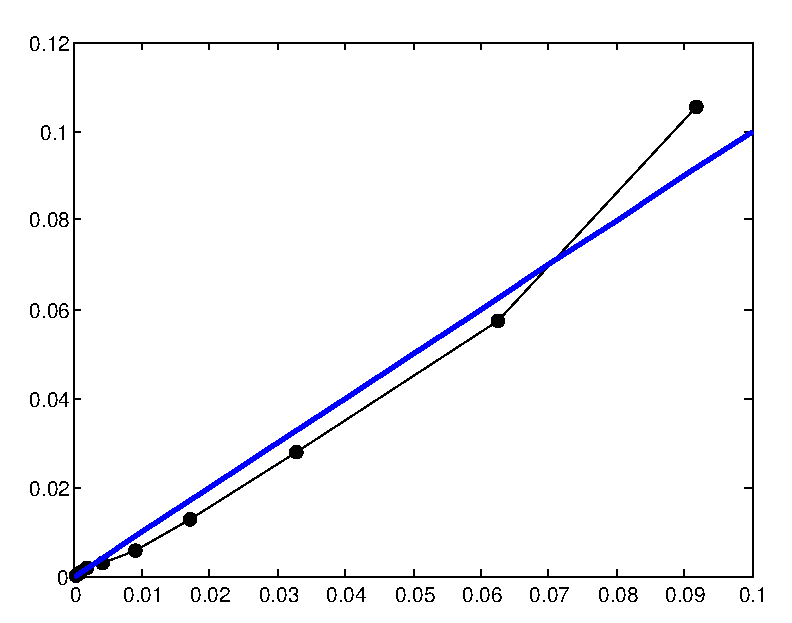
\includegraphics[width=0.7\textwidth]{images/lect12b_cropped.pdf}
 \caption{Trajectory and central path in $x_2s_2-x_5s_5$ coordinates.}\label{fig:fig2}
\end{figure}

\section{Analysis of Path-following}
In the analysis of the long-step path-following algorithm, it is enough to establish that the duality measure $\mu^{(k)}$ converges to $0$ as $k\to \infty$. The reason is that $\mu=0$ forces all the products $x_is_i=0$, and since by design the other constraints are satisfied, this means that the sequence of points converges to a solution. The first theorem tells us that the $\mu_k$ decrease as $k$ increases. An elementary proof is given in Theorem 14.3 in Nocedal and Wright. It depends crucially on the assumption that the iterates remain inside the neighbourhood $\mathcal{N}_{-\infty}(\gamma)$ of the central path.

\begin{theorem}
 Given parameters $\gamma$, $\sigma_{\mathrm{min}}$ and $\sigma_{\mathrm{max}}$, there is a constant $\delta>0$, independent of $n$, such that
 \begin{equation}\label{thm:1}
  \mu_{k+1}\leq \left(1-\frac{\delta}{n}\right) \mu_k.
 \end{equation}
\end{theorem}

The next theorem gives a bound on the number of iterations needed to reduce the duality measure beyond any given $\e$.

\begin{theorem}
 Let $\e>0$ and $\gamma\in (0,1)$. Let $(\vct{x}^{(0)},\vct{y}^{(0)},\vct{s}^{(0)})\in \mathcal{N}_{-\infty}(\gamma)$ be a starting point such that the duality measure satisfies $\mu^{(0)}\leq \e^{-\kappa}$ for some constant $\kappa$. Then there is an index $K=O(n\log (1/\e))$ such that for all $k>K$,
 \begin{equation*}
  \mu_k \leq \e.
 \end{equation*}
In particular, the long-step path-following algorithm converges.
\end{theorem}

\begin{proof}
Repeatedly applying~\eqref{thm:1}, we get
\begin{equation*}
 \mu_{k} \leq \left(1-\frac{\delta}{n}\right)^k \mu_0.
\end{equation*}
Taking logarithms on both sides,
 \begin{align*}
  \log \mu_{k}\leq k \log\left(1-\frac{\delta}{n}\right)+\log \mu_0 
  &\leq k \log\left(1-\frac{\delta}{n}\right)+\kappa \log\left(\frac{1}{\e}\right)\\
  &\leq k\frac{-\delta}{n}+\kappa\log\left(\frac{1}{\e}\right).
 \end{align*}
We have $\mu_k<\e$ if 
\begin{equation*}
 -k\frac{\delta}{n}+\kappa \left(\frac{1}{\e}\right) \leq \log \e,
\end{equation*}
of equivalently, if 
\begin{equation*}
 k\geq (1+\kappa)\frac{n}{\delta}\log\left(\frac{1}{\e}\right)=K.
\end{equation*}
This was to be shown.

\end{proof}



% %-----------------------------------------------------------------------
% % End of chap1.tex
% %-----------------------------------------------------------------------

\part{Non-linear Convex Optimization}
%-----------------------------------------------------------------------
% Beginning of chap2.tex
%-----------------------------------------------------------------------
%
%  AMS-LaTeX sample file for a chapter of a monograph, to be used with
%  an AMS monograph document class.  This is a data file input by
%  chapter.tex.
%
%  Use this file as a model for a chapter; DO NOT START BY removing its
%  contents and filling in your own text.
% 
%%%%%%%%%%%%%%%%%%%%%%%%%%%%%%%%%%%%%%%%%%%%%%%%%%%%%%%%%%%%%%%%%%%%%%%%


\chapter*{Lecture 14}
\addcontentsline{toc}{chapter}{Lecture 14}
\addtocounter{chapter}{14}
%\addtocounter{section}{-2}
%\numberwithin{section}{chapter}
\numberwithin{equation}{chapter}
\numberwithin{theorem}{chapter}

%\epigraph{}{--- \textup{}}

So far we have only dealt with constrained optimization problems where the objective and the constraints are linear. We now turn attention to general problems of the form

\begin{align*}\label{eq:constr}\tag{1}
\begin{split}
 \minimize & f(\vct{x})\\
 \subjto & \vct{g}(\vct{x})\leq \zerovct\\
         & \vct{h}(\vct{x})= \zerovct,
\end{split}
\end{align*}
where $\vct{x}\in \R^n$, $\vct{g}=(g_1,\dots,g_m)^{\trans}$, $\vct{g}=(g_1,\dots,g_{\ell})$, and the inequalities are componentwise. 
The problem~\eqref{eq:constr} is {\em convex}, if $f$ and the $g_i$ are convex, and the $h_j$ are linear. We also denote by $\mathrm{dom}(f)$ the {\em domain} of $f$, which is the set of points $\vct{x}$ where $f$ takes a finite value. The feasible set
\begin{equation*}
 \mathcal{F} = \{\vct{x} \mid g_i(\vct{x})\leq 0, \ h_j(\vct{x})=0, \ 1\leq i\leq m, \ 1\leq j\leq \ell\}
\end{equation*}
for a convex constrained problem is a convex set.

\section{Quadratic Programming and Portfolio Optimization}
The simplest case of non-linear, constrained convex optimization is \textbf{quadratic programming}. Quadratic programming problems are of the form
\begin{align*}
  \minimize & \frac{1}{2}\vct{x}^{\trans}\mtx{Q}\vct{x}+\vct{c}^{\trans}\vct{x}\\
  \subjto & \mtx{A}\vct{x}\leq \vct{b},
\end{align*}
with $\mtx{Q}$ symmetric and positive semidefinite.
Note that this problem combines two problems we studied in some detail before: minimizing a quadratic function, and linear constraints. Just as we did for unconstrained minimization and for linear programming, we will derive optimality conditions for such problems. Before studying the theory, we first present an important application: portfolio optimization.

\subsection{Mean-variance portfolio theory}
If we invest an amount $x^0$ into a product at period $0$, and at period $1$ (for example, one day) the value is $x^1$, then the \textbf{relative return} is defined as
\begin{equation*}
  r = \frac{x^{1}-x^{0}}{x^{0}}.
\end{equation*}

The following figure shows the price movement and the returns of a stock from January 2016 until now.

\begin{figure}
\centering
\includegraphics[width=0.8\textwidth]{images/stock.png}
\end{figure}

As we can't predict the future, we usually work with the \textbf{expected return} $\mtx{E}[r]=\mu$, which is a statistical estimate of the future return. One naive method of estimating the future return is by taking the average of past returns, but other more sophisticated methods are possible.

In \textbf{portfolio optimization}, we have a proportion $x_i$ of our available funds that we want to invest in a stock $i$ (in particular, as $x_i$ measures a proportion, we have $\sum_{i=1}^n x_i = 1$). We may or may not allow $x_i<0$, which would correspond to short-selling or borrowing. Given this allocation, the overall return is $\vct{x}^{\trans}\vct{r}$, where $\vct{x}=(x_1,\dots,x_n)^{\trans}$ and $\vct{r}=(r_1,\dots,r_n)^{\trans}$ is the vector of (relative) returns.
If $\vct{\mu}=\mtx{E}[\vct{r}]$ denotes the vector of expected returns, then the total expected return is 
\begin{equation*}
\mu = \vct{x}^{\trans}\vct{\mu}=\sum_{i=1}^n x_i\mu_i.
\end{equation*} 
 The \textbf{risk} is an investment is measured in terms of the \textbf{variance} of the returns $r=\vct{x}^{\trans}\vct{r}$. Let $\mtx{\Sigma}$ denote the \textbf{covariance matrix}, where the $(i,j)$-th entry is $\mathrm{Cov}(r_i,r_j) = \mtx{E}[(r_i-\mu_i)(r_j-\mu_j)]$. The $(i,j)$-th entry measures how much products $i$ and $j$ are correlated. The \textbf{variance} of the returns $r$ is then the quadratic function
 \begin{equation*}
   \vct{x}^{\trans}\Sigma\vct{x}.
 \end{equation*} 
  
A portfolio optimization problem either seeks to maximize the return while bounding the risk,
 \begin{align*}
  \maximize & \vct{x}^{\trans}\vct{\mu}\\
  \subjto & \vct{x}^{\trans}\mtx{\Sigma}\vct{x}\leq \sigma,\\
  & \sum_{i=1}^n x_i=1\\
  & x_i\geq 0,
 \end{align*}
or minimize the risk given a certain target return $\mu$,
\begin{align*}
 \minimize & \vct{x}^{\trans}\mtx{\Sigma}\vct{x}\\
 \subjto & \vct{x}^{\trans}\vct{\mu} = \mu\\
 & \sum_{i=1}^n x_i = 1\\
 & x_i\geq 0.
\end{align*}

Both of these problems are convex optimization problems. The constraints $x_i\geq 0$ mean that we are not allowed to short-sell; when dealing with futures or options, or if we are a large institutional investor, we may drop these constraints. As we will see later, dropping the inequality constraints from the second formulation allows the problem to be solved in closed form.

A third form of the portfolio optimization problem is to combine the expected return and the risk into a single objective function, as follows:
\begin{align*}
 \maximize & \vct{\mu}^{\trans}\vct{x} - \gamma \vct{x}^{\trans}\mtx{\Sigma}\vct{x}\\
 \subjto & \sum_{i=1}^n x_i = 1\\
 & x_i\geq 0.
\end{align*}
Note that this is a convex quadratic problem: we can transform it into a minimization problem with the matrix $\mtx{\Sigma}$ by changing the sign.
The parameter $\gamma$ is called a \textbf{risk aversion parameter}; it adjusts the level of risk we are willing to take. If $\gamma=0$, then the quadratic term does not feature in the objective and we just aim to maximize the expected return. If $\gamma$ is big, then the risk term weighs heavily on the objective function, and the optimal value will like be one where $\vct{x}^{\trans}\mtx{\Sigma}\vct{x}$ is small. By varying the value of $\gamma$, we get different expected return / risk (variance) trade-offs. The following code computes this trade-off curve for a portfolio of $10$ stock from the FT100 index. The mean and covariance where computing by averaging over the past 60 trading days (3 months). The $x$-axis is the \textbf{standard deviation}, which is given as the square root of the variance (risk). 

\begin{ipythonnb}
from datetime import datetime, date
import pandas as pd
from pandas_datareader import data, wb
import numpy as np
import matplotlib.pyplot as plt
from cvxpy import *
\end{ipythonnb}

We first use the functionality of the Pandas module to load the price data from the Yahoo Finance web site. 

\begin{ipythonnb}
START = datetime(2016,1,1)
END = date.today()
TICKER = ['ADN', 'AZN', 'EZJ', 'GSK', 'ITV', 'LSE', 'TSCO', 'PSON', 'PRU', 'DGE']
mydata = data.DataReader('TSCO', "yahoo", START, END)
dates = mydata.index
df = pd.DataFrame(index=dates, columns=TICKER)
for x in TICKER:
    mydata = data.DataReader(x, "yahoo", START, END)
    df.loc[:,x] = mydata['Adj Close']
df = df.dropna()
df.head(2)
\end{ipythonnb}

The following shows a small sample of the data loaded.

\begin{tabular}{lcccccccccc}
 	   & ADN & AZN & EZJ & GSK & ITV & LSE & TSCO \\
Date & & & & & & & & & & \\ 										
2016-01-04 & 2.41197 & 31.926706 & 84.900002 & 37.813187 & 0.4 & 0.002 & 82.800593 \\
2016-01-05 & 2.41197 & 32.404650 & 86.620003 & 38.028194 & 0.4 & 0.001 & 82.741275 \\
\end{tabular}

We next compute the returns and the mean and covariance.

\begin{ipythonnb}
price_matrix = df.values
returns = (price_matrix[1:]-price_matrix[0:-1])/price_matrix[0:-1]
mu = np.mean(returns[-60:,:], axis=0)
Sigma = np.cov(returns[-60:,:].T)
n = 10
\end{ipythonnb}

In the next step, we start the CVXPY engine and compute the mean-variance trade-off curve. We include the constraint $\vct{x}\geq 0$ to disallow for short-selling.

\begin{ipythonnb}
x = Variable(n)
gamma = Parameter(sign='positive')
ret = mu.T*x
risk = quad_form(x, Sigma)
prob = Problem(Maximize(ret - gamma*risk), 
               [sum_entries(x) == 1, 
                x >= 0])
\end{ipythonnb}

\begin{ipythonnb}
SAMPLES = 1000
risk_data = np.zeros(SAMPLES)
ret_data = np.zeros(SAMPLES)
gamma_vals = np.logspace(-2, 3, num=SAMPLES)
for i in range(SAMPLES):
    gamma.value = gamma_vals[i]
    prob.solve()
    risk_data[i] = sqrt(risk).value
    ret_data[i] = ret.value
\end{ipythonnb}

\begin{ipythonnb}
markers_on = [290, 400]
fig = plt.figure()
ax = fig.add_subplot(111)
plt.plot(risk_data, ret_data, 'g-')
for marker in markers_on:
    plt.plot(risk_data[marker], ret_data[marker], 'bs')
    ax.annotate(r"$\gamma = %.2f$" 
    % gamma_vals[marker], xy=(risk_data[marker]+0.01, ret_data[marker]-0.01))
for i in range(n):
    plt.plot(sqrt(Sigma[i,i]).value, mu[i], 'ro')
plt.xlabel('Standard deviation')
plt.ylabel('Return')
plt.show()
\end{ipythonnb}

\begin{figure}
\centering
\includegraphics[width=0.8\textwidth]{images/meanvar.png}
\end{figure}

The red dots represent the standard deviation and expected return of the individual stocks. The two blue dots indicate the standard deviation and expected return of the portfolio for two values of $\gamma$. Which value of $\gamma$ we go for depends on how much risk we are willing to take: if we are risk-averse, we may prefer the $\gamma=1$ value to the $\gamma=0.028$ value, at the expense of smaller expected returns.

In practical applications there are a lot of other factors to be considered, such as whether the estimation procedure for the mean and covariance makes sense. In addition, it is often common to add terms that account for \textbf{transaction costs} into the objective funtion.

%\begin{remark}
% There are many problems of interest which are not convex, but in some cases it is possible to formulate an {\em equivalent} convex optimization problem. For example, consider the optimization problem
% \begin{equation}\label{eq:ex1}
%  \minimize x_1^2+x_2^2 \quad \subjto \frac{x_1}{1+x_2^2}\leq 0, \ (x_1+x_2)^2=0.
% \end{equation}
%This problem is not a convex optimization problem (why?). However, the following problem
%\begin{equation}\label{eq:ex2}
% \minimize x_1^2+x_2^2 \quad \subjto x_1\leq 0, \ x_1+x_2=0
%\end{equation}
%is clearly convex, and the solution of~\eqref{eq:ex1} coincides with the solution of~\eqref{eq:ex2}.
%\end{remark}
%
%\section{First order optimality conditions}
%So far we have seen two examples of first order optimality conditions: for unconstraint optimization ($\nabla f(\vct{x})=0$) and for linear programming. We now generalize these to the setting of constrained convex optimization.
%
%\begin{theorem}
% Let $f\colon \R^d\to \R$ be a convex, differentiable function, and 
% \begin{equation*}
%  \mathcal{F}=\{\vct{x} \mid g_i(\vct{x})\leq 0, \ h_j(\vct{x})=0, \ 1\leq i\leq m, \ 1\leq j\leq \ell\}
% \end{equation*}
%a feasible set, with $g_i$ convex and $h_j$ linear. Then $\vct{x}^*$ is an optimal point of the optimization problem
%\begin{equation*}
% \minimize f(\vct{x}) \ \subjto \vct{x}\in \mathcal{F}
%\end{equation*}
%if and only if for all $\vct{y}\in \mathcal{F}$, 
%\begin{equation}\label{eq:opt}
% \ip{\nabla f(\vct{x}^*)}{\vct{y}-\vct{x}^*}\geq 0.
%\end{equation}
%\end{theorem}
%
%\begin{proof}
% Suppose $\vct{x}^*$ is such that~\eqref{eq:constr} holds. Then, since $f$ is a convex function,
% for all $\vct{y}\in \mathcal{F}$ we have, by Theorem 2.4.1,
% \begin{equation*}
%  f(\vct{y})\geq f(\vct{x}^*)+\ip{\nabla f(\vct{x}^*)}{\vct{y}-\vct{x}^*} \geq f(\vct{x}^*),
% \end{equation*}
%which shows that $\vct{x}^*$ is a minimizer in $\mathcal{F}$. To show the opposite direction, assume that $\vct{x}^*$ is a minimizer but that~\eqref{eq:constr} does not hold. This means that there exists a $\vct{y}\in \mathcal{F}$ such that $\ip{\nabla f(\vct{x}^*)}{\vct{y}-\vct{x}^*}<0$. Since both $\vct{x}^*$ and $\vct{y}$ are in $\mathcal{F}$ and $\mathcal{F}$ is convex, any point $\vct{z}(\lambda)=(1-\lambda)\vct{x}^*+t\vct{y}$ with $\lambda\in [0,1]$ is also in $\mathcal{F}$. At $\lambda=0$ we have
%\begin{equation*}
% \frac{df}{d\lambda}f(\vct{z}(\lambda))|_{\lambda=0} = \ip{\nabla f(\vct{x}^*)}{\vct{y}-\vct{x}^*}<0.
%\end{equation*}
%Since the derivative at $\lambda=0$ is negative, the function $f(\vct{z}(\lambda))$ is decreasing at $\lambda=0$, and therefore, for small $\lambda>0$, $f(\vct{z}(\lambda))<f(\vct{z}(0))=f(\vct{x}^*)$, in contradiction to the assumption that $\vct{x}^*$ is a minimizer.
%\end{proof}
%
%\begin{example}
% In the absence of constraints, $\mathcal{F}=\R^d$, and the statement says that
% \begin{equation*}
%  \forall \vct{y}\in \R^d\colon \ip{\nabla f(\vct{x}^*)}{\vct{y}-\vct{x}^*}\geq 0.
% \end{equation*}
%If there was a $\vct{y}$ such that $\ip{\nabla f(\vct{x}^*)}{\vct{y}-\vct{x}^*}>0$, then replacing $\vct{y}$ by $2\vct{x}-\vct{y}$ we also have the converse inequality, and therefore the optimality condition is equivalent to saying that $\nabla f(\vct{x}^*)=\zerovct$. We therefore recover the well-known first order optimality condition from Lecture 2. 
%\end{example}
%
%Geometrically, the first order optimality condition means that the set
%\begin{equation*}
% \{\vct{x}\mid \ip{\nabla f(\vct{x}^*)}{\vct{x}}=\ip{\nabla f(\vct{x}^*)}{\vct{x}^*}\}
%\end{equation*}
%defines a supporting hyperplane to the set $\mathcal{F}$.
%
%\begin{figure}[h!]
%\centering
%\begin{tikzpicture}[thick,rotate=30,scale=0.8]
%\filldraw[color=black, fill=blue!5, very thick](0,0) ellipse (2 and 1.2);
%\node (A1) at (0,-3)  [label=0:{$-\nabla f(\vct{x}^*)$}] {};
%\node (A2) at (0,-1.2)  [label=90:{$\vct{x}^*$}] {};
%%\node (A3) at (0,-2.5)  [label=180:{$\vct{a}$}] {};
%\node (A4) at (-1,0)  [label=180:{$\vct{y}$}] {};
%\filldraw[black] (0,-3) circle (2pt);
%\filldraw[black] (0,-1.2) circle (2pt);
%\filldraw[black] (-1,0) circle (2pt);
%\draw[color=black, thick, <-] (0,-2.9) -- (0,-1.2);
%\draw[color=black, thick, <-] (-0.9,-0.1) -- (0,-1.2);
%\end{tikzpicture}
%\caption{Optimality condition} \label{fig:neg}
%\end{figure}

% %-----------------------------------------------------------------------
% % End of chap1.tex
% %-----------------------------------------------------------------------

%-----------------------------------------------------------------------
% Beginning of chap2.tex
%-----------------------------------------------------------------------
%
%  AMS-LaTeX sample file for a chapter of a monograph, to be used with
%  an AMS monograph document class.  This is a data file input by
%  chapter.tex.
%
%  Use this file as a model for a chapter; DO NOT START BY removing its
%  contents and filling in your own text.
% 
%%%%%%%%%%%%%%%%%%%%%%%%%%%%%%%%%%%%%%%%%%%%%%%%%%%%%%%%%%%%%%%%%%%%%%%%


\chapter*{Lecture 15}
\addcontentsline{toc}{chapter}{Lecture 15}
\addtocounter{chapter}{15}
\addtocounter{section}{0}
%\numberwithin{section}{chapter}
\numberwithin{equation}{chapter}
\numberwithin{theorem}{chapter}

%\epigraph{}{--- \textup{}}

In this lecture we study optimality conditions for convex problems of the form

\begin{align*}\label{eq:constr}\tag{1}
\begin{split}
 \minimize & f(\vct{x})\\
 \subjto & \vct{f}(\vct{x})\leq \zerovct\\
         & \vct{h}(\vct{x})= \zerovct,
\end{split}
\end{align*}
where $\vct{x}\in \R^n$, $\vct{f}=(f_1,\dots,f_m)^{\trans}$, $\vct{h}=(h_1,\dots,h_p)^{\trans}$, and the inequalities are componentwise. We assume that $f$ and the $f_i$ are convex, and the $h_j$ are linear. It is also customary to write the conditions $\vct{h}(\vct{x})=\zerovct$ as $\mtx{A}\vct{x}=\vct{b}$, with $h_j(\vct{x}) = \vct{a}_j^{\trans}\vct{x}-b_j$, $\vct{a}_j$ being the $j$-th row of $\mtx{A}$.

\section{A first-order optimality condition}
So far we have seen two examples of first order optimality conditions: for unconstraint optimization ($\nabla f(\vct{x})=0$) and for linear programming. We now generalize these to the setting of constrained convex optimization.

\begin{theorem}
 Let $f\colon \R^n\to \R$ be a convex, differentiable function, and 
 \begin{equation*}
  \mathcal{F}=\{\vct{x} \mid f_i(\vct{x})\leq 0, \ \mtx{A}\vct{x}=\vct{b}\}
 \end{equation*}
a feasible set, with $f_i$ convex. Then $\vct{x}^*$ is an optimal point of the optimization problem
\begin{equation*}
 \minimize f(\vct{x}) \ \subjto \vct{x}\in \mathcal{F}
\end{equation*}
if and only if for all $\vct{y}\in \mathcal{F}$, 
\begin{equation}\label{eq:opt}
 \ip{\nabla f(\vct{x}^*)}{\vct{y}-\vct{x}^*}\geq 0.
\end{equation}
\end{theorem}

\begin{proof}
 Suppose $\vct{x}^*$ is such that~\eqref{eq:constr} holds. Then, since $f$ is a convex function,
 for all $\vct{y}\in \mathcal{F}$ we have, by Theorem 2.10.1,
 \begin{equation*}
  f(\vct{y})\geq f(\vct{x}^*)+\ip{\nabla f(\vct{x}^*)}{\vct{y}-\vct{x}^*} \geq f(\vct{x}^*),
 \end{equation*}
which shows that $\vct{x}^*$ is a minimizer in $\mathcal{F}$. To show the opposite direction, assume that $\vct{x}^*$ is a minimizer but that~\eqref{eq:constr} does not hold. This means that there exists a $\vct{y}\in \mathcal{F}$ such that $\ip{\nabla f(\vct{x}^*)}{\vct{y}-\vct{x}^*}<0$. Since both $\vct{x}^*$ and $\vct{y}$ are in $\mathcal{F}$ and $\mathcal{F}$ is convex, any point $\vct{z}(\lambda)=(1-\lambda)\vct{x}^*+\lambda\vct{y}$ with $\lambda\in [0,1]$ is also in $\mathcal{F}$. At $\lambda=0$ we have
\begin{equation*}
 \frac{df}{d\lambda}f(\vct{z}(\lambda))|_{\lambda=0} = \ip{\nabla f(\vct{x}^*)}{\vct{y}-\vct{x}^*}<0.
\end{equation*}
Since the derivative at $\lambda=0$ is negative, the function $f(\vct{z}(\lambda))$ is decreasing at $\lambda=0$, and therefore, for small $\lambda>0$, $f(\vct{z}(\lambda))<f(\vct{z}(0))=f(\vct{x}^*)$, in contradiction to the assumption that $\vct{x}^*$ is a minimizer.
\end{proof}

\begin{example}
 In the absence of constraints, $\mathcal{F}=\R^n$, and the statement says that
 \begin{equation*}
  \forall \vct{y}\in \R^n\colon \ip{\nabla f(\vct{x}^*)}{\vct{y}-\vct{x}^*}\geq 0.
 \end{equation*}
Given $\vct{y}$ such that $\ip{\nabla f(\vct{x}^*)}{\vct{y}-\vct{x}^*}\geq 0$, then replacing $\vct{y}$ by $2\vct{x}-\vct{y}$ we also have the converse inequality, and therefore the optimality condition is equivalent to saying that $\nabla f(\vct{x}^*)=\zerovct$. We therefore recover the well-known first order optimality condition from Lecture 2. 
\end{example}

Geometrically, the first order optimality condition means that the set
\begin{equation*}
 \{\vct{x}\mid \ip{\nabla f(\vct{x}^*)}{\vct{x}}=\ip{\nabla f(\vct{x}^*)}{\vct{x}^*}\}
\end{equation*}
defines a supporting hyperplane to the set $\mathcal{F}$.

\begin{figure}[h!]
\centering
\begin{tikzpicture}[thick,rotate=30,scale=0.8]
\filldraw[color=black, fill=blue!5, very thick](0,0) ellipse (2 and 1.2);
\node (A1) at (0,-3)  [label=0:{$-\nabla f(\vct{x}^*)$}] {};
\node (A2) at (0,-1.2)  [label=90:{$\vct{x}^*$}] {};
%\node (A3) at (0,-2.5)  [label=180:{$\vct{a}$}] {};
\node (A4) at (-1,0)  [label=180:{$\vct{y}$}] {};
\filldraw[black] (0,-3) circle (2pt);
\filldraw[black] (0,-1.2) circle (2pt);
\filldraw[black] (-1,0) circle (2pt);
\draw[color=black, thick, <-] (0,-2.9) -- (0,-1.2);
\draw[color=black, thick, <-] (-0.9,-0.1) -- (0,-1.2);
\end{tikzpicture}
\caption{Optimality condition} \label{fig:neg}
\end{figure}

\section{Lagrangian duality}
Recall the method of Lagrange multipliers. Given two functions $f(x,y)$ and $h(x,y)$, if the problem
\begin{equation*}
 \minimize f(x,y) \quad \subjto h(x,y)=0
\end{equation*}
has a solution $(x^*,y^*)$, then there exists a parameter $\lambda$, the {\em Lagrange multiplier}, such that
\begin{equation}\label{eq:lag}
 \nabla f(x^*,y^*) = \lambda \nabla h(x^*,y^*).
\end{equation}
In other words, if we define the {\em Lagrangian} as 
\begin{equation*}
 \mathcal{L}(x,y,\lambda) = f(x,y)-\lambda h(x,y),
\end{equation*}
then~\eqref{eq:lag} says that $\nabla \mathcal{L}(x^*,y^*,\lambda) = 0$ for some $\lambda$. The intuition is as follows. The set
\begin{equation*}
 M = \{(x,y)\in \R^2 \mid h(x,y)=0\}
\end{equation*}
is a curve in $\R^2$, and the gradient $\nabla h(x,y)$ is perpendicular to $M$ at every point $(x,y)\in M$. For someone living inside $M$, a vector that is perpendicular to $M$ is not visible, it is zero. Therefore the gradient $\nabla f(x,y)$ is zero as viewed from within $M$ if it is perpendicular to $M$, or equivalently, a multiple of $\nabla h(x,y)$.


Alternatively, we can view the graph of $f(x,y)$ in three dimensions. A maximum or minimum of $f(x,y)$ along the curve defined by $h(x,y)=0$ will be a point at which the direction of steepest ascent $\nabla f(x,y)$ is perpendicular to the curve $h(x,y)=0$.

\begin{example}
 Consider the function $f(x,y)=x^2y$ with the constraint $h(x,y)=x^2+y^2-3$ (a circle of radius $\sqrt{3}$). The Lagrangian is the function
 \begin{equation*}
  \mathcal{L}(x,y,\lambda) = x^2y-\lambda(x^2+y^2-3).
 \end{equation*}
Computing the partial derivatives gives the three equations
\begin{align*}
\frac{\partial}{\partial x} \mathcal{L} &= 2xy-2\lambda x = 0\\
\frac{\partial}{\partial y} \mathcal{L} &= x^2-2\lambda y = 0\\
\frac{\partial}{\partial \lambda} \mathcal{L} &= x^2+y^2-3 = 0.
\end{align*}
From the second equation we get $\lambda = \frac{x^2}{2y}$,
and the first and third equations become
\begin{align*}
 2xy-\frac{x^3}{y} &= 0\\
 x^2+y^2-3&=0.
\end{align*}
Solving this system, we get six critical point $(\pm \sqrt{2},\pm 1)$, $(0,\pm \sqrt{2})$. To find out which one of these is the minimizers, we just evaluate the function $f$ on each of these.
\end{example}


We now turn to convex problems of the more general form form
\begin{align}\label{eq:sys1}
\begin{split}
 \minimize & f(\vct{x})\\
 \subjto & \vct{f}(\vct{x})\leq \zerovct\\
         & \vct{h}(\vct{x})= \zerovct,
\end{split}
\end{align}
Denote by $\mathcal{D}$ the {\em domain} of all the functions $f,f_i,h_j$, i.e., 
\begin{equation*}
 \mathcal{D} = \mathrm{dom}(f)\cap \mathrm{dom}(f_1)\cap\cdots\cap\mathrm{dom}(f_m)\cap \mathrm{dom}(h_1)\cap\cdots \cap \mathrm{dom}(h_p).
\end{equation*}
Assume that $\mathcal{D}$ is not empty and let $p^*$ be the optimal value of~\eqref{eq:sys1}.

The {\em Lagrangian} of the system is defined as
\begin{equation*}
 \mathcal{L}(\vct{x},\vct{\lambda},\vct{\mu}) = f(\vct{x})+\vct{\lambda}^{\trans}\vct{f}(\vct{x})+\vct{\mu}^{\trans}h(\vct{x}) = f(\vct{x}) +\sum_{i=1}^m \lambda_i f_i(\vct{x})+\sum_{i=1}^p \mu_i h_i(\vct{x}).
\end{equation*}
The vectors $\vct{\lambda}$ and $\vct{\mu}$ are called the {\em dual variables} or {\em Lagrange multipliers} of the system. The domain of $\mathcal{L}$ is $\mathcal{D}\times \R^m\times \R^{p}$. 

\begin{definition}
 The {\em Lagrange dual} of the problem~\eqref{eq:sys1} is the function
 \begin{equation*}
  g(\vct{\lambda},\vct{\mu}) = \inf_{\vct{x}\in \mathcal{D}} \mathcal{L}(\vct{x},\vct{\lambda},\vct{\mu}).
 \end{equation*}
If the Lagrangian $\mathcal{L}$ is unbounded from below, then the value is $-\infty$.
\end{definition}

The Lagrangian $\mathcal{L}$ is linear in the $\lambda_i$ and $\mu_j$ variables. The infimum of a family of linear functions is concave, so that the Lagrange dual is a concave function. Therefore the negative $-g(\vct{\lambda},\vct{\mu})$ is a convex function.

\begin{lemma}\label{le:lag1}
 For any $\vct{\mu}\in \R^{p}$ and $\vct{\lambda}\geq \zerovct$ we have
 \begin{equation*}
 g(\vct{\lambda},\vct{\mu})\leq p^*.
 \end{equation*}
\end{lemma}

\begin{proof}
 Let $\vct{x}^*$ be a feasible point for~\eqref{eq:sys1}, that is,
 \begin{equation*}
  f_i(\vct{x}^*)\leq 0, \quad h_j(\vct{x}^*)=0,\ 1\leq i\leq m, \ 1\leq j\leq p.
 \end{equation*}
Then for $\vct{\lambda}\geq \zerovct$ and any $\vct{\mu}$, since each $h_j(\vct{x}^*)=0$ and $\lambda_jf_j(\vct{x}^*)\leq 0$, 
\begin{equation*}
 \mathcal{L}(\vct{x}^*,\vct{\lambda},\vct{\mu}) = f(\vct{x}^*)+\sum_{i=1}^m \lambda_if_i(\vct{x}^*)+\sum_{j=1}^p \mu_j h_j(\vct{x}^*)\leq f(\vct{x}^*).
\end{equation*}
In particular,
\begin{equation*}
 g(\vct{\lambda},\vct{\mu}) = \inf_{\vct{x}} \mathcal{L}(\vct{x},\vct{\lambda},\vct{\mu}) \leq \mathcal{L}(\vct{x}^*,\vct{\lambda},\vct{\mu}) \leq f(\vct{x}^*).
\end{equation*}
Since this holds for {\em all} feasible $\vct{x}^*$, it holds in particular for the $\vct{x}^*$ that minimizes~\eqref{eq:sys1}, for which $f(\vct{x}^*)=p^*$. 
\end{proof}

A point $(\vct{\lambda},\vct{\mu})$ with $\vct{\lambda}\geq \zerovct$ and $(\vct{\lambda},\vct{\mu})\in \mathrm{dom}(g)$ is called a {\em feasible point} of the dual problem.

The {\em Lagrange dual} of the optimization problem~\eqref{eq:sys1} is the problem
\begin{equation}\label{eq:lagdual}
 \maximize g(\vct{\lambda},\vct{\mu}) \quad \subjto \vct{\lambda}\geq \zerovct.
\end{equation}
We have seen that if $q^*$ is the optimal value of~\eqref{eq:lagdual}, then $q^*\leq p^*$, and the example above implies that in the special case of linear programming we actually have $q^*=p^*$. We will see that under certain conditions, we have $q^*=p^*$ for more general problems, but this is not always the case.


% %-----------------------------------------------------------------------
% % End of chap1.tex
% %-----------------------------------------------------------------------

%-----------------------------------------------------------------------
% Beginning of chap2.tex
%-----------------------------------------------------------------------
%
%  AMS-LaTeX sample file for a chapter of a monograph, to be used with
%  an AMS monograph document class.  This is a data file input by
%  chapter.tex.
%
%  Use this file as a model for a chapter; DO NOT START BY removing its
%  contents and filling in your own text.
% 
%%%%%%%%%%%%%%%%%%%%%%%%%%%%%%%%%%%%%%%%%%%%%%%%%%%%%%%%%%%%%%%%%%%%%%%%


\chapter*{Lecture 16}
\addcontentsline{toc}{chapter}{Lecture 16}
\addtocounter{chapter}{16}
\addtocounter{section}{0}
%\numberwithin{section}{chapter}
\numberwithin{equation}{chapter}
\numberwithin{theorem}{chapter}
%\epigraph{}{--- \textup{}}

For convex problems of the form

\begin{align*}\label{eq:constr}\tag{1}
\begin{split}
 \minimize & f(\vct{x})\\
 \subjto & \vct{f}(\vct{x})\leq \zerovct\\
         & \mtx{A}\vct{x} = \vct{b},
\end{split}
\end{align*}
we introduced the Lagrangian $\mathcal{L}(\vct{x},\vct{\lambda},\vct{\mu})$ and defined the Lagrange dual as
\begin{equation*}
 g(\vct{\lambda},\vct{\mu})=\inf_{\vct{x}\in \mathcal{D}} \mathcal{L}(\vct{x},\vct{\lambda},\vct{\mu}).
\end{equation*}
We saw that $g(\vct{\lambda},\vct{\mu})$ is a lower bound on the optimal value of~\eqref{eq:constr}. Note that here we wrote the conditions $h_j(\vct{x})=0$ as system of linear equations $\mtx{A}\vct{x}=\vct{b}$, since for the problem to be convex, we require that the $h_j$ be linear functions.

\begin{example}
 Consider a linear programming problem of the form
 \begin{align*}
  \minimize & \ip{\vct{c}}{\vct{x}}\\
  \subjto & \mtx{A}\vct{x}=\vct{b}\\
  & \vct{x}\geq \zerovct.
 \end{align*}
The inequality constraints are $-x_i\leq 0$, while the equality constraints are $\vct{a}_i^{\trans}\vct{x}-b_i$. The Lagrangian has the form
\begin{align*}
 \mathcal{L}(\vct{x},\vct{\lambda},\vct{\mu}) &= \ip{\vct{c}}{\vct{x}}-\sum_{i=1}^n \lambda_i x_i + \sum_{j=1}^m \mu_j(\vct{a}_j^{\trans}\vct{x}-b_j)\\
 &= (\vct{c}-\vct{\lambda}+\mtx{A}^{\trans}\vct{\mu})^{\trans}\vct{x}-\vct{b}^{\trans}\vct{\mu}.
\end{align*}
The infimum over $\vct{x}$ of this function is $-\infty$ unless $\vct{c}-\vct{\lambda}+\mtx{A}^{\trans}\vct{\mu}= \zerovct$. The Lagrange dual is therefore
\begin{equation*}
 g(\vct{\lambda},\vct{\mu}) = \begin{cases} 
                               -\vct{\mu}^{\trans}\vct{b} & \text{ if } \vct{c}-\vct{\lambda}+\mtx{A}^{\trans}\vct{\mu}=\zerovct\\
                               -\infty & \text{ else.}
                              \end{cases}
\end{equation*}
From Lemma 15.5 we conclude that
\begin{equation*}
 \max \{-\vct{b}^{\trans}\vct{\mu} \mid \vct{c}-\vct{\lambda}+\mtx{A}^{\trans}\vct{\mu}=\zerovct, \ \vct{\lambda}\geq \zerovct\} \leq \min \{\vct{c}^{\trans}\vct{x} \mid \mtx{A}\vct{x}=\zerovct, \ \vct{x}\geq \zerovct\}.
\end{equation*}
Note that if we write $\vct{y}=-\vct{\mu}$ and $\vct{s}=\vct{\lambda}$, then we get the dual version of the linear programming problem we started out with, and in this case we know that 
\begin{equation*}
 \max_{\vct{\lambda}\geq \zerovct,\vct{\mu}} g(\vct{\lambda},\vct{\mu}) = p^*.
\end{equation*}
\end{example}


\section{Constraint qualification}
In the example of linear programming, we have seen that the optimal value of the dual problem is equal to the optimal value of the primal problem. In general, we have
\begin{equation*}
 d^* = \sup_{\vct{\lambda}>0,\vct{\mu}} g(\vct{\lambda},\vct{\mu}) \leq \inf_{\vct{x}\in \mathcal{D}} \{f(\vct{x}) \mid f_i(\vct{x})\leq 0, \ \mtx{A}\vct{x}=\vct{b}\}=p^*.
\end{equation*}
Once certain conditions, called {\em constraint qualifications}, hold, we can ensure that {\em strong duality} holds, which means $d^*=p^*$. One particular such constraint qualification is Slater's Theorem.

\begin{theorem}(Slater conditions)
 Assume that the interior of the domain $\mathcal{D}$ of~\eqref{eq:constr} is non-empty, that the problem~\eqref{eq:constr} is convex, and that there exists a point $\vct{x}\in \mathcal{D}$ such that 
 \begin{equation*}
  f_i(\vct{x})<0, \ 1\leq i\leq m, \quad \mtx{A}\vct{x}=\vct{b}, \ 1\leq j\leq p.
 \end{equation*}
Then $d^*=p^*$, the primal optimal value coincides with the dual optimal value.
\end{theorem}

\begin{proof}(Optional)
 Assume $\mtx{A}$ has rank $p$ (the number of rows). Assume moreover that $p^*$ is finite, since if $p^*=-\infty$, then by weak duality we already have $d^*=p^*$. 
 
 Define the convex set
 \begin{equation*}
  \mathcal{A} = \{(\vct{u},\vct{v},t)\in \R^m\times \R^{p}\times \R \mid \forall \vct{x}\in \mathcal{D}, f_i(\vct{x})\leq u_i, \mtx{A}\vct{x}-\vct{b}=\vct{v}, f(\vct{x})\leq t\}.
 \end{equation*}
Then the optimal value of~\eqref{eq:constr} is
\begin{equation*}
 p^* = \inf \{t \mid (\zerovct,\zerovct,t)\in \mathcal{A}\}.
\end{equation*}
Define the convex set $\mathcal{B}$ as
\begin{equation*}
 \mathcal{B} = \{(0,0,s)\in \R^m\times \R^p\times \R \mid s<p^*\}.
\end{equation*}
The sets $\mathcal{A}$ and $\mathcal{B}$ are disjoint. To see this, assume to the contrary that there is a point $\vct{w}\in \mathcal{A}\cap \mathcal{B}$. Then since $\vct{w}\in \mathcal{B}$, $\vct{w}=(0,0,s)$ with $s<p^*$, but also since $\vct{w}\in \mathcal{A}$, ther exists an $\vct{x}\in \mathcal{D}$ with $f_i(\vct{x})\leq 0$, $\mtx{A}\vct{x}-\vct{b}=\zerovct$, and $f(\vct{x})\leq s<p^*$, in contradiction to the optimality of $p^*$ as a value.

By the separating hyperplane theorem, there exist a hyperplane separating $\mathcal{A}$ and $\mathcal{B}$ (but not necessarilty strictly!), defined by a vector $(\tilde{\vct{\lambda}},\tilde{\vct{\mu}},\nu)\neq \zerovct$ and $\alpha\neq 0$ with the property that
\begin{equation}\label{eq:cond1}
 (u,v,t)\in \mathcal{A} \Longrightarrow \vct{\lambda}^{\trans}\vct{u}+\vct{\mu}^{\trans}\vct{v}+\nu t\geq \alpha
 \end{equation}
 and
 \begin{equation}\label{eq:cond2}
 (u,v,t)\in \mathcal{B} \Longrightarrow \vct{\lambda}^{\trans}\vct{u}+\vct{\mu}^{\trans}\vct{v}+\nu t\leq \alpha.
\end{equation}
If $\tilde{\vct{\lambda}}<\zerovct$ or $\nu<0$, we could make the right-hand side of ~\eqref{eq:cond1} arbitrary small, contradicting the bound by $\alpha$. It follows that $\tilde{\vct{\lambda}}\geq \zerovct$ and $\nu\geq 0$. Condition~\eqref{eq:cond2} simply means that $\nu t\leq \alpha$ for all $t<p^*$, so that $\nu p^*\leq \alpha$. Combining this bound with~\eqref{eq:cond1}, we get the two inequalities, valid for any $\vct{x}\in \mathcal{D}$,
\begin{equation}\label{eq:cond3}
 \sum_{i=1}^m \tilde{\lambda}_i f_i(\vct{x}) + \tilde{\vct{\mu}}^{\trans}(\mtx{A}\vct{x}-\vct{b})+\nu f(\vct{x}) \geq \alpha \geq \nu p^*.
\end{equation}
Note that the left-hand side has the form of a Lagrangian function scaled by $\nu$.
If $\nu>0$ we can divide by $\mu$ and set $\lambda_i=\tilde{\lambda}_i/\nu$, $\mu_i=\tilde{\mu}_i/\nu$, to obtain
\begin{equation*}
 \mathcal{L}(\vct{x},\vct{\lambda},\vct{\mu}) \geq p^*.
\end{equation*}
By weak duality we have $p^*\geq g(\vct{\lambda},\vct{\mu})$, so that we get strong duality if $\nu>0$. If $\nu=0$, then~\eqref{eq:cond3} implies
\begin{equation}\label{eq:cond4}
 \sum_{i=1}^m \tilde{\lambda}_i f_i(\vct{x}) + \tilde{\vct{\mu}}^{\trans}(\mtx{A}\vct{x}-\vct{b})\geq 0,
\end{equation}
and for a point $\tilde{\vct{x}}$ satisfying the conditions $\mtx{A}\vct{x}=\vct{b}$ and $f_i(\vct{x})<0$ for $1\leq i\leq m$, this means that $\tilde{\vct{\lambda}}=\zerovct$. As $(\tilde{\vct{\lambda}},\tilde{\vct{\mu}},\nu)\neq \zerovct$, we have $\vct{\mu}\neq \zerovct$. Since $\tilde{\vct{\mu}}^{\trans}(\mtx{A}\vct{x}-\vct{b})\geq 0$ and $=0$ for some $\tilde{\vct{x}}$ in the interior of $\mathcal{D}$, there must be a $\vct{x}$ in the interior such that $\tilde{\vct{\mu}}^{\trans}(\mtx{A}\vct{x}-\vct{b})<0$, in contradiction to~\eqref{eq:cond4} (unless $\tilde{\vct{\mu}}^{\trans}\mtx{A}=\zerovct$, which would contradict the condition that $\mtx{A}$ has maximal rank $p$).
\end{proof}

\begin{example}
 The problem $\minimize e^{-x} \ \subjto x^2/y\leq 0$ is an example of a convex problem that does not satisfy strong duality.
\end{example}

\begin{example}
 Consider the problem
 \begin{equation*}
  \minimize \vct{x}^{\trans}\vct{x} \subjto \mtx{A}\vct{x}=\vct{b}.
 \end{equation*}
The Lagrangian is $\mathcal{L}(\vct{x},\vct{\mu})=\vct{x}^{\trans}\vct{x}+\vct{\mu}^{\trans}(\mtx{A}\vct{x}-\vct{b})$. For any $\vct{\mu}$, we can find the infimum
\begin{equation*}
 g(\vct{\mu}) = \inf_{\vct{x}}\mathcal{L}(\vct{x},\vct{\mu})
\end{equation*}
by setting the derivative of the Lagrangian to $\vct{x}$ to zero:
\begin{equation*}
 \nabla_{\vct{x}}\mathcal{L}(\vct{x},\vct{\mu}) = 2\vct{x}+\mtx{A}^{\trans}\vct{\mu}=\zerovct,
\end{equation*}
which gives the solution
\begin{equation*}
 \vct{x} = -\frac{1}{2}\mtx{A}^{\trans}\vct{\mu}.
\end{equation*}
The dual function is therefore
\begin{equation*}
 g(\vct{\mu}) = -\frac{1}{4}\vct{\mu}^{\trans}\mtx{A}^{\trans}\mtx{A}\vct{\mu}-\vct{b}^{\trans}\vct{\mu}.
\end{equation*}
As the negative of a positive semidefinite quadratic function, it is concave. Moreover, we get the lower bound
\begin{equation*}
 -\frac{1}{4}\vct{\mu}^{\trans}\mtx{A}^{\trans}\mtx{A}\vct{\mu}-\vct{b}^{\trans}\vct{\mu}\leq \inf \{\vct{x}^{\trans}\vct{x} \mid \mtx{A}\vct{x}=\vct{b}\}.
\end{equation*}
The problem we started out with is convex, and if we assume that there exists a feasible primal point, then the above inequality is in fact an equality by Slater's conditions.
\end{example}


\section{Karush-Kuhn-Tucker optimality conditions}
Consider now a not necessarily convex problem of the form
\begin{align}\label{eq:constr1}
\begin{split}
 \minimize & f(\vct{x})\\
 \subjto & \vct{f}(\vct{x})\leq \zerovct\\
         & \mtx{h}(\vct{x}) = \vct{0},
\end{split}
\end{align}
If $p^*$ is the optimal solution of~\eqref{eq:constr1} and $(\vct{\lambda},\vct{\mu})$ dual variables, then we have seen that (this holds even in the non-convex case)
\begin{equation*}
 p^*\geq g(\vct{\lambda},\vct{\mu}).
\end{equation*}
From this is follows that for any primal feasible point $\vct{x}$,
\begin{equation*}
 f(\vct{x})-p^*\leq f(\vct{x})-g(\vct{\lambda},\vct{\mu}).
\end{equation*}
The difference $f(\vct{x})-g(\vct{\lambda},\vct{\mu})$ between the primal objective function at a primal feasible point and the dual objective function at a dual feasible point is called the {\em duality gap} at $\vct{x}$ and $(\vct{\lambda},\vct{\mu})$. For any such points we know that
\begin{equation*}
 p^*, q^* \in [g(\vct{\lambda},\vct{\mu}),f(\vct{x})],
\end{equation*}
and if the gap is small we have a good approximation of the primal and dual optimal values. The duality gap can be used in iterative algorithms to define stopping criteria: if the algorithm generates a sequence of primal-dual variables $(\vct{x}^k,\vct{\lambda}^k,\vct{\mu}^k)$, then we can stop if the duality gap is less than, say, a predefined tolerance $\varepsilon$.

Now suppose that we have points $(\vct{x}^*,\vct{\lambda}^*,\vct{\mu}^*)$ such that the duality gap is zero. Then
\begin{align*}
 f(\vct{x}^*) &= g(\vct{\lambda}^*,\vct{\mu}^*)\\
 &= \inf_{\vct{x}}\left(f(\vct{x})+\sum_{i=1}^m \lambda_i^*f_i(\vct{x})+\sum_{j=1}^p \mu_j^*h_j(\vct{x})\right)\\
 &\leq f(\vct{x}^*)+\sum_{i=1}^m \lambda_i^* f_i(\vct{x}^*)+\sum_{j=1}^p \mu_j^*h_j(\vct{x}^*)\\
 &\leq f(\vct{x}^*),
\end{align*}
where the last inequality follows from the fact that $h_j(\vct{x}^*)=0$ and $\lambda_i^* f_i(\vct{x}^*)\leq 0$ for $1\leq j\leq p$ and $1\leq i\leq m$. It follows that the inequalities are in fact equalities. From the identity
\begin{equation*}
 f(\vct{x}^*) = f(\vct{x}^*)+\sum_{i=1}^m \lambda_i^* f_i(\vct{x}^*)
\end{equation*}
and $\lambda_i^*\geq 0$ and $f_i(\vct{x}^*)\leq 0$ we also conclude that at such optimal points,
\begin{equation*}
 \lambda_i^* f_i(\vct{x}^*) = 0, \quad 1\leq i\leq m.
\end{equation*}
This condition is known as {\em complementary slackness}. From the above we also see that $\vct{x}^*$ minimizes the Lagrangian $\mathcal{L}(\vct{x},\vct{\lambda}^*,\vct{\mu}^*)$, so that the gradient of that function is zero:
\begin{equation*}
 \nabla_{\vct{x}}\mathcal{L}(\vct{x}^*,\vct{\lambda}^*,\vct{\mu}^*) = \zerovct.
\end{equation*}
Collecting these conditions (primal and dual feasibility, complementary slackness, vanishing gradient), we arrive at a set of optimality conditions known as the Karush-Kuhn-Tucker (KKT) conditions.

\begin{theorem}(KKT conditions)
 Let $\vct{x}^*$ and $(\vct{\lambda}^*,\vct{\mu}^*)$ be primal and dual optimal solutions of~\eqref{eq:constr1} with zero duality gap. The the following conditions are satisfied:
 \begin{align*}
  \vct{f}(\vct{x}^*) & \leq \zerovct\\
  \vct{h}(\vct{x}^*) & = \zerovct\\
  \vct{\lambda}^*&\geq \zerovct\\
  \lambda_i^*f_i(\vct{x}^*) & =0, \ 1\leq i\leq m\\
  \nabla_{\vct{x}} f(\vct{x}^*)+\sum_{i=1}^m \lambda_i^* \nabla_{\vct{x}}f_i(\vct{x}^*)+\sum_{j=1}^{p}\mu_j^*\nabla_{\vct{x}}h_j(\vct{x}^*) &= \zerovct.
 \end{align*}
 Moreover, if the problem is convex, then any points satisfying the KKT conditions have zero duality gap.
\end{theorem}

%\begin{example}
% Let's look again at the classic linear programming problem
% \begin{align*}
%  \minimize & \ip{\vct{c}}{\vct{x}}\\
%  \subjto & \mtx{A}\vct{x}=\vct{b}\\
%  & \vct{x}\geq \zerovct.
% \end{align*}
%The KKT conditions are
%\begin{align*}
% \mtx{A}\vct{x}& = \vct{b}\\
% -\vct{x}&\leq \zerovct\\
% \vct{\lambda}&\geq \zerovct\\
% \lambda_i \vct{x}_i &= 0\\
% \vct{c}+\mtx{A}^{\trans}\vct{\mu}-\vct{\lambda} &= \zerovct.
%\end{align*}
%Replacing $\vct{\lambda}=\vct{s}$ and $-\vct{\mu}=\vct{y}$ we get the familiar linear programming optimality conditions.
%\end{example}


% %-----------------------------------------------------------------------
% % End of chap1.tex
% %-----------------------------------------------------------------------

%-----------------------------------------------------------------------
% Beginning of chap2.tex
%-----------------------------------------------------------------------
%
%  AMS-LaTeX sample file for a chapter of a monograph, to be used with
%  an AMS monograph document class.  This is a data file input by
%  chapter.tex.
%
%  Use this file as a model for a chapter; DO NOT START BY removing its
%  contents and filling in your own text.
% 
%%%%%%%%%%%%%%%%%%%%%%%%%%%%%%%%%%%%%%%%%%%%%%%%%%%%%%%%%%%%%%%%%%%%%%%%


\chapter*{Lecture 17}
\addcontentsline{toc}{chapter}{Lecture 17}
\addtocounter{chapter}{17}
\addtocounter{section}{0}
%\numberwithin{section}{chapter}
\numberwithin{equation}{chapter}
\numberwithin{theorem}{chapter}

%\epigraph{}{--- \textup{}}

In this lecture we introduce interior point methods for solving nonlinear convex optimization problems of the form

\begin{align}\label{eq:constr}\tag{1}
\begin{split}
 \minimize & f(\vct{x})\\
 \subjto & \vct{f}(\vct{x})\leq \zerovct\\
         & \mtx{A}\vct{x} = \vct{b}.
\end{split}
\end{align}
with $\vct{x}\in \R^n$, $\mtx{A}\in \R^{p\times n}$ and $\vct{f}=(f_1,\dots,f_m)^{\trans}\colon \R^n\to \R^m$. The particular form of interior point methods we discuss is the {\em barrier method}, which differs slightly from the primal-dual method discussed for linear programming.

Recall the Karush-Kuhn-Tucker (KKT) conditions
\begin{align}\label{eq:kkt}\tag{2}
\begin{split}
  \vct{f}(\vct{x}^*) & \leq \zerovct\\
  \mtx{A}\vct{x}^* & = \vct{b}\\
  \vct{\lambda}^*&\geq \zerovct\\
  \lambda_i^*f_i(\vct{x}^*) & =0, \ 1\leq i\leq m\\
  \nabla_{\vct{x}} f(\vct{x}^*)+\sum_{i=1}^m \lambda_i^* \nabla_{\vct{x}}f_i(\vct{x}^*)+\mtx{A}^{\trans}\vct{\mu}^* &= \zerovct,
 \end{split}
 \end{align}
where $\nabla_{\vct{x}}$ denotes the gradient of a function with respect to $\vct{x}$.
 As discussed in the previous lecture, for convex problems these are necessary and sufficient conditions for $(\vct{x}^*,\vct{\lambda}^*,\vct{\mu}^*)\in \R^{n}\times \R^m\times \R^p$ being a set of optimal primal and dual solutions. By this we mean that $\vct{x}^*$ is a minimizer of~\eqref{eq:constr} and $(\vct{\lambda}^*,\vct{\mu}^*)$ is a maximizer of the Lagrange dual function $g(\vct{\lambda},\vct{\mu})$ subject to $\vct{\lambda}\geq 0$, which in turn was defined as the infimum
 \begin{equation*}
  g(\vct{\lambda},\vct{\mu}) = \inf_{\vct{x}} \mathcal{L}(\vct{x},\vct{\lambda},\vct{\mu}),
 \end{equation*}
where $\mathcal{L}(\vct{x},\vct{\lambda},\vct{\mu})=f(\vct{x})+\vct{\lambda}^{\trans}\vct{f}(\vct{x})+\vct{\mu}^{\trans}(\mtx{A}\vct{x}-\vct{b})$ is the Lagrangian. In this section we make the additional assumption that the functions $f$ and $f_i$, $1\leq i\leq m$, are two time continuously differentiable. The reason is that we want to apply variants of Newton's method to the KKT conditions.
For later reference we list some of the more popular forms of convex optimization problems that fall into our scope, with the associated KKT conditions.

\begin{example}(LP) For a linear programming problem of the form
\begin{align*}
\minimize & \ip{\vct{c}}{\vct{x}}\\
\subjto & \mtx{A}\vct{x}=\vct{b}\\
& \vct{x}\geq \zerovct,
\end{align*}
the KKT conditions have the form
\begin{align*}
 \mtx{A}\vct{x}&=\vct{b}\\
 \mtx{A}^{\trans}\vct{y}+\vct{s}&=\vct{c}\\
 \vct{s} & \geq \zerovct\\
 \vct{x} & \geq \zerovct\\
 x_is_i&=0, \ 1\leq i.
\end{align*}
\end{example}

\begin{example}(QP) A {\em quadratic programming problem} is a problem with quadratic objective and linear constraints of the form
\begin{align*}
 \minimize & \vct{x}^{\trans}\mtx{P}\vct{x}+\vct{q}^{\trans}\vct{x}+\vct{r}\\
 \subjto & \mtx{A}\vct{x}=\vct{b}\\
 & \mtx{B}\vct{x}\leq \vct{c}.
\end{align*}
One typical example is portfolio optimization.
\end{example}

Many other problems can be cast in the required form, and we will see later that the framework also encompasses semidefinite programming.

\section{The logarithmic barrier}
The idea of barrier methods is to replace the constraints of the optimization problem~\eqref{eq:constr} with a parametrized system of equality constraints, such that the solutions of the equality constraint system can be found, and converge to the solution of the original system. The first observation is that we can replace the inequality contstrained system
\begin{equation*}
 \minimize f(\vct{x}) \quad \subjto \mtx{A}\vct{x}=\vct{b}, \ f_i(\vct{x})\leq 0, \ 1\leq i\leq m,
\end{equation*}
with the equality constrained, but nonsmooth, problem
\begin{equation*}
 \minimize f(\vct{x}) + \sum_{i=1}^m I_-(f_i(\vct{x})), \ \subjto \mtx{A}\vct{x}=\vct{b},
\end{equation*}
where
\begin{equation*}
 I_-(t) = \begin{cases}
           0 & t\leq 0,\\
           \infty & t>0.
          \end{cases}
\end{equation*}
Clearly, the objective is $f(\vct{x})$ whenever the inequality constraints $f_i(\vct{x})\leq 0$ are satisfied, and $\infty$ if not, so that points that do not satisfy the constraints are forbidden. Since this function is not easy to deal with analytically, we {\em approximate} it with the function
\begin{equation*}
 \hat{I}(u) := -\frac{1}{t}\ln(-u)
\end{equation*}
for suitable values $t$. The figure below shows the approximating functions for $t=0.5,1,2$. 
\begin{figure}[h!]
 \centering
 \includegraphics[width=0.8\textwidth]{images/logbarrier_cropped.pdf}
 \label{fig:1}
\end{figure}
As is easily seen, as $t$ increases the approximation becomes better.
An approximation to the nonsmooth problem is given by the following equality constrained problem,
\begin{align*}
\begin{split}
\minimize & f(\vct{x})-\sum_{i=1}^{m} \frac{1}{t}\log(f_i(\vct{x}))\\
\subjto & \mtx{A}\vct{x}=\vct{b}.
\end{split}
\end{align*}
The domain $\mathcal{D}$ of this problem is the set of points such that the inequalities $f_i(\vct{x})<0$ are strictly satisfied. One can also verify that the objective function is convex, giving rise to a convex optimization problem.
The function
\begin{equation*}
 \varphi(\vct{x}) = -\sum_{i=1}^m \log(f_i(\vct{x}))
\end{equation*}
is called the {\em logarithmic barrier function} of the system of inequalities $f_i(\vct{x})<0$: the reason is that it prevents candidates $\vct{x}$ from becoming too close to the boundary of the feasible set by becomming very large near it. With this notation, we can write the approximate problem as
\begin{align}\label{eq:logbarrier}
\begin{split}
\minimize & tf(\vct{x})+\phi(\vct{x})\\
\subjto & \mtx{A}\vct{x}=\vct{b}.
\end{split}
\end{align}
Note that here we multiplied the objective with $t$, which does not change the optimal points (but the values).
For reference, we record the gradient and Hessian of $\varphi$,
\begin{align*}
 \nabla \phi &= \sum_{i=1}^m \frac{1}{-f_i(\vct{x})}\nabla f_i(\vct{x})\\
 \nabla^2\phi &= \sum_{i=1}^m \frac{1}{f_i^2(\vct{x})}\nabla f_i(\vct{x})\nabla f_i(\vct{x})^{\trans}+\sum_{i=1}^m \frac{1}{-\nabla f_i(\vct{x})}\nabla^2 f_i(\vct{x}).
\end{align*}

 Two questions are of importance:
\begin{enumerate}
 \item How well does a solution of~\eqref{eq:logbarrier} approximate one of~\eqref{eq:constr}, and
 \item How do we solve~\eqref{eq:logbarrier}?
\end{enumerate}

\section{The central path}
The set of solutions $\vct{x}^*(t)$ of~\eqref{eq:logbarrier} for $t>0$ is called the {\em central path}. Points on the central path are strictly feasible: they satisfy $\mtx{A}\vct{x}^*(t)=\vct{b}$ and $f_i(\vct{x}^*(t))<0$. Moreover, by the Lagrange multiplier theorem, they satisfy the optimality condition
\begin{equation*}
 t\nabla f(\vct{x})+\nabla \phi(\vct{x})+\mtx{A}^{\trans}\mtx{\mu}^*=\zerovct
\end{equation*}
for some suitable Lagrange multipliers $\vct{\mu}\in \R^p$. An important property of the central path is that we can derive dual points $(\vct{\lambda}^*,\vct{\mu}^*)$, and therefore (by Lagrange duality) lower bounds on the optimal value $p^*$ of~\eqref{eq:constr}, from any point $\vct{x}^*$ on the central path. In fact, the central path can be derived from the solutions of a variant of the KKT conditions.

\begin{lemma}
 A point $\vct{x}$ is equal to a point $\vct{x}^*(t)$ on the central path if and only if there exist dual multipliers $\lambda$ and $\mu$ such that the following conditions are satisfied.
 \begin{align*}
\begin{split}
  \vct{f}(\vct{x}^*) & \leq \zerovct\\
  \mtx{A}\vct{x}^* & = \vct{b}\\
  \vct{\lambda}^*&\geq \zerovct\\
  -\lambda_i^*f_i(\vct{x}^*) & =\frac{1}{t}, \ 1\leq i\leq m\\
  \nabla_{\vct{x}} f(\vct{x}^*)+\sum_{i=1}^m \lambda_i^* \nabla_{\vct{x}}f_i(\vct{x}^*)+\mtx{A}^{\trans}\vct{\mu}^* &= \zerovct,
 \end{split}
 \end{align*}
\end{lemma}

The proof is left as an exercise. Note the analogy with the definition of the central path in the case of linear programming! Accordingly, the solution methods discussed in the context of linear programming carry over to the nonlinear case. We conclude by sketching the {\em barrier method}.

\begin{enumerate}
 \item Start with a strictly feasible $\vct{x}$ and $t:=t^{(0)}>0$, $\mu>1$ and tolerance $\e>0$;
 \item Compute $\vct{x}^*(t)$ by minimizing $tf+\phi$ subject to $\mtx{A}\vct{x}=\vct{b}$, starting with $\vct{x}$;
 \item Update $\vct{x} = \vct{x}^*(t)$;
 \item Stop if $m/t<\e$, otherwise set $t:=\mu t$ (increase $t$).
\end{enumerate}

The only unexplained part is how to solve the equality constrained minimization problem. One way is to use Newton's method on the optimality conditions of this problem.

% %-----------------------------------------------------------------------
% % End of chap1.tex
% %-----------------------------------------------------------------------

%-----------------------------------------------------------------------
% Beginning of chap2.tex
%-----------------------------------------------------------------------
%
%  AMS-LaTeX sample file for a chapter of a monograph, to be used with
%  an AMS monograph document class.  This is a data file input by
%  chapter.tex.
%
%  Use this file as a model for a chapter; DO NOT START BY removing its
%  contents and filling in your own text.
% 
%%%%%%%%%%%%%%%%%%%%%%%%%%%%%%%%%%%%%%%%%%%%%%%%%%%%%%%%%%%%%%%%%%%%%%%%


\chapter*{Lecture 18}
\addcontentsline{toc}{chapter}{Lecture 18}
\addtocounter{chapter}{18}
\addtocounter{section}{0}
%\numberwithin{section}{chapter}
\numberwithin{equation}{chapter}
\numberwithin{theorem}{chapter}

An important task in machine learning is classification: given a training set of points $\vct{x}_1,\dots,\vct{x}_p$, with $\vct{x}_i\in \R^p$, and associated labels $y_i$ (for example, $-1$ and $1$, or more labels), use this data to estimate a function $f(\vct{x})$ that assigns to each new vector $\vct{x}$ a label. As we have seen earlier, example include spam filters, letter recognition, or text classification. In this lecture we discuss a very influential method for classification, \textbf{Support Vector Machines (SVMs)}, from the point of view of convex optimization.

\section{Linear Support Vector Machines}
The simplest case is when the set of labels is $\mathcal{Y}=\{-1,1\}$ and the set of training points $\{\vct{x}_1,\dots,\vct{x}_n\}$ is {\em linearly separable}: this means that there exists an affine hyperplane $h(\vct{x})=\vct{w}^{\trans}\vct{x}+b$ such that $h(\vct{x}_i)>0$ if $y_i=1$ and $h(\vct{x}_j)<0$ if $y_j<0$. We call the points for which $y_i=1$ {\em positive}, and the ones for which $y_j=-1$ {\em negative}.
The problem of finding such a hyperplane can be posed as a linear programming feasibility problem as follows: we look for a vector of {\em weights} $\vct{w}$ and a {\em bias term} $b$ (together a $(p+1)$-dimensional vector) such that 
\begin{equation*}
  \vct{w}^{\trans}\vct{x}_i+b\geq 1, \text{ for } y_i=1, \quad \vct{w}^{\trans}\vct{x}_j+b\leq -1, \text{ for } y_j=-1.
\end{equation*}
Note that we can replace the $+1$ and $-1$ with any other positve or negative quantity by rescaling the $\vct{w}$ and $\vct{b}$, so this is just convention. We can also describe the two inequalities concisely as
\begin{equation}\label{eq:sephyp}
  y_i(\vct{w}^{\trans}\vct{x}_i+b)-1 \geq 0.
\end{equation}

A hyperplane separating the two point sets will in general not be unique.
As we want to use the linear classifier on new, yet unknown data, we want to find a separating hyperplane with best possible \textbf{margin}. Let $d_+$ and $d_-$ denote the distance of a separating hyperplane to the closest positive and closest negative point, respectively. The quantity $d=d_++d_-$ is then called the margin or the classifier, and we want to find a hyperplane with largest possible margin.

\begin{figure}
\centering
\includegraphics[width=0.8\textwidth]{images/svm-linsep.png}
\caption{A hyperplane separating two sets of points with margin and support vectors.}
\end{figure}

Given a hyperplane $H$ described in ~\eqref{eq:sephyp} and a point $\vct{x}$ such that we have the equality $\vct{w}^{\trans}\vct{x}_i+b=1$ (the point is as close as possible to the hyperplane, also called a \textbf{support vector}), the distance of that point to the hyperplane can be computed by first taking the difference of $\vct{x}$ with a point $\vct{p}$ on $H$ (an {\em anchor}), and then computing the dot product of $\vct{x}-\vct{p}$ with the unit vector $\vct{w}/\norm{\vct{w}}$ orthogonal to $H$.

\begin{figure}
\centering
\begin{tikzpicture}[scale=1]
\draw[color=black, thick, ->] (0,-0.1)--(0,2.5);
\draw[color=black, thick, ->] (-0.1,0)--(2.5,0);
\draw[color=black] (-1,1.5)--(3,-0.5);
\draw[color=black, very thick, ->] (0,0)--(1,2);
\draw[color=black, thick, ->] (0,0)--(2,1);
\draw[color=black, thick] (0.4,0.8)--(2,1);
\draw[color=blue,dashed] (2,1)--(0.8,1.6);
\draw[color=blue, very thick] (0.4,0.8)--(0.8,1.6);
\filldraw[red] (0.4,0.8) circle (2pt);
\node (A1) at (2,1)  [label=30:{$\vct{x}$}] {};
\node (A2) at (1,2)  [label=30:{$\frac{\vct{w}}{\norm{\vct{w}}}$}] {};
\node (A3) at (-1,1.5)  [label=90:{$H$}] {};
\end{tikzpicture}
\caption{Computing the distance to the hyperplane}
\end{figure}

As anchor point $\vct{p}$ we can just choose a multiple $c\vct{w}$ that is on the plane, i.e., that satisfies $\ip{\vct{w}}{c\vct{w}}+b=0$. This implies that $c=-b/\norm{\vct{w}}^2$, and consequently $\vct{p} = -(b/\norm{\vct{w}}^2 \vct{w}$. The distance is then
\begin{equation*}
  d_+ = \ip{\vct{x}+\frac{b}{\norm{\vct{w}}^2}\vct{w}}{\frac{\vct{w}}{\norm{\vct{w}}}} = \frac{1}{\norm{\vct{w}}}.
\end{equation*}
Similarly, we get $d_-=1/\norm{\vct{w}}$. The margin of this particular separating hyperplane is thus $d=2/\norm{\vct{w}}$. If we want to find a hyperplane with {\em smallest} margin, we thus have to solve the quadratic optimization problem

\begin{align*}
\minimize & \frac{1}{2}\norm{\vct{w}}^2\\
\subjto & y_i(\vct{w}^{\trans}\vct{x}_i+b)-1 \geq 0, \quad 1\leq i\leq n.
\end{align*}

Note that $b$ is also an unknown variable in this problem! 
The factor $1/2$ in the objective function is just to make the gradient look nicer. The Lagrangian of this problem is

\begin{align*}
\mathcal{L}(\vct{w},b,\vct{\lambda}) &= \frac{1}{2}\norm{\vct{w}}^2 - \sum_{i=1}^m \lambda_i y_i \vct{w}^{\trans}\vct{x}_i-\lambda_iy_ib+\lambda_i\\
&= \frac{1}{2}\vct{w}^{\trans}\vct{w}-\vct{\lambda}^{\trans}\mtx{X}\vct{w}-b\vct{\lambda}^{\trans}\vct{y}+\sum_{i=1}^m \lambda_i,
\end{align*}
 
where we denote by $\mtx{X}$ the matrix with the $y_i\vct{x}_i^{\trans}$ as rows. We can then write the conditions on the gradient with respect to $\vct{w}$ and $b$ of the Lagrangian as

\begin{align}\label{eq:lagrange-grad}
\begin{split}
 \nabla_{\vct{w}} \mathcal{L}(\vct{w},b,\vct{\lambda}) & = \vct{w}+\mtx{X}^{\trans}\vct{\lambda} = \zerovct \\
 \frac{\partial \mathcal{L}}{\partial b}(\vct{w},b,\vct{\lambda}) &= \vct{y}^{\trans}\vct{\lambda} = 0.
 \end{split}
\end{align}

Replacing $\vct{w}$ by $-\mtx{X}^{\trans}\vct{\lambda}$ and $\vct{\lambda}^{\trans}\vct{y}$ by $0$ in the Lagrangian function then gives the expression for the Lagrange dual $g(\vct{\lambda})$,
\begin{equation*}
  g(\vct{\lambda}) = -\frac{1}{2}\vct{\lambda}^{\trans}\mtx{X}\mtx{X}^{\trans}\vct{\lambda}-\sum_{i=1}^m \lambda_i.
\end{equation*}

Finally, changing the sign and the maximum with a minimum, we can formulate the Lagrange dual optimization problem as
\begin{equation}\label{eq:svm-dual}
\minimize \frac{1}{2}\vct{\lambda}^{\trans}\mtx{X}\mtx{X}^{\trans}\vct{\lambda}+ \vct{\lambda}^{\trans}\vct{e} \subjto \vct{\lambda}\geq \zerovct,
\end{equation}
where $\vct{e}$ is the vector of all ones. 

Note that there is one dual variable $\lambda_i$ per data point $\vct{x}_i$. We can find the optimal value by solving the dual problem~\eqref{eq:svm-dual}, but that does not give us automatically the weights $\vct{w}$ and the bias $b$. We can find the weights by $\vct{w}=-\mtx{X}^{\trans}\vct{\lambda}$. As for $b$, this is best determined from the KKT conditions of the problem. These can be written by combining the constraints of the primal problem with the conditions on the gradient of the Lagrangian~\eqref{eq:lagrange-grad}, the condition $\vct{\lambda}\geq \zerovct$, and complementary slackness as
\begin{align*}
   \mtx{X}\vct{w}+b\vct{y}-\vct{e} &= \zerovct\\
   \vct{\lambda}&\geq \zerovct\\
   \lambda_i (1-y_i(\vct{w}^{\trans}\vct{x}_i+b)) &= 0 \text{ for } 1\leq i\leq n\\
   \vct{w}+\mtx{X}^{\trans}\vct{\lambda} &= \zerovct\\
   \vct{y}^{\trans}\vct{\lambda} &= 0.
\end{align*}
To get $b$, we can choose one of the equations in which $\lambda_i\neq 0$, and then find $b$ by setting $b= y_i(1-y_i\vct{w}^{\trans}\vct{x}_i)$. With the KKT conditions written down, we can go about solving the problem of finding a maximum margin linear classifier using methods such as the barrier method.

\begin{example}
To be written.
\end{example}

\section{Extensions}
So far we looked at the particularly simple case where (a) the data falls into two classes, (b) the points can actually be well separated, and (c) they can be separated by an affine hyperplane. In reality, these three assumptions may not hold. We briefly discuss extensions of the basic model to account for the three situations just mentioned.

\subsection{Non-exact separation}

\subsection{Non-linear separation and kernels}

\subsection{Multiple classes}

% %-----------------------------------------------------------------------
% % End of chap1.tex
% %-----------------------------------------------------------------------

\part{Semidefinite Programming}
%-----------------------------------------------------------------------
% Beginning of chap2.tex
%-----------------------------------------------------------------------
%
%  AMS-LaTeX sample file for a chapter of a monograph, to be used with
%  an AMS monograph document class.  This is a data file input by
%  chapter.tex.
%
%  Use this file as a model for a chapter; DO NOT START BY removing its
%  contents and filling in your own text.
% 
%%%%%%%%%%%%%%%%%%%%%%%%%%%%%%%%%%%%%%%%%%%%%%%%%%%%%%%%%%%%%%%%%%%%%%%%


\chapter*{Lecture 17}
\addcontentsline{toc}{chapter}{Lecture 17}
\addtocounter{chapter}{1}
\addtocounter{section}{-2}
\numberwithin{section}{chapter}
\numberwithin{equation}{chapter}
\numberwithin{theorem}{chapter}

%\epigraph{}{--- \textup{}}

\section{Semidefinite programming}
Recall the linear programming formulation
\begin{align}\label{eq:lp}\tag{LP}
\begin{split}
 \minimize & \ip{\vct{c}}{\vct{x}}\\
 \subjto & \mtx{A}\vct{x}=\vct{b}\\
 & \vct{x}\geq \zerovct,
 \end{split}
\end{align}
with $\vct{c},\vct{x}\in \R^d$, $\mtx{A}\in \R^{m\times d}$, and $\vct{b}\in \R^m$. 
Semidefinite programming is a far-reaching generalization of linear programming, in which the vector space $\R^d$ is replaced by the vector space of real symmetric matrices,
\begin{equation*}
 \mathrm{SYM}_n = \{\vct{X}\in \R^{n\times n} \mid x_{ij}=x_{ji}, 1\leq i<j\leq n\},
\end{equation*}
with the trace inner product,
\begin{equation*}
 \ip{\vct{X}}{\vct{Y}} = \vct{X}\bullet\vct{Y} = \mathrm{tr}(\vct{X}\vct{Y}) = \sum_{i=1}^n \sum_{j=1}^n x_{ij}y_{ij},
\end{equation*}
where $\mathrm{tr}(\vct{X})=\sum_{i=1}^n x_{ii}$ is the {\em trace} of a matrix $\vct{X}$. 
The matrix $\mtx{A}$ in~\eqref{eq:lp} is replaced by a linear map $\mathcal{\mtx{A}}\colon \mathrm{SYM}_n\to \R^m$. So far, this new setting does not fall out of the general framework of linear programming (note that~\eqref{eq:lp} does not make any reference on the nature of the inner product and the linear map $\mtx{A}$). The point of departure of semidefinite programming is that the inequality constraints $\vct{x}\geq \zerovct$ are replaced with the constraint $\mtx{X} \succeq\zerovct$, meaning that $\vct{X}$ is positive semidefinite. A {\em semidefinite programming} (SDP) problem thus has the form
\begin{align}\label{eq:sdp-p}\tag{SDP-P}
\begin{split}
 \minimize & \mtx{C}\bullet \mtx{X}\\
 \subjto & \mathcal{\mtx{A}}(\mtx{X})=\vct{b}\\
 & \mtx{X} \succeq \zerovct.
 \end{split}
\end{align}

\begin{remark}\label{re:1}
 Recall that $\mtx{X}\succeq \zerovct$ means that for all $\vct{v}\in \R^n$, $\vct{v}^{\trans}\mtx{X}\vct{v}\geq 0$. Therefore, SDP can be viewed as linear programming with an uncountable number of inequality constraints. Recall also that a symmetric matrix is positive semidefinite if and only if the (necessarily real) eigenvalues are non-negative. While the feasible sets of linear programming are polyhedra, the feasible sets of SDP are called {\em spectrahedra}, since they are ``polyhedra in the spectrum (set of eigenvalues)''.
\end{remark}

The vector space $\mathrm{SYM}_n$ has dimension $d:=n(n+1)/2$, the number of entries on or above the main diagonal. Therefore, if we identify $\mathrm{SYM}_n\cong \R^{d}$, the linear map $\mathcal{\mtx{A}}$ can be identified with a ``big'' $d\times m$ matrix. Alternatively, the condition $\mathcal{\mtx{A}}(\vct{X})=\vct{b}$ can be seen as collection of $m$ linear constraints, each of the form $\mtx{A}_i\bullet \mtx{X}=b_i$ with a symmetric matrix $\mtx{A}_i$, so that we can express ~\eqref{eq:sdp-p} as
\begin{align*}
 \minimize & \mtx{C}\bullet \mtx{X}\\
 \subjto & \mtx{A}_i\bullet \mtx{X} = b_i, \quad 1\leq i\leq m,\\
 & \mtx{X}\succeq \zerovct.
\end{align*}

\begin{example}\label{ex:17-1}
Consider an SDP with $n=3$ and $m=2$ ($3\times 3$ symmetric matrices and $2$ constraints), with the following data
\begin{equation*}
 \mtx{A}_1 = \begin{pmatrix}
              1 & 0 & 1\\
              0 & 3 & 7\\
              1 & 7 & 5
             \end{pmatrix}, \quad
\mtx{A}_2 = \begin{pmatrix}
             0 & 2 & 8\\
             2 & 6 & 0\\
             8 & 0 & 4
            \end{pmatrix}, \quad
\mtx{C} = \begin{pmatrix}
           1 & 2 & 3\\
           2 & 9 & 0\\
           3 & 0 & 7 
          \end{pmatrix}, \quad
\vct{b} = \begin{pmatrix} 
           11 \\ 19
          \end{pmatrix}.
\end{equation*}
The decision variable is the symmetric matrix
\begin{equation*}
 \vct{X} = \begin{pmatrix}
            x_{11} & x_{12} & x_{13}\\
            x_{12} & x_{22} & x_{23}\\
            x_{13} & x_{23} & x_{33}
           \end{pmatrix}.
\end{equation*}
The objective function is
\begin{equation*}
 \mtx{C}\bullet \mtx{X} = x_{11}+4x_{12}+6x_{13}+9x_{22}+7x_{33},
\end{equation*}
where we used the symmetry $x_{ij}=x_{ji}$ to simplify the expression. Working out the constraints $\mtx{A}_i\bullet \mtx{X}=b_i$ in the same way, we arrive at the following form of the SDP:
\begin{align*}
 \minimize & x_{11}+4x_{12}+6x_{13}+9x_{22}+7x_{33}\\
 \subjto & x_{11}+2x_{13}+3x_{22}+14x_{23}+5x_{33} = 11\\
 & 4x_{12}+16x_{13}+6x_{22}+4x_{33} = 19\\
 & \mtx{X}\succeq \zerovct.
\end{align*}
As mentioned in Remark~\ref{re:1}, were it not for the positive semidefinite constraint, the above would be an old-fashioned LP in the variables $\vct{x}=(x_{11},x_{12},x_{13},x_{22},x_{23},x_{33})^{\trans}$.
\end{example}

Linear programming is a special case of semidefinite programming. To see this, start with the problem~\eqref{eq:lp} and create the new matrices
\begin{equation*}
 \mtx{A}_i = \mathrm{diag}(a_{i1},\dots,a_{id}), \quad \mtx{C} = \mathrm{diag}(c_1,\dots,c_d).
\end{equation*}
Then the problem~\eqref{eq:lp} is equivalent to the SDP
\begin{align*}
 \minimize & \mtx{C}\bullet \mtx{X}\\
 \subjto & \mtx{A}_i\bullet \mtx{X} = b_i, \ 1\leq i\leq m,\\
 & x_{ij}=0, \ i<j,\\
 & \mtx{X}\succeq \zerovct.
\end{align*}
In fact, any solution of the above has the form $\vct{X}=\mathrm{diag}(x_{11},\dots,x_{dd})$, which we identify with a vector $\vct{x}\in \R^d$, with the semidefinite constraint, applied to the diagonal matrix, translating into $x_i\geq 0$ for $1\leq i\leq d$.

\section{Semidefinite programming duality}
Just as with linear programming, we can formulate a dual problem
\begin{align}\label{eq:sdp-d}\tag{SDP-D}
 \begin{split}
  \maximize & \ip{\vct{y}}{\vct{b}}\\
  \subjto & \sum_{i=1}^m y_i \mtx{A}_i + \mtx{S}=\mtx{C}\\
  & \mtx{S}\succeq \zerovct.
 \end{split}
\end{align}

\begin{example}
 The dual to the problem in Example~\ref{ex:17-1} is the problem
 \begin{align*}
  \maximize & 11y_1+19y_2\\
  \subjto & y_1\begin{pmatrix}
                1 & 0 & 1\\
                0 & 3 & 7\\
                1 & 7 & 5
               \end{pmatrix}
	+ y_2 \begin{pmatrix}
	       0 & 2 & 8\\
	       2 & 6 & 0\\
	       8 & 0 & 4
	      \end{pmatrix}
 + \mtx{S} = 
\begin{pmatrix}
 1 & 2 & 3\\
 2 & 9 & 0\\
 3 & 0 & 7
\end{pmatrix},\\
& \mtx{S}\succeq \zerovct.
 \end{align*}
 One can also write the constraints more compactly by eliminating $\mtx{S}$, in terms of a matrix whose entries are linear functions of $y_1$ and $y_2$ and which is required to be positive semidefinite.
\end{example}

We call $\mtx{X}$ a feasible matrix for~\eqref{eq:sdp-p} if it satisfies the constraints, and $(\vct{y},\mtx{S})$ a feasible pair for~\eqref{eq:sdp-d} if $\vct{y}$ and $\mtx{S}$ satisfy the constraints. As with the nonlinear optimization setting from Lecture 16, we call the {\em duality gap} the difference $\mtx{C}\bullet \mtx{X}-\ip{\vct{b}}{\vct{y}}$ between the primal and dual objective functions at feasible points.

\begin{theorem}\label{thm:1}
 Let $\mtx{X}$ be a feasible matrix for~\eqref{eq:sdp-p} and let $(\vct{y},\mtx{S})$ be a feasible pair for~\eqref{eq:sdp-d}. Then the {\em duality gap} satisfies
 \begin{equation*}
  \mtx{C}\bullet \mtx{X}-\ip{\vct{b}}{\vct{y}} = \mtx{S}\bullet \mtx{X}\geq 0.
 \end{equation*}
Moreover, if the duality gap is zero, then $\mtx{X}$ and $(\vct{y},\mtx{S})$ are optimal points for~\eqref{eq:sdp-p} and~\eqref{eq:sdp-d}, respectively.
\end{theorem}

Recall that $\mtx{X}\in \mathrm{SYM}_n$ if and only if $\mtx{X}=\mtx{Q}\mtx{D}\mtx{Q}^{\trans}$, with $\mtx{D}$ diagonal (containing the eigenvalues) and $\mtx{Q}$ orthogonal (that is, $\mtx{Q}^{\trans}\mtx{Q}=\mtx{I}$). If in addition $\mtx{X}\succeq \zerovct$, then the diagonal entries 
are nonnegative. We need some more facts about positive semidefinite matrices.

\begin{lemma}\label{le:1}
Let $\mtx{X}\in \mathcal{S}^n_{+}$. Then:
\begin{enumerate}
 \item The diagonal entries satisfy $x_{ii}\geq 0$ for $1\leq i\leq n$;
 \item If $x_{ii}=0$ for some $i$, then $x_{ij}=x_{ji}=0$ for all $1\leq j\leq n$ (if a diagonal is zero, then the whole corresponding row and column is zero).
\end{enumerate}
\end{lemma}

\begin{proof}[Proof of Theorem~\ref{thm:1}]
Note that
\begin{equation*}
 \mtx{C}\bullet\mtx{X}-\ip{\vct{b}}{\vct{y}}=\sum_{i=1}^m y_i \mtx{A}_i\bullet \mtx{X}+\mtx{S}\bullet \mtx{X}-\ip{\vct{b}}{\vct{y}} = \mtx{S}\bullet \mtx{X},
\end{equation*}
since $\sum_{i=1}^m y_i \mtx{A}_i\bullet \mtx{X}=\sum_{i=1}^m y_ib_i=\ip{\vct{y}}{\vct{b}}$.
 We next show that if $\mtx{X}\succeq \zerovct$ and $\mtx{S}\succeq \zerovct$, then $\mtx{X}\bullet \mtx{S}\geq 0$. Assume $\mtx{X}=\mtx{Q}\mtx{D}\mtx{Q}^{\trans}$ and $\mtx{S}=\mtx{P}\mtx{E}\mtx{P}^{\trans}$, with $\mtx{Q},\mtx{P}$ orthogonal and $\mtx{D},\mtx{E}$ diagonal. Then
 \begin{equation*}
  \mtx{X}\bullet \mtx{S} = \mathrm{tr}(\mtx{S}\mtx{X}) = \mathrm{tr}(\mtx{Q}\mtx{D}\mtx{Q}^{\trans}\mtx{P}\mtx{E}\mtx{P}^{\trans}) = \mathrm{tr}(\mtx{D}\mtx{Q}^{\trans}\mtx{PE}\mtx{P}^{\trans}\mtx{Q}),
 \end{equation*}
where we used that $\mathrm{tr}(\mtx{A}\mtx{B})=\mathrm{tr}(\mtx{B}\mtx{A})$. The last expression equals 
\begin{equation}\label{eq:2}
 \sum_{i=1}^n \mtx{D}_{ii} (\mtx{Q}^{\trans}\mtx{PE}\mtx{P}^{\trans}\mtx{Q})_{ii}\geq 0,
\end{equation}
since $\mtx{D}_{ii}\geq 0$ and $\mtx{Q}^{\trans}\mtx{PE}\mtx{P}^{\trans}\mtx{Q}\succeq \zerovct$, which implies that the diagonal entries are also nonnegative by Lemma~\ref{le:1}.

Now if $\mtx{X}\bullet \mtx{S}=0$, then by~\eqref{eq:2}, $\sum_{i=1}^n \mtx{D}_{ii} (\mtx{Q}^{\trans}\mtx{PE}\mtx{P}^{\trans}\mtx{Q})_{ii}=0$. This means that for each $i$, either $D_{ii}=0$, or $(\mtx{Q}^{\trans}\mtx{PE}\mtx{P}^{\trans}\mtx{Q})_{ii}=0$. In the latter case, by Lemma~\ref{le:1}, the whole $j$-th row of this matrix is zero. If follows that
\begin{equation*}
 \mtx{D}(\mtx{Q}^{\trans}\mtx{PE}\mtx{P}^{\trans}\mtx{Q})=(\mtx{D}\mtx{Q}^{\trans})(\mtx{PE}\mtx{P}^{\trans}\mtx{Q})=\zerovct.
\end{equation*}
Since $\mtx{A}\mtx{B}=\zerovct$ implies $\mtx{B}\mtx{A}=\zerovct$, we get that $\mtx{X}\mtx{S}=(\mtx{PE}\mtx{P}^{\trans}\mtx{Q})(\mtx{D}\mtx{Q}^{\trans})=\zerovct$.
\end{proof}

As with nonlinear convex optimization, some mild conditions (also known as Slater's condition) ensure that the primal and dual optimal values coincide. 

\begin{theorem}
 Let $p^*$ be the optimal value of~\eqref{eq:sdp-p} and $d^*$ the optimal value of~\eqref{eq:sdp-d}. If there exists a feasible matrix $\mtx{X}\succ \zerovct$ for~\eqref{eq:sdp-p}, and a feasible pair $(\vct{y},\mtx{S})$ for~\eqref{eq:sdp-d} with $\mtx{S}\succ \zerovct$, then $p^*=d^*$.
\end{theorem}

The theory of interior point methods carries over to semidefinite programming, giving us efficient (in theory and practice) algorithms for solving such problem. In the next lecture we will address some concrete problems that can be solved efficiently using semidefinite programming, and for which linear or quadratic programming are not enough.

% %-----------------------------------------------------------------------
% % End of chap1.tex
% %-----------------------------------------------------------------------

%-----------------------------------------------------------------------
% Beginning of chap2.tex
%-----------------------------------------------------------------------
%
%  AMS-LaTeX sample file for a chapter of a monograph, to be used with
%  an AMS monograph document class.  This is a data file input by
%  chapter.tex.
%
%  Use this file as a model for a chapter; DO NOT START BY removing its
%  contents and filling in your own text.
% 
%%%%%%%%%%%%%%%%%%%%%%%%%%%%%%%%%%%%%%%%%%%%%%%%%%%%%%%%%%%%%%%%%%%%%%%%


\chapter*{Lecture 20}
\addcontentsline{toc}{chapter}{Lecture 20}
\setcounter{chapter}{20}
\setcounter{section}{0}
\setcounter{equation}{0}
\setcounter{theorem}{0}
%\numberwithin{section}{chapter}
\numberwithin{equation}{chapter}
\numberwithin{theorem}{chapter}

%\epigraph{}{--- \textup{}}

The standard form of a semidefinite programming problem is

\begin{align}\label{eq:sdp-p}\tag{SDP-P}
\begin{split}
 \minimize & \mtx{C}\bullet \mtx{X}\\
 \subjto & \mtx{A}_i\bullet \mtx{X} = b_i, \quad 1\leq i\leq m,\\
 & \mtx{X} \succeq \zerovct,
 \end{split}
\end{align}
where $\mtx{C}$ and $\mtx{A}_i$, $1\leq i\leq m$, are symmetric $n\times n$ matrices (elements of the vector space $\mathrm{SYM}_n$). At first sight, it is not clear why solving such problem should be of interest. In this lecture we discuss a useful application to {\em discrete} optimization problems that are usually difficult in practice.

\section{Semidefinite relaxation}
A graph is a pair $G=(V,E)$, where $V=\{1,\dots,n\}$ consists of the {\em vertices}, and $E\subseteq V\times V$ consists of {\em edges} connecting some of the vertices. We will consider undirected edges, i.e., $(i,j)$ will be the same edge as $(j,i)$. 
\begin{figure}[h!]
\centering
\begin{tikzpicture}[scale=0.5]
 
  \useasboundingbox (-6.5,-3) rectangle (5.5,3);
 
  \begin{scope}[xshift=-9cm,yshift=-1cm]
    \foreach \x in {4,2,0} {
      \foreach \y in {0,2,4} {
        \drawLinewithBG{\x,0}{\y,2};
      }
    }
 
    \foreach \x in {0,2,4} {
      \foreach \y in {0,2} {
        \node at (\x,\y) [circle,fill=black] {};
      }
    }
 
  \end{scope}
 
  \begin{scope}[xshift=0cm]
    \foreach \a in { 18, 90, 162, 234, 306 } {
      \foreach \b in { 18, 90, 162, 234, 306 } {
        \drawPolarLinewithBG{\a:2}{\b:2};
      }
    }
 
    \foreach \a in {18,90, 162, 234, 306 } {
      \node at (\a:2cm) [circle,fill=black] {};
    }
  \end{scope}
 
 \begin{scope}[xshift=6cm,yshift=-1.5cm]
  % Arrow placement
  \drawBG{-1,0}{-1,2};
  \drawBG{-1,2}{0,3};
  \drawBG{0,3}{1,2};
  \drawBG{1,2}{1,0};
  \drawBG{1,0}{-1,2};
  
  % Node placement
  \node at (-1,2)   [circle, fill=black] {};
  \node (2) at (-1,0)  [mynode] {};
  \node (3) at (1,2)   [mynode] {};
  \node (4) at (1,0)   [mynode] {};
  \node (5) at (0,3)   [mynode] {};
 \end{scope}

\end{tikzpicture}
\caption{Some graphs}
\end{figure}

Note that for graphs, we only care about the incidences (which node is connected to which other node), the images are just visualizations and the distances and placements of nodes are pure convenience.
Graphs are an important tool in areas such as network analysis, and many discrete computational problems can be formulated as graph problems. One such problem is \textsc{MaxCut}. Given a graph $G=(V,E)$, a {\em cut} is a pair $(S,V\backslash S)$, where $S\subseteq V$ is a subset of vertices. The {\em edge set} of the cut is the set
\begin{equation*}
 E(S,V\backslash S) = \{e\in E\mid e \text{ connects a vertex in } S \text{ with a vertex in } V\backslash S\}.
\end{equation*}
The size of a cut is the number of edges in it, and the \textsc{MaxCut} problem is the problem of finding a cut of maximal size. 

\begin{example}
 Consider the graph with $V=\{1,2,3,4\}$ and $E=\{(1,2),(3,4),(1,4)\}$.
 \begin{figure}[h!]
  \centering
  \begin{tikzpicture}[scale=0.5]
    % Arrow placement
  \drawBG{-1,0}{-1,2};
  \drawBG{-1,2}{1,0};
  \drawBG{1,2}{1,0};
  
  % Node placement
  \node at (-1,2)   [circle, fill=black,label=135:$1$] {};
  \node (2) at (-1,0)  [mynode,label=225:$2$] {};
  \node (3) at (1,2)   [mynode,label=45:$3$] {};
  \node (4) at (1,0)   [mynode,label=-45:$4$] {};
  \end{tikzpicture}
 \end{figure}
 There are $7$ nontrivial cuts, namely
 \begin{equation*}
  \{1\}, \{2\}, \{3\}, \{4\}, \{1,2\}, \{1,3\}, \{1,4\}
 \end{equation*}
Note that we don't list all the non-empty subsets of $\{1,2,3,4\}$, as that would amount to counting every cut twice (every set would feature as $S$ and as $V\backslash S$).
The sizes of these cuts (number of edges joining $S$ with $V\backslash S$) is
\begin{equation*}
 2, 1, 1, 2, 1, 3, 2.
\end{equation*}
The maximum cut size is therefore $3$ (it can't be any bigger, since we only have three edges), and one such cut can be realized by taking the set $S=\{1,3\}$ and $V\backslash S=\{2,4\}$. 
\end{example}

The problem \textsc{MaxCut} (like many other graph problems) has the property that it is NP-hard. This means that the decision version of this problem (given a cut, does it have size at least $k$?) is NP-complete, which in turns means that checking the statement is easy (just count the number of edges in the cut), but {\em finding} a cut of size at least $k$ appears to be difficult: there does not seem to be a way of doing this that is fundamentally faster than to test all the possible cuts. A famous conjecture, P$\neq$NP, implies that there does not exist an efficient (polynomial time) algorithm that would, in general, be able to find a cut of a given size, or even a maximal cut. 

Two common approaches to deal with difficult problems are {\em approximation} and {\em randomization}. In approximation, one gives up on finding the best solution and concentrates on finding one that is good enough. In randomization, one takes into account that an algorithm may fail with small probability. Both approximation and randomization may lead to efficient algorithms that can solve a problem well enough for ``all practical purposes''. 

In the case of \textsc{MaxCut}, an approximation algorithm $\mathcal{A}$ takes as input a graph $G$ and outputs a set $S\subseteq V$, written as $\mathcal{A}(G)=S$. If by $\omega(S)$ we denote the size of the cut induced by $S$, and by $\mathrm{Opt}(G)$ the largest size of a cut, then the algorithm $\mathcal{A}$ is said to provide an $\delta$-approximation (for some $\delta>0$), if
\begin{equation*}
 \omega(\mathcal{A}(G))\geq \delta \cdot \mathrm{Opt}(G).
\end{equation*}
In words, the algorithms provides a cut that is optimal up to a factor $\delta$. A randomized algorithm is one that is allowed to use internal coin flips. Such an algorithm is a $\delta$-approximation algorithm, if the expected value
\begin{equation*}
 \mathrm{E}[\omega(\mathcal{A}(G))] \geq \delta \cdot \mathrm{Opt}(G).
\end{equation*}
We are interested in approximation algorithms that run in {\em polynomial time}. This means that the number of computational steps is a polynomial in the input size. Interior point methods for convex optimization and semidefinite programming are examples of polynomial time algorithms, and it is a remarkable fact that \textit{MaxCut} can be solved approximatively using semidefinite programming.

\section{The Goemans-Williamson Algorithm}
The \textsc{MaxCut} problem can be formulated as an integer programming problem as follows. Introduce variables $x_1,\dots,x_n$, where $n$ is the number of vertices. A cut is then an assignment $x_i=1$ (meaning that $i\in S$) or $x_i=-1$ (meaning that $i\in V\backslash S$). If $e=(i,j)$ is an edge in the cut, then $x_ix_j=-1$, and $x_ix_j=1$ otherwise. We therefore have
\begin{equation*}
 \frac{1}{2}(1-x_ix_j) = \begin{cases}
                          1 & \text{ if } (i,j) \in E(S,V\backslash S)\\
                          0 & \text{ if } (i,j) \not\in E(S,V\backslash S).
                         \end{cases}
\end{equation*}
The size of a cut is then the sum $\sum_{(i,j)\in E} \frac{1}{2}(1-x_ix_j)$, and the problem of finding the maximum cut can be written as
\begin{align}\label{eq:maxcut-orig}
\begin{split}
 \maximize & \sum_{(i,j)\in E} \frac{1}{2}(1-x_ix_j)\\
 \subjto & x_i^2=1, \ 1\leq i\leq n.
\end{split}
 \end{align}
We now look for a {\em relaxation} of the problem: a new problem with a bigger constraint set that also contains the solutions of~\eqref{eq:maxcut-orig}, but possibly more. As a first step, replace $x_i\in \{-1,1\}$ with vectors $\vct{u}_i\in \{\pm \vct{e}_1\}$, where $\vct{e}_1=(1,0,\dots,0)^{\trans}$ is a unit vector, and $x_ix_j$ with $\vct{u}_i^{\trans}\vct{u}_j$. The optimization is then over sets of vectors $(\vct{u}_1,\dots,\vct{u}_n)$, and can be written as
\begin{align*}
\maximize & \sum_{(i,j)\in E} \frac{1}{2}(1-\vct{u}_i^{\trans}\vct{u}_j)\\
\subjto & \vct{u}_i\in \{\pm \vct{e}_1\}.
\end{align*}
The relaxation now consists in enlarging the constraint set to allow for {\em any} unit vectors $\vct{u}_i\in S^{n-1}$, where $S^{n-1}=\{\vct{x}\mid \norm{\vct{x}}=1\}$ is the unit sphere.
\begin{align}\label{eq:relax1}
\begin{split}
\maximize & \sum_{(i,j)\in E} \frac{1}{2}(1-\vct{u}_i^{\trans}\vct{u}_j)\\
\subjto & \norm{\vct{u}_i}=1.
\end{split}
\end{align}
As the constraint set of the relaxation is bigger, the solution will be at least as large as the solution of~\eqref{eq:maxcut-orig} (ideally, the same, but we can't guarantee this).

For any set of unit vectors $\vct{u}_i$, let $\mtx{U}=(\vct{u}_1,\dots,\vct{u}_n)$ be the matrix with unit vectors $\vct{u}_i$ as columns, and consider
\begin{equation*}
 \mtx{X}=\mtx{U}^{\trans}\mtx{U}.
\end{equation*}
Then $x_{ii}=\vct{u}_i^{\trans}\vct{u}_i=1$ and the matrix $\mtx{X}$ is symmetric and positive definite.
Conversely, any symmetric positive definite matrix $\mtx{X}$ can be written as $\mtx{X}=\mtx{U}^{\trans}\mtx{U}$ (Cholesky factorization), and if in addition $x_{ii}=1$, then the columns of $\mtx{U}$ necessarily have unit length. We conclude that Problem~\eqref{eq:relax1} is equivalent to the following SDP:
\begin{align}\label{eq:relax-sdp}
\begin{split}
\maximize & \sum_{(i,j)\in E} \frac{1}{2}(1-x_{ij})\\
\subjto & x_{ii}=1\\
& \mtx{X}\succeq \zerovct.
\end{split}
\end{align}
Write $\mathrm{SDP}(G)$ for the optimal value of~\eqref{eq:relax-sdp}. From the above discussion we have
\begin{equation*}
 \mathrm{SDP}(G)\geq \mathrm{Opt}(G).
\end{equation*}
This is the case, because the solution of~\eqref{eq:maxcut-orig} is contained in the feasible set of~\eqref{eq:relax-sdp}, but the latter has more options.

To recover the cut, we proceed as follows.
\begin{enumerate}
 \item Solve~\eqref{eq:relax-sdp} to accuracy $\varepsilon$ to obtain a matrix $\mtx{X}^*$ such that
 \begin{equation*}
  \sum_{(i,j)\in E} \frac{1}{2}(1-x_{ij}^*) \geq \mathrm{SDP}(G)-\varepsilon.
 \end{equation*}
 This can be done in polynomial time using, for example, interior point methods.
\item Perform a Cholesky factorization $\mtx{X}^*=(\mtx{U}^*)^{\trans}\mtx{U}^*$ and extract the columns
$\vct{u}_1^*,\dots,\vct{u}_n^*$, which are unit vectors and satisfy
\begin{equation*}
 \sum_{(i,j)\in E} \frac{1}{2}(1-(\vct{u}_i^*)^{\trans}\vct{u}_j^*)\geq \mathrm{Opt}(G)-\varepsilon.
\end{equation*}
\item Finally, we want a way to recover a partition of the graph without loosing too much. We thus need to assign to each $\vct{u}_i$ a value $x_i\in \{-1,1\}$ according so some rule, and declare the result to be our partition. To do so, we {\em randomly} choose a vector $\vct{p}\in S^{n-1}$ and then set
\begin{equation*}
 x_i = \begin{cases}
        1 & \text{ if } \vct{u}_i^{\trans}\vct{p} \geq 0,\\
        -1 & \text{ else.}
       \end{cases}
\end{equation*}
\end{enumerate}
There we have our algorithm: it generates a cut. Let's call the above algorithm, which takes a graph $G$ and produces a set $S$ by the above steps, $\mtx{A}$.

\begin{theorem}
 The Goemans-Williamson algorithms generates a cut $\mathcal{A}(G)=S$ and satisfies
 \begin{equation*}
  \mathrm{E}[\omega(\mathcal{A}(G))] \geq 0.8785672 \cdot \mathrm{Opt}(G).
 \end{equation*}
\end{theorem}

That is, the algorithm is expected to generate a cut that is at least as $0.8785672$ times as good as the optimal cut (that is, could be about $10$ percent smaller but not more). By the law of large numbers, repeating the algorithm will likely give a result close to the expectation.




% %-----------------------------------------------------------------------
% % End of chap1.tex
% %-----------------------------------------------------------------------



%\include{notation}

% 
%\addcontentsline{toc}{chapter}{Appendix}
\setcounter{section}{0}
\setcounter{chapter}{1}
\include{pre-include}

%\backmatter

%\bibliographystyle{plain}
%\bibliography{bib}
%\include{biblio}
%\include{index}
\end{document}

%-----------------------------------------------------------------------
% End of chapter.tex
%-----------------------------------------------------------------------
